\documentclass{article}
\usepackage[left=3cm,right=3cm,top=2cm,bottom=2cm]{geometry} 
\usepackage{makeidx}         % allows index generation
\usepackage[pdftex]{graphicx,color}          % standard LaTeX graphics tool
\DeclareGraphicsRule{.pdftex}{pdf}{.pdftex}{}
                             % when including figure files
\usepackage{multicol}        % used for the two-column index
\usepackage[bottom]{footmisc}% places footnotes at page bottom

\usepackage{amssymb}
\usepackage{amsmath}
\usepackage{numberedblock}
\usepackage{pifont}
\usepackage{bm}
\usepackage{cancel}
\usepackage{multirow}
\usepackage{epstopdf}
\usepackage{stackengine} 
\usepackage{cases}
\usepackage[caption=false,font=footnotesize]{subfig}


\DeclareMathOperator*{\argmin}{arg\,min}

\DeclareGraphicsExtensions{.eps, .pdf, .png, .jpg}
\graphicspath{{./images/},{./}}

\newcommand{\red}[1]{{\color{red}#1}}
\renewcommand{\vec}[1]{\bm{#1}}
\newcommand{\mat}[1]{\bm{#1}}
\newcommand{\cframe}[1]{$\langle #1 \rangle$}
\newcommand{\prescript}[2]{\phantom{}^{#1}_{#2}}

\usepackage[dvipsnames]{xcolor}

%Defining colour with different models.
\definecolor{mypink1}{rgb}{0.858, 0.188, 0.478}
\definecolor{mypink2}{RGB}{219, 48, 122}
\definecolor{mypink3}{cmyk}{0, 0.7808, 0.4429, 0.1412}
\definecolor{mygray}{gray}{0.95}

\newcommand{\ocio} {\marginpar{!}}
\newcommand{\ok} {\marginpar{OK}}
\newcommand{\no} {\marginpar{‡}}
\newcommand{\doubt} {\marginpar{?}}
\newcommand\frontmatter{%
    \cleardoublepage
%%  \@mainmatterfalse
  \pagenumbering{roman}}
\newcommand\mainmatter{%
    \cleardoublepage
%%  \@mainmattertrue
  \pagenumbering{arabic}}
%%%%%%%%%%%%%%%%%%%%%%%%%%%%%%%%%%%%%%%%%%%%%%%%%%%%%%%%%%%%%%%%%
\stackMath

% Start documenti here
\begin{document}
\frontmatter
\onecolumn 
\vskip 1cm
%\pagestyle{empty}
\begin{center}
\huge \textsc{Cooperative Robotics}\\
\vskip 1cm

\skip 0.5cm

\vskip 5cm

\normalsize
Authors: Alberto Grillo, Filippo Gandolfi\\
EMAILs: --- albogrillo@gmail.com, filippo.gandolfi95@gmail.com ---\\
Date:  \\
\end{center}
\clearpage
\mainmatter
\section*{General notes}

\begin{itemize}
	\item Exercises 1-4 are done with the ROBUST matlab main and unity visualization tools. Exercises 5-6 are done with the DexROV matlab main and unity visualization tools.
	\item Comment and discuss the simulations, in a concise scientific manner. Further comments, other than the questions, can be added, although there is no need to write 10 pages for each exercise.
	\item Aid the discussion with screenshots of the simulated environment (compress them to maintain a small overall file size), and graphs of the relevant variables (i.e. activation functions of inequality tasks, task variables, and so on). Graphs should always report the units of measure in both axes, and legends whenever relevant.
	\item Report the thresholds whenever relevant.
	\item Report the mathematical formula employed to derive the task jacobians and the control laws when asked, including where they are projected.
	\item If needed, part of the code can be inserted as a discussion reference.
\end{itemize} 

\clearpage


\section{Exercise 1: Implement a “Safe Waypoint Navigation” Action.}

\subsection{Adding a vehicle position control objective}
Initialize the vehicle far away from the seafloor. An example position could be
\begin{displaymath}
\begin{bmatrix} 10.5 & 35.5 & -36 & 0 & 0 & \pi/2\end{bmatrix}^\top
\end{displaymath} 
Give a target position that is also sufficiently away from the seafloor, e.g.,
\begin{displaymath}
\begin{bmatrix} 10.5 & 37.5 & -38 & 0 & 0 & 0 \end{bmatrix}^\top
\end{displaymath}

Goal: Implement a vehicle position control task, and test that the vehicle reaches the required position and orientation.



\subsubsection{Q1: Report the hierarchy of task used and their priorities. What is the Jacobian relationship for the Vehicle Position control task? How was the task reference computed?}

We use the following notation to characterize each task:
\begin{itemize}
    \item R/NR, reactive or non-reactive.
    \item I/E, inequality or equality.
    \item C/S/P/AD/O, constraint, safety, prerequisite, action-defining, optimization. This characterization gives the priority to each task, constraint task will have the highest priority, optimization the lowest.
\end{itemize}

\noindent
\vspace{5px}
The \textbf{hierarchy of the tasks}, in order of priority:
\begin{enumerate}
    \item Manipulability 
    \item Horizontal Attitude
    \item Vehicle Position
\end{enumerate}

\noindent
\begin{description}
	\item \textbf{Manipulability} [R, I, P], it is used to maintain arm dexterity above a certain threshold.
	\item \textbf{Horizontal Attitude} [R, I, S], it is fundamental to keep the vehicle horizontal with respect to absolute world frame. 
	\item \textbf{Vehicle Position} [R, I, AD], it is an action-defining task, therefore it has lower priority. This is the first task we implemented, the goal of this task is to compute velocities to align the vehicle frame with the desired goal frame, within a certain bound.
\end{description}

\noindent
\vspace{5px}
The \textbf{Jacobian} relationship for the \textit{Vehicle Position} control task is the following one:
\begin{equation}
\large
    \boldsymbol{J}_v = \begin{bmatrix}
 & \underset{3\times3}{\boldsymbol{0}} & \underset{3\times3}{^{w}\boldsymbol{R}_{v}} \\
\underset{6\times7}{\boldsymbol{0}} \\
& \underset{ 3\times 3}{^{w}\boldsymbol{R}_{v}} & \underset{3\times 3}{\boldsymbol{0}} \\
\end{bmatrix}
\end{equation}
\\ 
where ${^{w}\boldsymbol{R}_{v}}$ is the rotation matrix from the vehicle frame to the world frame.
Notice that, in this task, we use the control variable with this convention [Roll Pitch Yaw X Y Z].

\noindent
\vspace{5px}
We compute the \textbf{task reference} as:
\begin{equation}
\large
    ^{w}\dot{\overline{\boldsymbol{x}}}_{v\_g}=k\left(^{w} \boldsymbol{x}_{g}-^{w} \boldsymbol{x}_{v}\right)
\end{equation}
where:
\begin{itemize}
\item We compute the Cartesian error between the vehicle and the goal frame, both projected on the world frame:
\begin{equation}
    {^w} \boldsymbol{x}_{g} - {^w}\boldsymbol{x}_{v} = [\boldsymbol{\rho}, e_{x}, e_{y}, e_{z}]^\top
\end{equation}
\boldsymbol{$\rho$} is the misalignment vector obtained with the Versor Lemma, while $e_{x}, e_{y}, e_{z}$ are the components of the linear error. 
\item $k$ is the control gain.
\end{itemize}
%Gray box for defining code implemented or referred to
%\colorbox{mygray}{\parbox{0.9\textwidth}{
%Code for Jacobian definition and computation: \\
%\texttt{ComputeJacobian}\\
%Code for computing distance and misalignment: \\
%\texttt{simulation script -> CartError} \\
%\texttt{simulation script -> UnitVersorLemma}
%}}

\begin{figure}[!h]
    \centering
    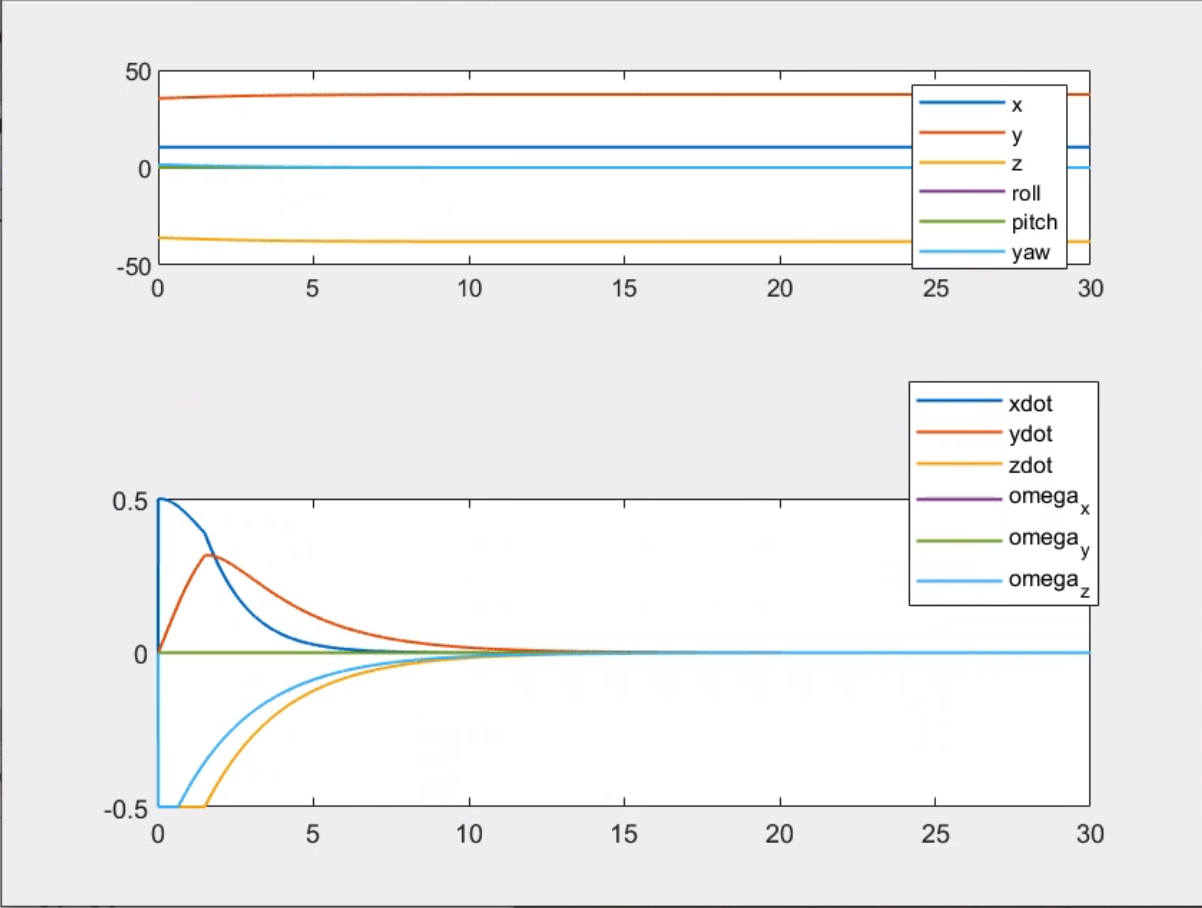
\includegraphics[scale=0.5]{111_ppdot.png}
    \caption{Position and velocity plot for the first task}
    \label{graph_1_1}
\end{figure}

\subsubsection{Q2: What is the behavior if the Horizontal Attitude is enabled or not? Try changing the initial or target orientation in terms of roll and pitch angles. Discuss the behavior.} 
By default the \textit{Horizontal Attitude} is enabled and it has higher priority than the \textit{Vehicle Position} task. 
This results in the UVMS prioritizing the maintaining of a horizontal orientation attitude over the pitch and roll alignment (Figure  \ref{fig:hae}). \\
When the \textit{Horizontal Attitude} is not enabled, the UVMS tries to achieve the alignment between its own frame and the goal one, without taking (of course) into account to maintain the horizontal orientation attitude (Figure  \ref{fig:hane}).

\subsubsection{Q3: Swap the priorities between Horizontal Attitude and the Vehicle Position control task. Discuss the behavior.}
The problem is the same as before. With the priorities swapped, if the target has roll or pitch different from zero, the vehicle will try to achieve such orientation. \\
Therefore, when we change the priorities, the behavior observed during the simulation is almost the same as when we disable the \textit{Horizontal Attitude} task  (Figure  \ref{fig:hane}).\\
Moreover, swapping the priority is wrong because the \textit{Horizontal Attitude} is a safety task, which should have higher priority than an action-defining task. 
\clearpage

%%%%%%% near images %%%%%%% 
\begin{figure}[!htb]
\centering
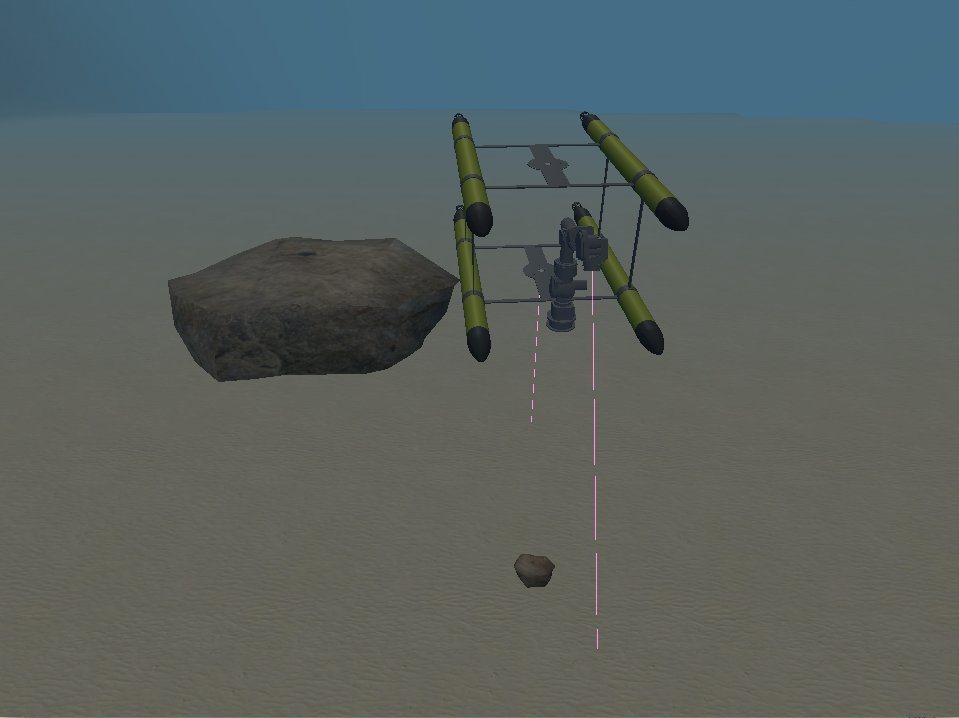
\includegraphics[width=.5\textwidth]{112_HAenabled.png}\caption{\textit{Horizontal Attitude} enabled, the robot is parallel with the seafloor.}
\label{fig:hae}
\vspace{5px}
\centering
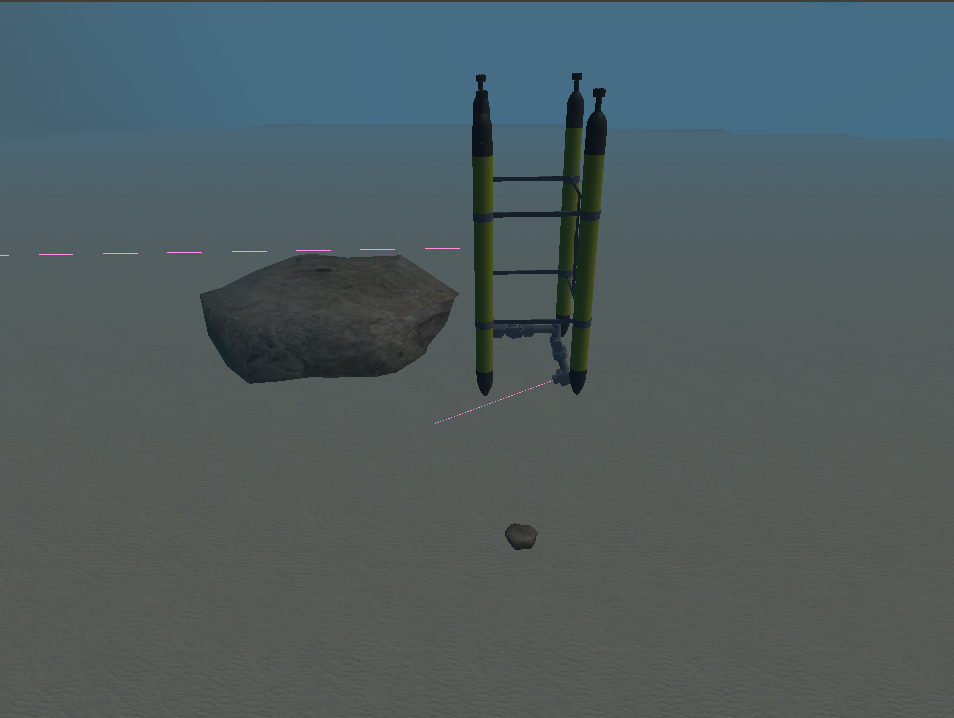
\includegraphics[width=.5\textwidth]{112_HANotenabled.png}\caption{\textit{Horizontal Attitude} not enabled, the robot is not parallel with the seafloor.}
\label{fig:hane}
\end{figure}
%%%%%%% %%%%%%%%%% %%%%%%% 


\subsubsection{Q4: What is the behavior if the Tool Position control task is active and what if it is disabled? Which of the settings should be used for a Safe Waypoint Navigation action?}
If \textit{Tool Position} control task is enabled and it has higher priority than the \textit{Vehicle Position} control task, the UVMS tries to achieve the goal position with the arm. \\
For this reason, we defined two different goal position, the first for the vehicle and the other one for the end-effector. \\
The settings we used for the Safe Waypoint Navigation are:
\begin{itemize}
\item enable \textit{Manipulability} to avoid loss of dexterity,
\item enable \textit{Horizontal Attitude},
\item use the \textit{Vehicle Position} to reach the vehicle desired position,
\item enable the \textit{Tool Position} only when the safe position is reached, to avoid that this task drags the vehicle in a not safe way. 
\end{itemize}
\clearpage

\subsection{Adding a safety minimum altitude control objective}
Initialize the vehicle at the position:
\begin{displaymath}
\begin{bmatrix} 48.5 & 11.5 & -33 & 0 & 0 &-\pi/2\end{bmatrix}^\top
\end{displaymath} 
Choose as target point for the vehicle position the following one:
\begin{displaymath}
\begin{bmatrix} 50 & -12.5 & -33 & 0 & 0 &-\pi/2 \end{bmatrix}^\top
\end{displaymath}

Goal: Implement a task to control the altitude from the seafloor. Check that at all times the minimum distance from the seafloor is guaranteed.

\subsubsection{Q1: Report the hierarchy of task used and their priorities. Comment how you choose the priority level for the minimum altitude.}

\noindent
\vspace{5px}
The new \textbf{hierarchy} of tasks is:
\begin{enumerate}
	\item Minimum Altitude
	\item Manipulability
	\item Horizontal Attitude
	\item Vehicle Position
\end{enumerate}

\noindent
\vspace{5px}
The new task implemented: \\
\textbf{Minimum Altitude} [R, I, S], it is a safety task, so it has high priority. This task improves to the UVMS the ability to avoid collisions with the seafloor.

\subsubsection{Q2: What is the Jacobian relationship for the Minimum Altitude control task? How was the task reference computed?}
We need to control the movement along the $z$ axis, so we use the same Jacobian of the \textit{Vehicle Position}, but selecting only the component related to the $z$ axis.

%%%%%%% Jacobian Matrix %%%%%%% 
\begin{equation}
\large
\boldsymbol{J}_{mav}=\begin{bmatrix} 0 & 0 & 0 & 0 & 0 & 1
\end{bmatrix}
    \begin{bmatrix}
     & \underset{3\times 3}{\boldsymbol{0}} & \underset{ 3\times 3}{^{w}\boldsymbol{R}_{v}} \\
     \underset{ 6\times 7}{\boldsymbol{0}} \\
     & \underset{ 3\times 3}{^{w}\boldsymbol{R}_{v}} & \underset{3\times 3}{\boldsymbol{0}} \\
    \end{bmatrix}
\end{equation}
%%%%%%% %%%%%%% %%%%%%% %%%%%%% 

Again, notice that in order to select the desired component we used the vector [0 0 0 0 0 1] because the control variable uses the convention [Roll Pitch Yaw X Y Z].

\noindent
\vspace{5px}
We compute the \textbf{task reference} as: 
\begin{equation}
\large
    ^{w}\dot{\overline{\boldsymbol{x}}}_{mav} = k((d_{limit}+\Delta)- {^w}d_{sensor})) %delta
\end{equation}
where:
\begin{itemize}
    \item $k$ is the control gain.
    \item $d_{limit}$ is the desired minimum distance from the seafloor.
    \item $ \Delta $ is the safety distance at which the activation of the task starts to trigger.
    \item $^w d_{sensor}$ is the third component  of the distance vector, measured by the sensor and projected on the world frame.
\end{itemize} 

\begin{figure}[t]
    \centering
    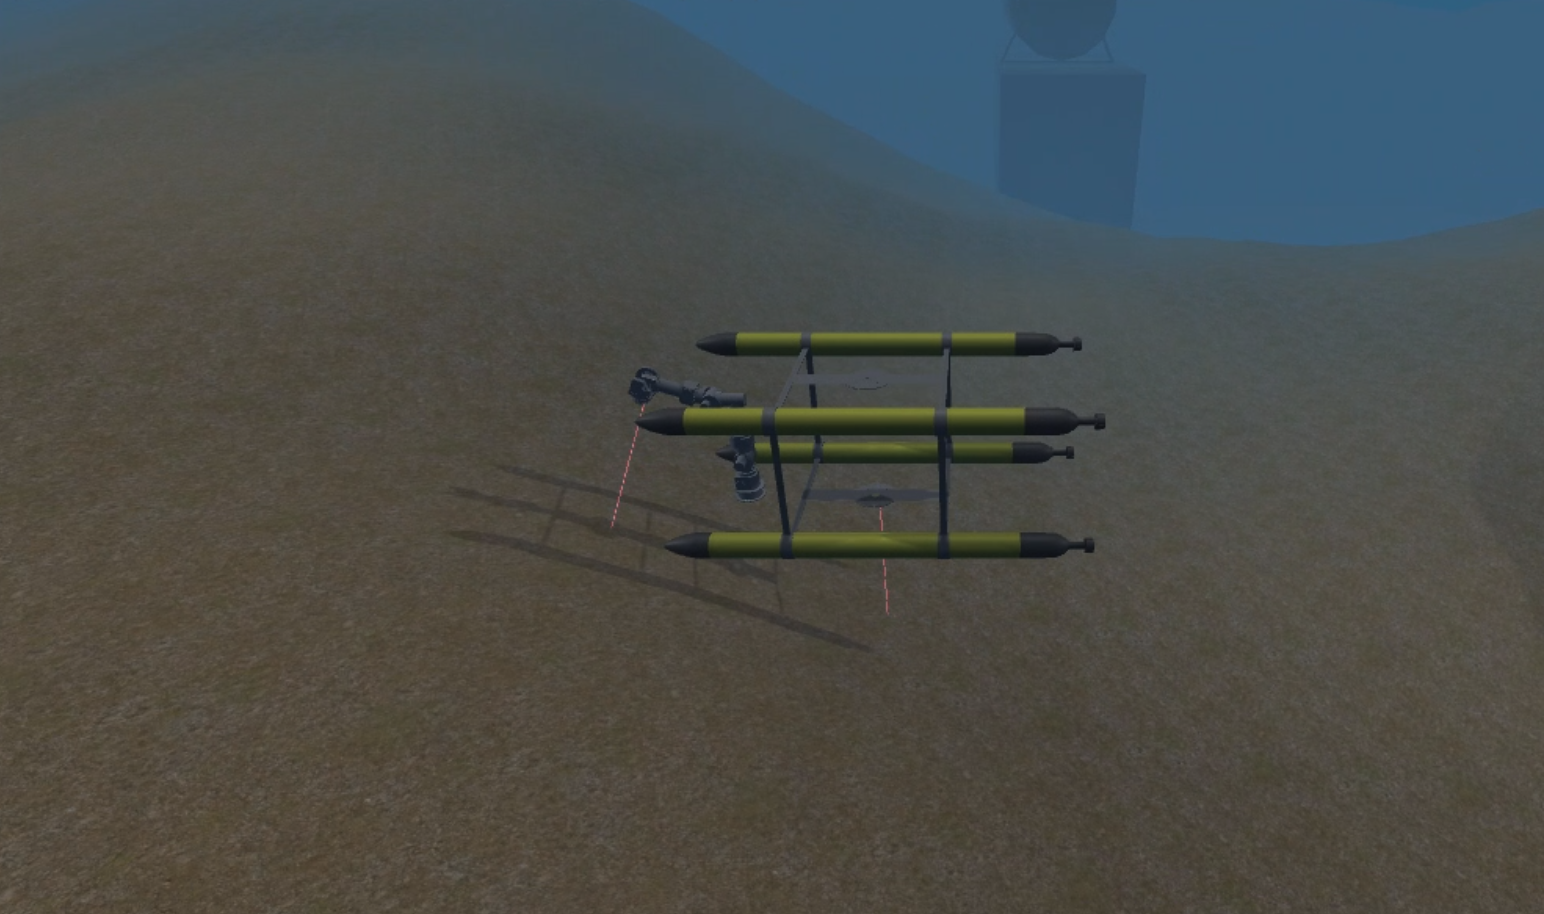
\includegraphics[scale=0.4]{122_MAV1m.png}
    \caption{Minimum altitude is enabled and the robot is following the seafloor}
    \label{images_2_1}
\end{figure}

%%Gray box for defining code implemented or referred to
%\colorbox{mygray}{\parbox{0.9\textwidth}{Code for Exercise: \\
%\texttt{Compute Task Reference -> MAV Control}\\
%}}

\subsubsection{Q3: Try imposing a minimum altitude of 1, 5, 10 m respectively. What is the behavior?}
In order to test this task we ran the simulation with different values for the minimum altitude, all with the same $k$ gain (equal to $0.2$).

\begin{itemize}
    \item \textbf{10 m:} The UVMS has initial position below this threshold, so it starts floating towards the surface very quickly (it is possible also to notice this huge vertical velocity $\dot{z}$, in the graph (Figure \ref{10m_ppdot})). 
    Of course, the task is not accomplished because the target position is far from the threshold, therefore, this value does not seem a reasonable one. % 
    \item \textbf{5 m:} Again, the task is triggered immediately, because the initial position is below the minimum altitude value. This control task is a safety one, so every time the UVMS is under the minimum altitude, the activation is enabled and it has the highest priority. 
    Again, it seems not a reasonable value. (Figure \ref{5m_ppdot}).
    \item \textbf{1 m:} The control task is no more active at the starting instant. The UVMS starts to accomplish the \textit{Vehicle Position} task and, when the seafloor presents an hill, the vehicle starts to follow its shape (Figure \ref{1m_ppdot}). 
\end{itemize}
However, there could be some troubles during the navigation if the seafloor has a steep slope: the front of the vehicle could collide with the soil, because the sensor is placed in the center of the vehicle.


\subsubsection{Q4: How was the sensor distance processed?}
 
 Since we are interested only in the component along the $z$ axis, the $^{v}\boldsymbol{d}_{sensor}$ vector is build as:
 
 \begin{equation}
 \large
 \begin{bmatrix}0 & 0 & d_{seafloor} \end{bmatrix}^\top
 \end{equation}
 
 \skip 0.5cm
 
 However, ${^{v}\boldsymbol{d}_{sensor}}$ is the distance vector measured by the sensor, projected on the vehicle frame. Since we need to project it on the world frame, we apply the following rotation matrix:
 
 \begin{equation}
 \large
     {^{w}\boldsymbol{d}_{sensor}} = {^{w}\boldsymbol{R}_{v}} {^{v}\boldsymbol{d}_{sensor}}
 \end{equation}


% %Gray box for defining code implemented or referred to
%\colorbox{mygray}{\parbox{0.9\textwidth}{Code for Exercise: \\
%\texttt{TO DO}\\
%\texttt{TO DO}
%}}

%%%%%%%% MINI PAGE IMAGES 10 m %%%%%%%%
\begin{figure}[htpb] 
\begin{minipage}{0.40\textwidth}  
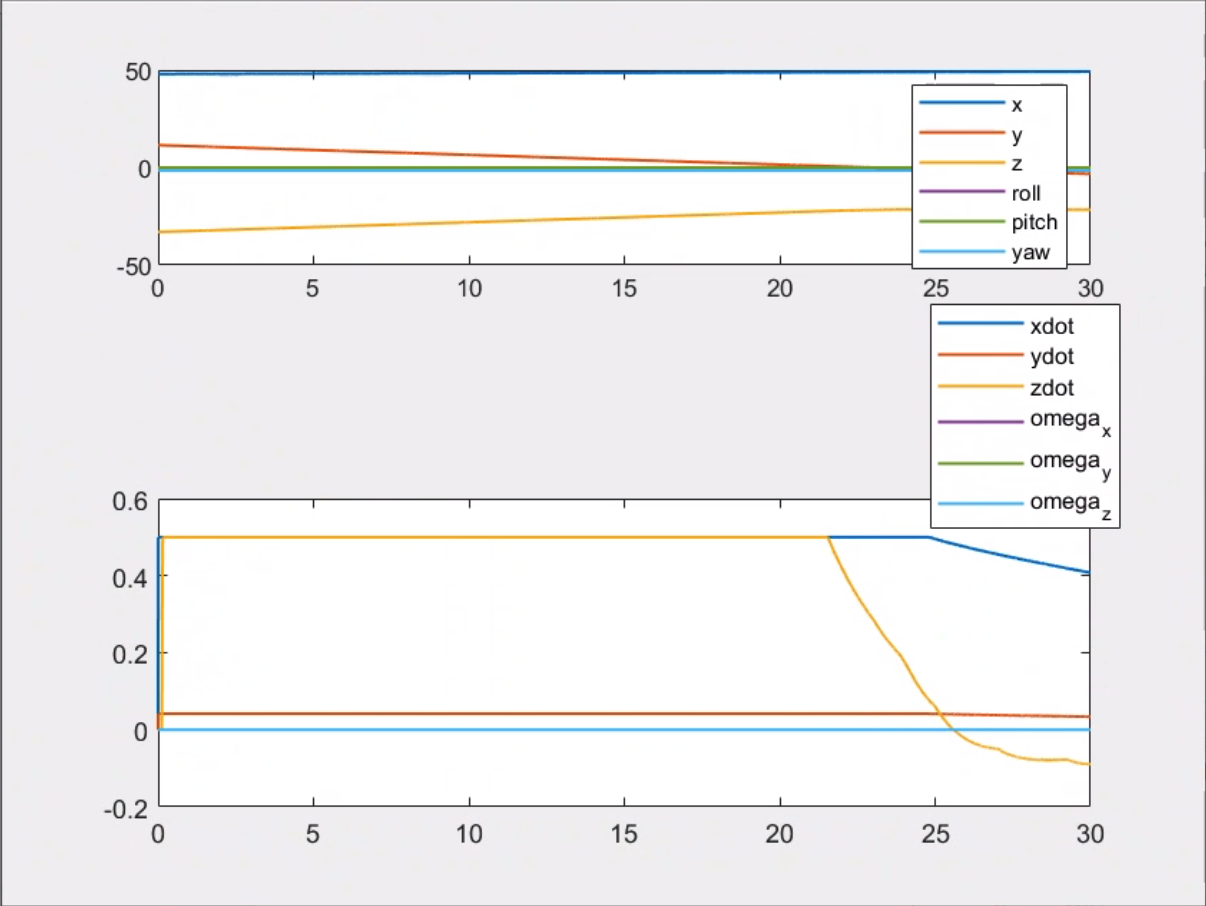
\includegraphics[width=\textwidth]{123_10m_ppdot.png}
\caption{Position and velocity plot with Minimum Altitude threshold of 10m}\label{10m_ppdot} 
\end{minipage}  
\hspace{0.2\textwidth} 
\begin{minipage}{0.43\textwidth}  
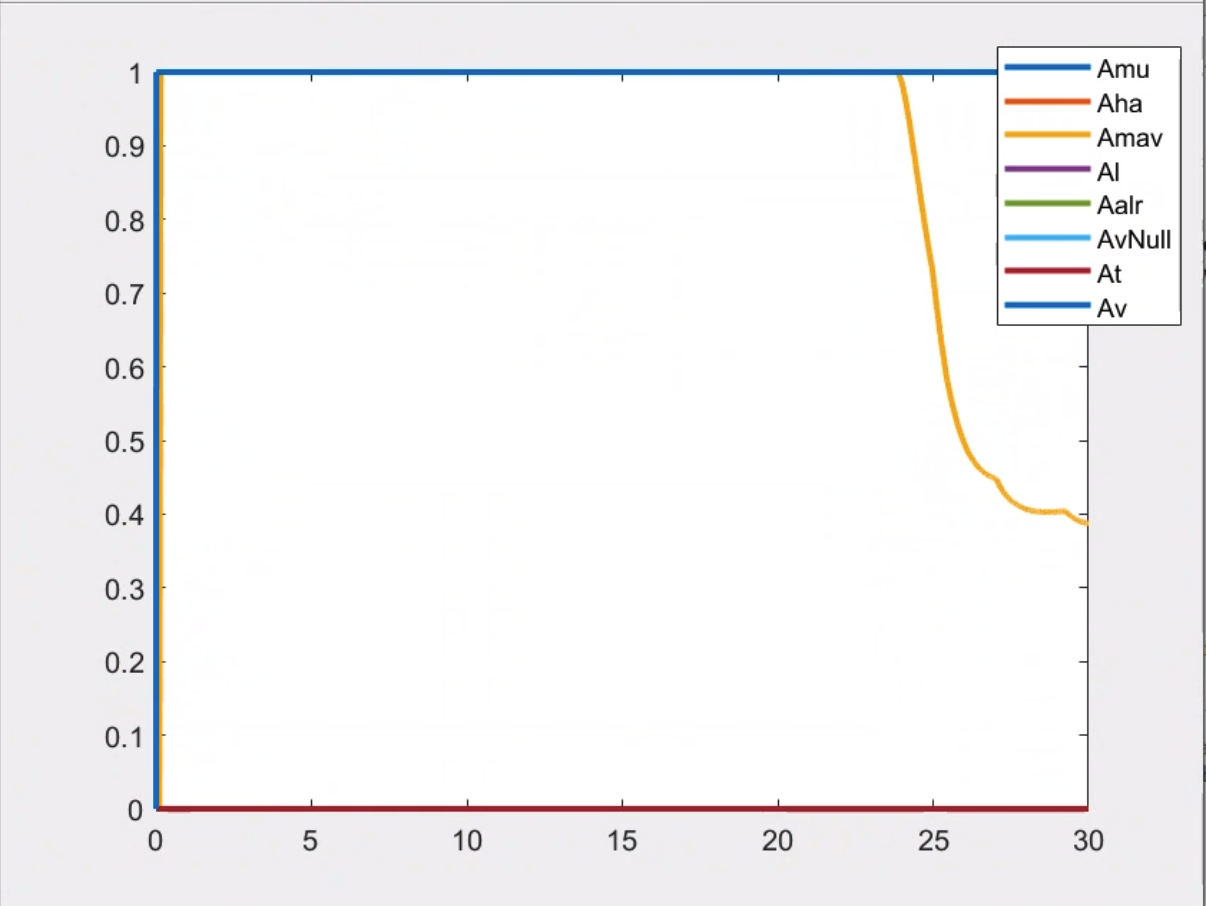
\includegraphics[width=\textwidth]{123_10m_A.png}
\caption{Activation plot (threshold 10m) }\label{10m_A} 
\end{minipage} 
\end{figure}
%%%%%%%% MINI PAGE IMAGES %%%%%%%%

%%%%%%%% MINI PAGE IMAGES 5 m %%%%%%%%
\begin{figure}[htpb] 
\begin{minipage}{0.40\textwidth}  
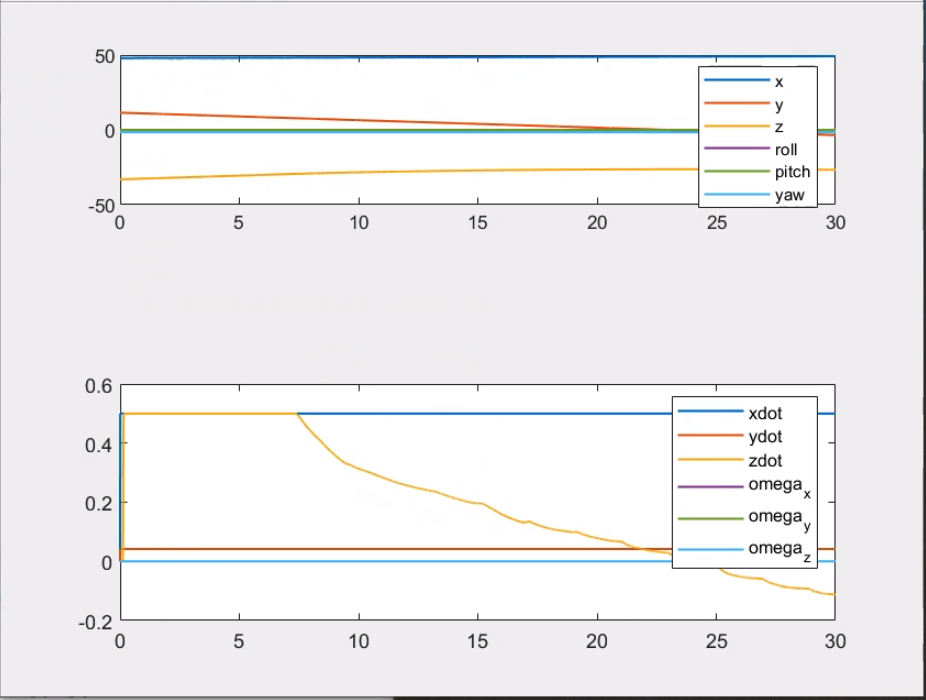
\includegraphics[width=\textwidth]{123_5m_ppdot.png}
\caption{Position and velocity plot with Minimum Altitude threshold of 5m}\label{5m_ppdot} 
\end{minipage}  
\hspace{0.2\textwidth} 
\begin{minipage}{0.43\textwidth}  
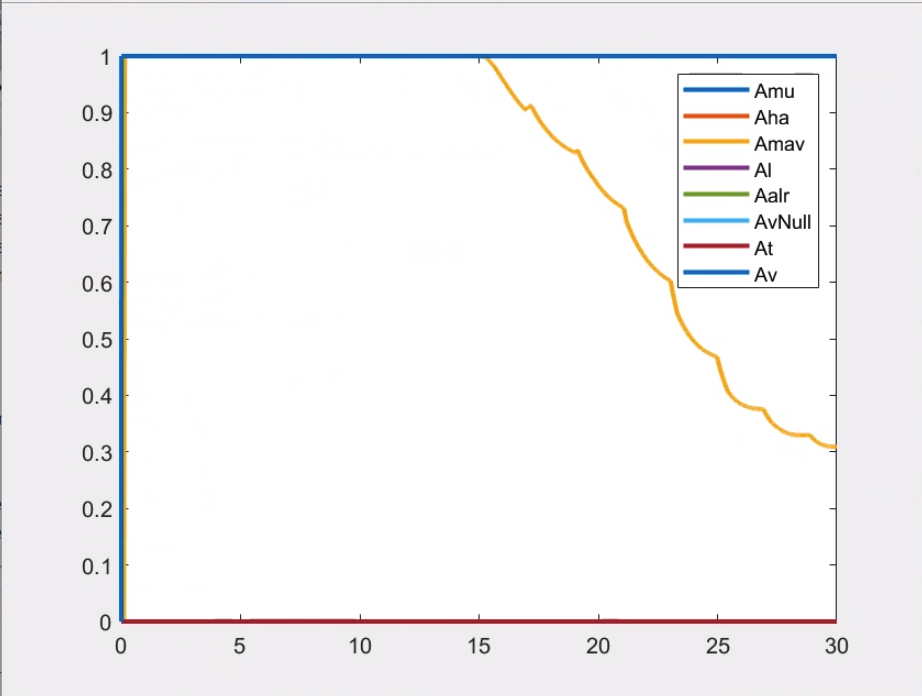
\includegraphics[width=\textwidth]{123_5m_A.png}
\caption{Activation plot (threshold 5m) }\label{5m_A} 
\end{minipage} 
\end{figure}
%%%%%%%% MINI PAGE IMAGES %%%%%%%%

%%%%%%%% MINI PAGE IMAGES 1 m %%%%%%%%
\begin{figure}[htpb] 
\begin{minipage}{0.40\textwidth}  
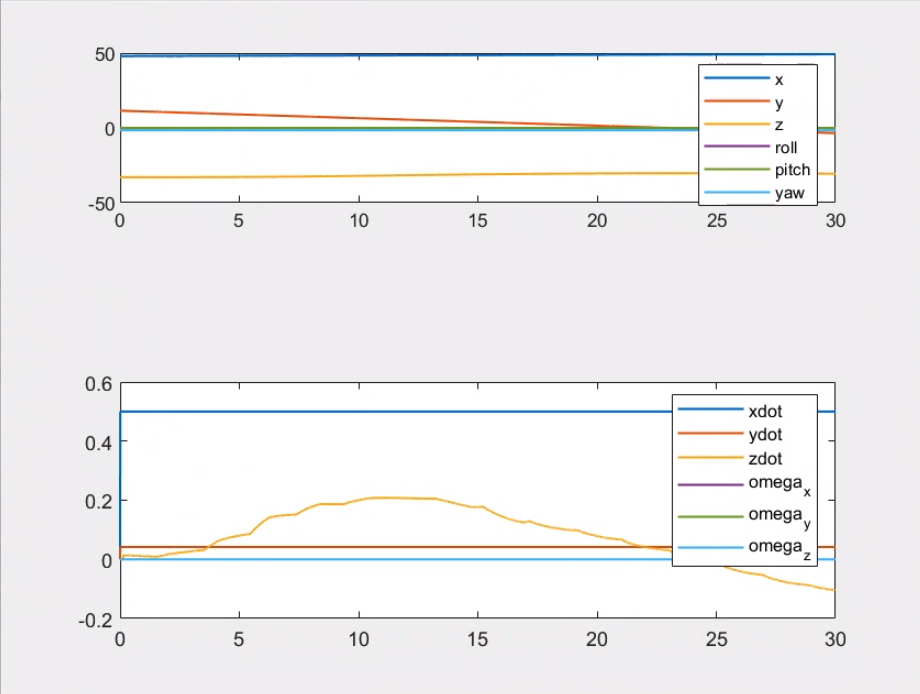
\includegraphics[width=\textwidth]{123_1m_ppdot.png}
\caption{Position and velocity plot with Minimum Altitude threshold of 1m}\label{1m_ppdot} 
\end{minipage}  
\hspace{0.2\textwidth} 
\begin{minipage}{0.43\textwidth}  
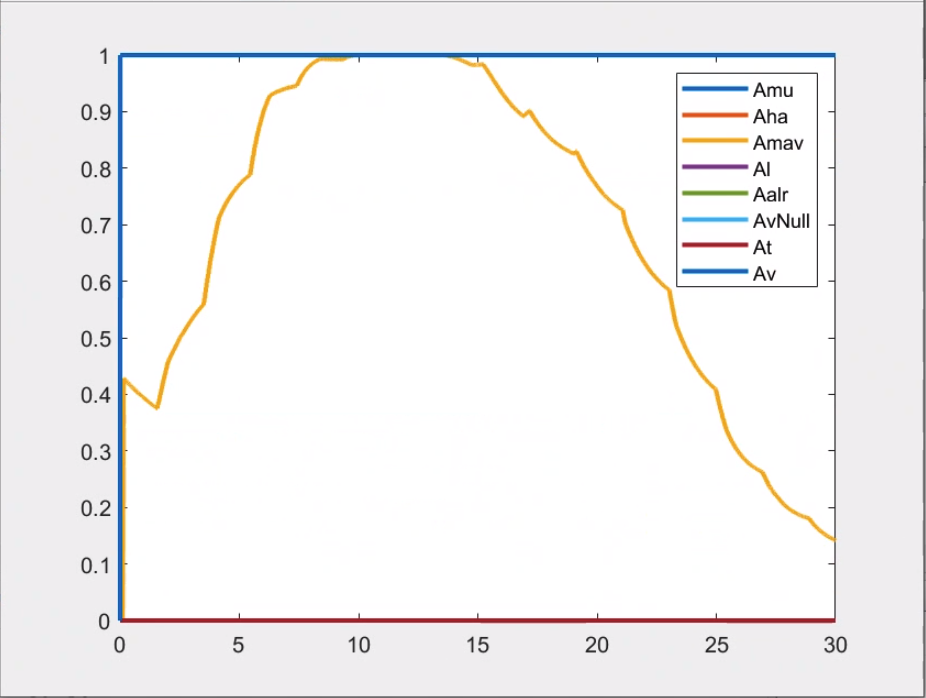
\includegraphics[width=\textwidth]{123_1m_A.png}
\caption{Activation plot (threshold 1m) }\label{1m_A} 
\end{minipage} 
\end{figure}
%%%%%%%% MINI PAGE IMAGES %%%%%%%%

\clearpage

\section{Exercise 2: Implement a Basic “Landing” Action.}
\subsection{Adding an altitude control objective}
Initialize the vehicle at the position:
\begin{displaymath}
\begin{bmatrix} 10.5 & 37.5 & -38 & 0 & -0.06 & 0.5 \end{bmatrix}^\top
\end{displaymath} 

Goal: add a control task to regulate the altitude to zero.

\subsubsection{Q1: Report the hierarchy of task used and their priorities. Comment how you choose the priority level for the altitude control task.}

\noindent
\vspace{5px}
The new \textbf{hierarchy} of tasks is:
\begin{enumerate}
	\item Manipulability
	\item Horizontal attitude
	\item Landing
\end{enumerate}

\noindent
\vspace{2px}
\begin{description}
\item \textbf{Landing} [R, E, AD], it is the new task. It is an Action Defining task, so it has the same level of priority of the \textit{Vehicle Position}.
\end{description}

\noindent
The task \textit{Minimum Altitude} is not enabled now, because we are required to land , therefore the UVMS needs to go below the fixed minimum altitude threshold.

\begin{figure}[h]
    \centering
    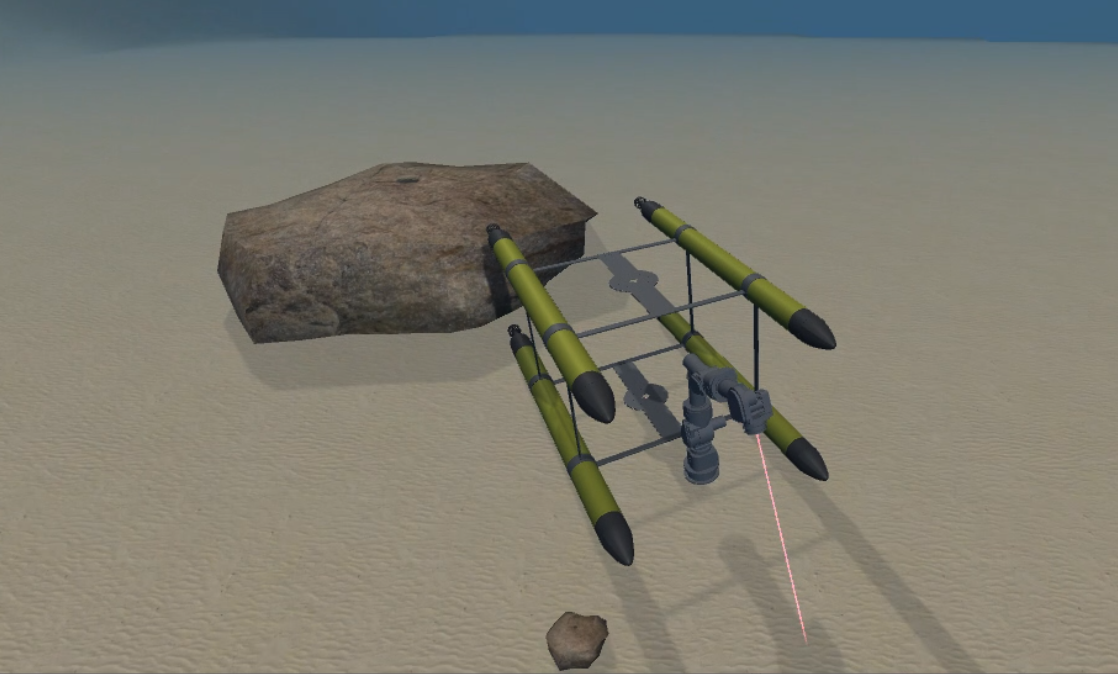
\includegraphics[scale=0.4]{211_Landing.png}
    \caption{Implemented basic \textit{Landing} action}
    \label{images_2_3_1}
\end{figure}

\subsubsection{Q2: What is the Jacobian relationship for the Altitude control task? How was the task reference computed?}

\noindent
\vspace{5px}
The Jacobian relationship for the \textit{Landing} is:
\begin{equation}
\large
\boldsymbol{J}_{land}=\begin{bmatrix} 0 & 0 & 0 & 0 & 0 & 1
\end{bmatrix}
    \begin{bmatrix}
     & \underset{3\times 3}{\boldsymbol{0}} & \underset{ 3\times 3}{^{w}\boldsymbol{R}_{v}} \\
     \underset{6\times 7}{\boldsymbol{0}} \\
     & \underset{ 3\times 3}{^{w}\boldsymbol{R}_{v}} & \underset{3\times 3}{\boldsymbol{0}} \\
    \end{bmatrix}
\end{equation}
As before, the Jacobian is required to control only the component along the $z$ axis.
 
\noindent
\vspace{5px}
We compute the \textbf{task reference} as:

\begin{equation}
\large
    ^{w}\dot{\overline{\boldsymbol{x}}}_{land} = k((d_{landing} + \Delta_{safeguard}) - ^w d_{sensor}) %delta
\end{equation}
where:
\begin{itemize}
    \item $k$ is the control gain.
    \item $d_{landing}$ is the distance from the seafloor, in this case is obviously $0$.
    \item $\Delta_{safeguard}$ is set to $0.15m$  to avoid interpenetration between UVMS and the seafloor.
    \item $^w d_{sensor}$ is the component along the $z$ axis of the distance vector measured by the sensor and projected on the world frame.
\end{itemize} 

%%Gray box for defining code implemented or referred to
%\colorbox{mygray}{\parbox{0.9\textwidth}{Code for Exercise: \\
%\texttt{TO DO}\\
%\texttt{TO DO}
%}}

\subsubsection{Q3: how does this task differs from a minimum altitude control task?}
There are two major difference:
\begin{itemize} 
\item The first one is that \textit{Landing} is not a safety task, but an action-defining one. While the \textit{Minimum Altitude} task is used to avoid collisions with the seafloor, the \textit{Landing} task defines an action (as the \textit{Vehicle Position} task), therefore it has lower priority.\\
\item The second difference is that \textit{Minimum Altitude} is an inequality task rather than \textit{Landing} which is an equality one. As visible on the plots below (Figure \ref{213}), MAV is active when we are under the defined threshold while \textit{Landing} is triggered only when a prerequisite is satisfied and it is not deactivated until we land on the seafloor.
\end{itemize}
%%%%%%%% MINI PAGE IMAGES %%%%%%%%
\begin{figure}[!h]
    \centering
    \begin{minipage}{0.50\textwidth}
    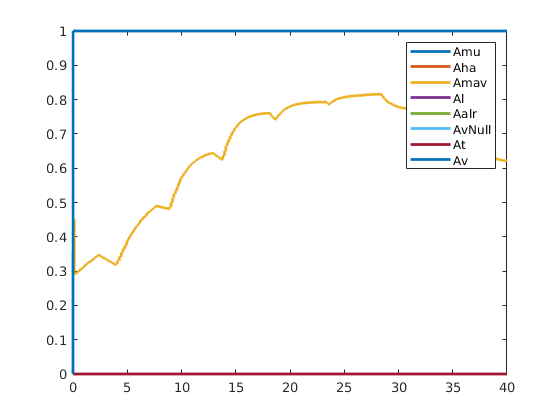
\includegraphics[scale=0.5]{213_MAV_A.png}
    \caption{Graph MAV}
    \label{213}
    \end{minipage}
\hfill
    \centering
    \begin{minipage}{0.50\textwidth}
    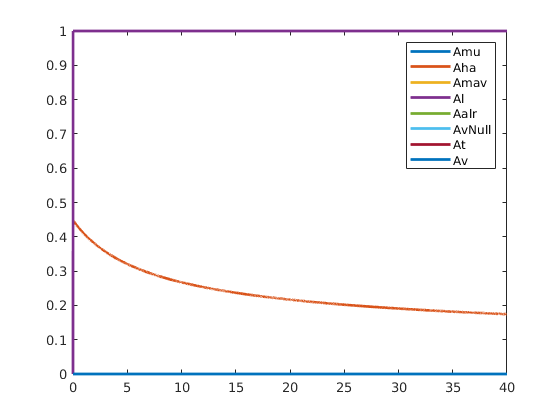
\includegraphics[scale=0.5]{213_Landing_A.png}
    \caption{Graph Landing}
    \end{minipage}
\end{figure}
%%%%%%%% MINI PAGE IMAGES %%%%%%%%

\clearpage

\subsection{Adding mission phases and change of action}
Initialize the vehicle at the position:
\begin{displaymath}
\begin{bmatrix} 8.5 & 38.5 & -36 & 0 & -0.06 & 0.5 \end{bmatrix}^\top
\end{displaymath} 
Use a "safe waypoint navigation action" to reach the following position: 
\begin{displaymath}
\begin{bmatrix} 10.5 & 37.5 & -38 & 0 & -0.06 & 0.5 \end{bmatrix}^\top
\end{displaymath} 
When the position has been reached, land on the seafloor using the basic "landing" action.

\subsubsection{Q1: Report the unified hierarchy of tasks used and their priorities.}

We have two different actions, with this \textbf{hierarchy} and the following activations: 
%%%%%% TABLE %%%%%%%%%
\begin{center}
\begin{tabular}{ | c | c | c | c |}
\hline
 Control Task & \texttt{Code name} & Action A & Action B \\
\hline
 Minimum Altitude Vehicle &  \texttt{mav} & Active & Inactive  \\  
 Manipulabity &  \texttt{mu} & Active & Active  \\
 Horizontal Attitude &  \texttt{ha} & Active & Active \\
 Landing & \texttt{l} &Inactive & Active \\
 Vehicle Position &  \texttt{v} &Active & Inactive \\
 \hline
\end{tabular}
\end{center}

\begin{description}
\item Action A: the UVMS performs the safe waypoint navigation. All the safety tasks are enabled. 
\item Action B: the UVMS simply lands on the seafloor, performing the previous exercise task. Of course, the \textit{Minimum Altitude} task is deactivated .
\end{description}
 
%%%%%% TABLE %%%%%%%%%


%%Gray box for defining code implemented or referred to
%\colorbox{mygray}
%{\parbox{0.9\textwidth}{Code for Exercise: \\
%\texttt{ComputeMissionPhase}\\
%}}

\subsubsection{Q2: How did you implement the transition from one action to the other?}

The transition between Action A and Action B is triggered by the achievement of the vehicle target position. We compute the cartesian error between the goal frame and the vehicle frame and, when the error is below the given threshold (in this case $0.1m$), the mission phase changes. 

When we want to deactivate a running task, we use a Decreasing Bell Shape function in order to perform a smooth transition. In this case, the \textit{Minimum Altitude} and \textit{Vehicle Position} tasks are both deactivated at the start of the second phase. In a similar way, when we want to activate a task, we use an Increasing Bell Shape function to perform a smooth transition, as we do for the \textit{Landing} task. 
We compute the slope of such functions based on the mission phase time: this help us to fix the time interval (in our case, $0.2$ seconds) in which the vehicle switches from an Action to the other and let us achieve a smooth shape, avoiding discontinuities in the actuation of the motors.
\begin{figure}[!htb]
    \centering
    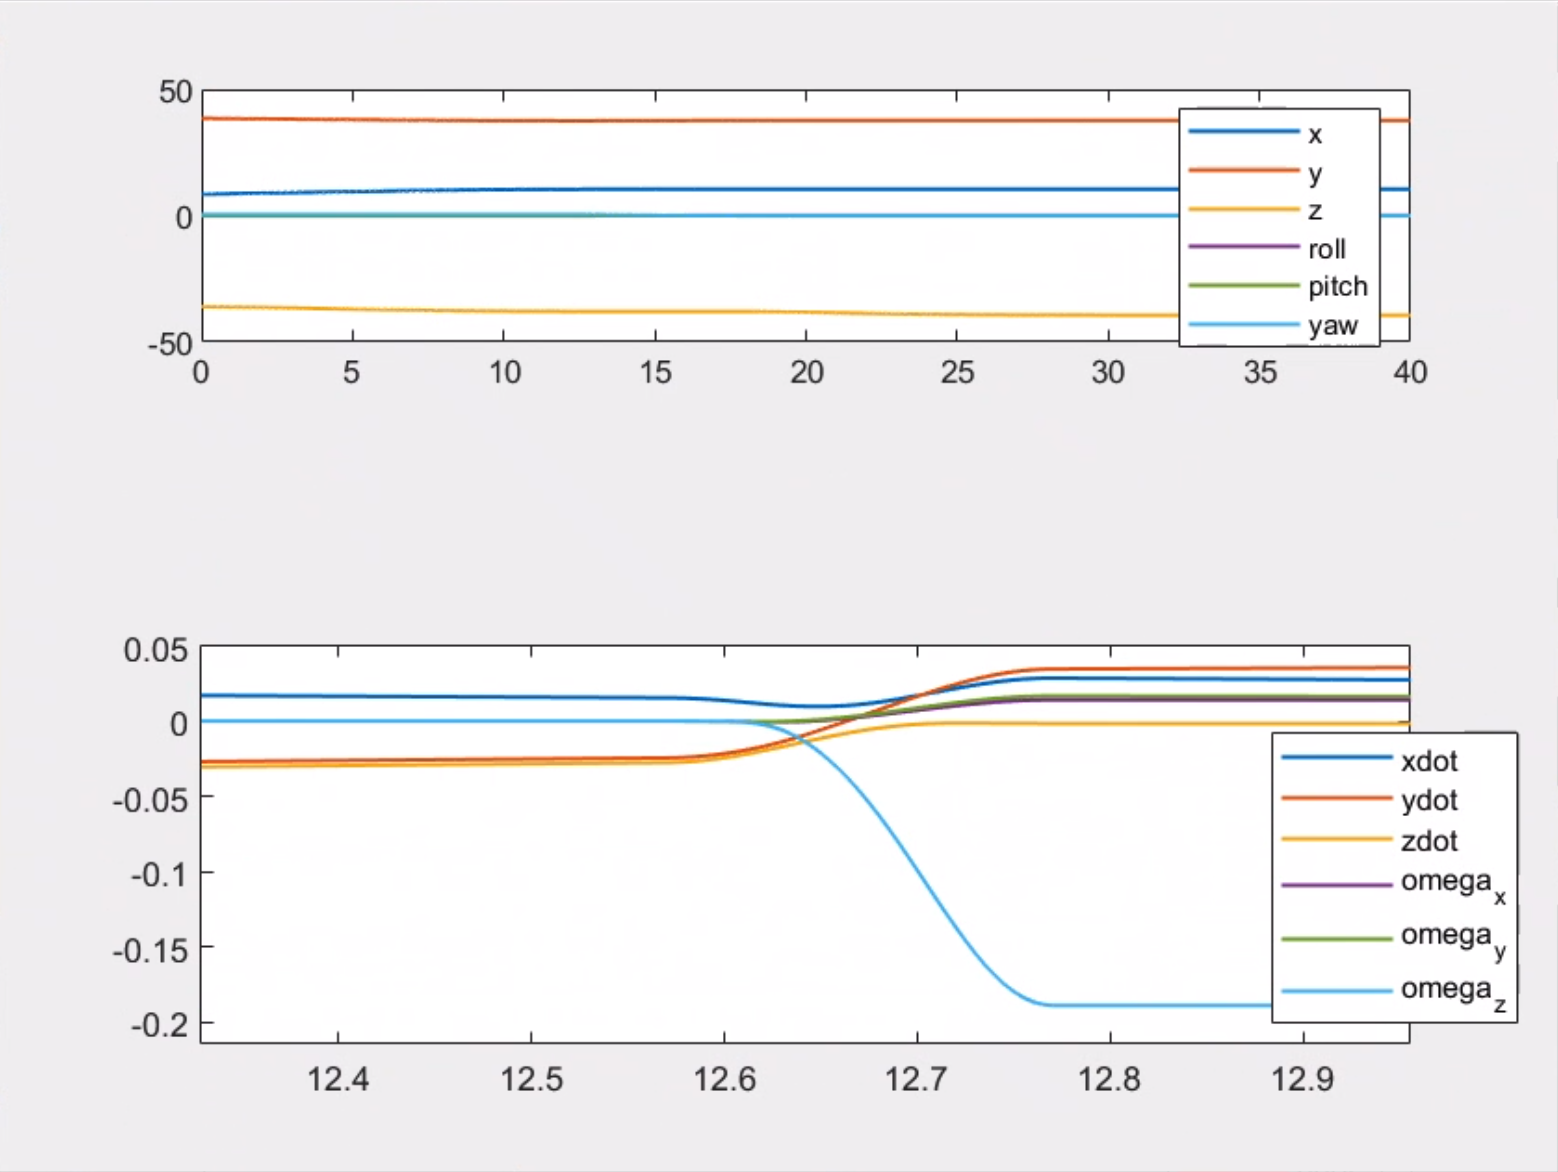
\includegraphics[scale=0.25]{222_smooth_ppdot.png}
    \caption{Zoom of the smooth change}
    \label{images_2_3_1}
\end{figure}

We found this more adeguate than the previous attempt, in which we performed the shape based on the error distance.
\clearpage

\section{Exercise 3: Improve the “Landing” Action}
\subsection{Adding an alignment to target control objective}
If we use the landing action, there is no guarantee that we land in from of the nodule/rock. We need to add additional constraints to make the vehicle face the nodule. The position of the rock is contained in the variable \texttt{rock\_center}. 

Initialize the vehicle at the position:
\begin{displaymath}
\begin{bmatrix} 8.5 & 38.5 & -36 & 0 & -0.06 & 0.5 \end{bmatrix}^\top
\end{displaymath} 
Use a "safe waypoint navigation action" to reach the following position: 
\begin{displaymath}
\begin{bmatrix} 10.5 & 37.5 & -38 & 0 & -0.06 & 0.5 \end{bmatrix}^\top
\end{displaymath} 
Then land, aligning to the nodule.

Goal: Add an alignment task between the longitudinal axis of the vehicle ($x$ axis) and the nodule target. In particular, the $x$ axis of the vehicle should align to the projection, on the inertial horizontal plane, of the unit vector joining the vehicle frame to the nodule frame.

\subsubsection{Q1: Report the unified hierarchy of tasks used and their priorities. Comment the behavior.}
We have three different actions, with this hierarchy and activations:
%%%%%% TABLE %%%%%%%%%
\begin{center}
\begin{tabular}{ | c | c | c | c | c |}
\hline
 Control Task & \texttt{Code name} & Action A & Action B & Action C\\
 \hline
 Minimum Altitude Vehicle &  \texttt{mav} & Active & Active & Inactive\\  
 Manipulabity &  \texttt{mu} & Active & Active & Active\\
 Horizontal Attitude &  \texttt{ha} & Active & Active & Active\\
 Alignment to the Rock & \texttt{alr} & Inactive & Active & Active \\
 Landing & \texttt{l} &Inactive & Inactive & Active \\
 Vehicle Position &  \texttt{v} &Active & Inactive & Inactive\\
 \hline
\end{tabular}
\end{center}
%%%%%% TABLE %%%%%%%%%
\vspace{5px}
\noindent
The new task is:
\begin{description}
\item \textbf{Alignment to the Rock} [R, I, P], it is a prerequisite task, so it has higher priority than the action-defining tasks. Inequality, because we admit a $\Delta$ of errors equal to $0.07$.   \ocio 
\end{description}

\begin{figure}[h]
    \centering
    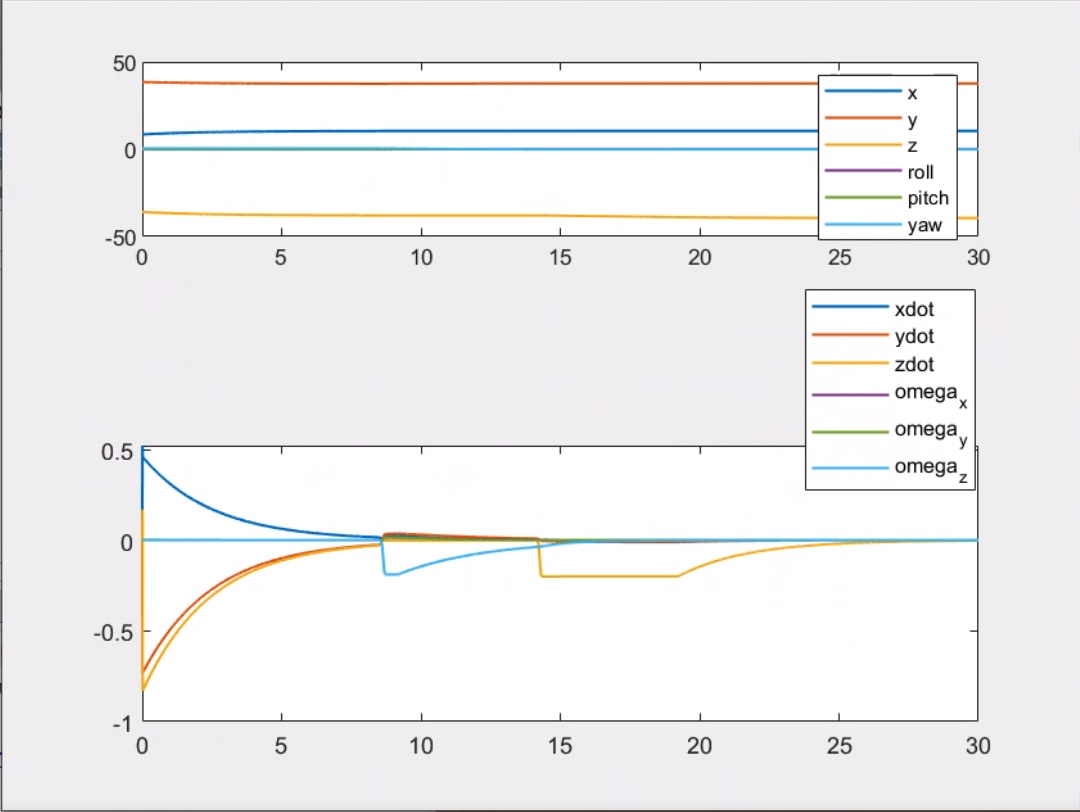
\includegraphics[scale=0.3]{311_ppdot.png}
    \caption{Positions and velocities during the three actions.}
    \label{graphes3}
\end{figure}

\begin{description}
	\item Action A, again, a safe waypoint navigation with all the safety tasks enabled (Figure \ref{311a}). 
	\item Action B, it is the action that performs the alignment to the rock, with all the safety task enabled (Figure \ref{311b}). 
	\item Action C, \textit{Alignment to the Rock} is not disable because, while the UVMS starts landing, we disable smoothly the alignment. In this case, while the robot is performing the landing, it continue to rotate to optimize the orientation (Figure \ref{311c}).
\end{description}



%%%%%%% near images %%%%%%% 
\begin{figure}[htp]
\centering
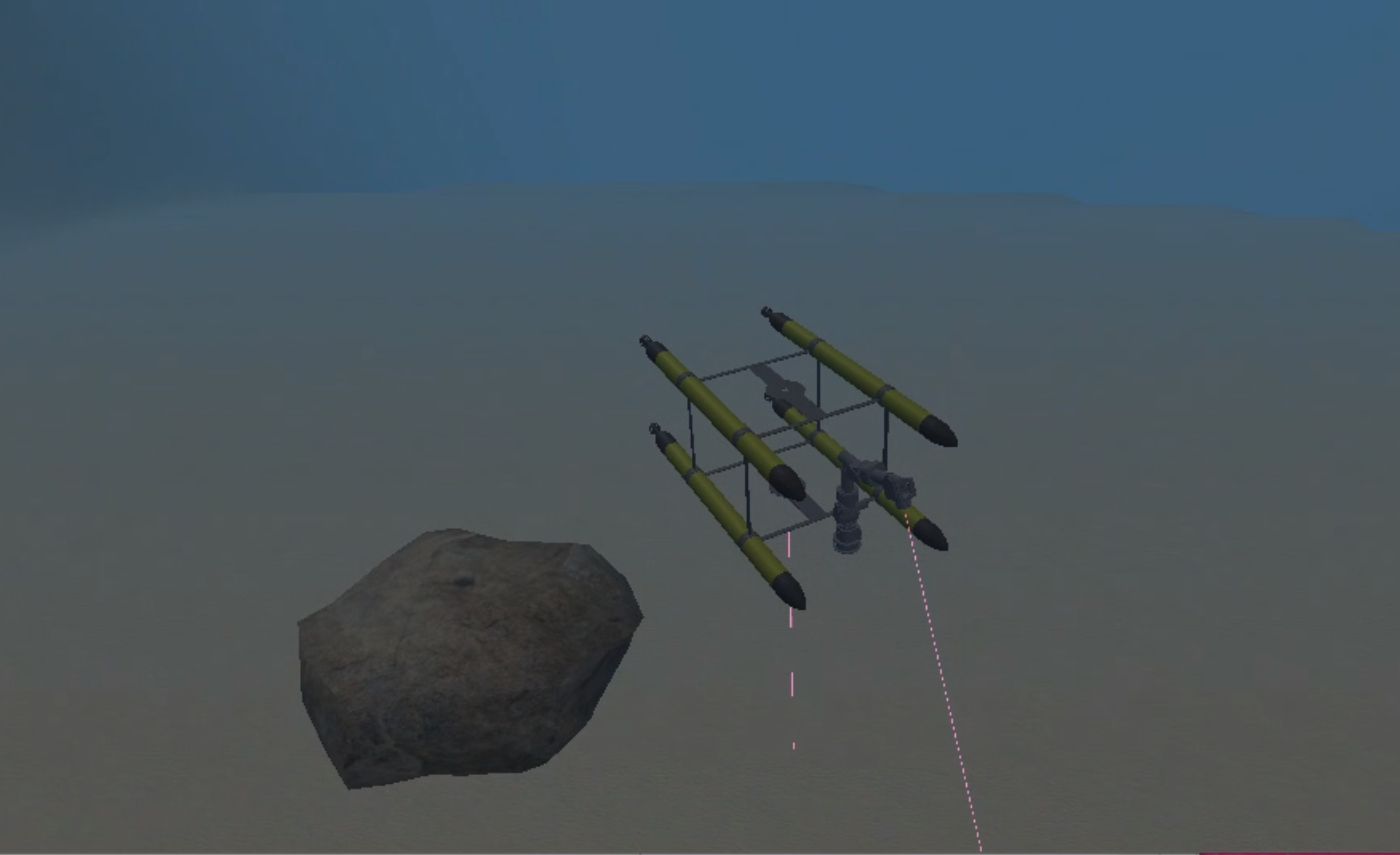
\includegraphics[width=.6\textwidth]{312_Nav.png}\caption{Action A: Navigation till the target position}\label{311a}
\vspace{5px}
\centering
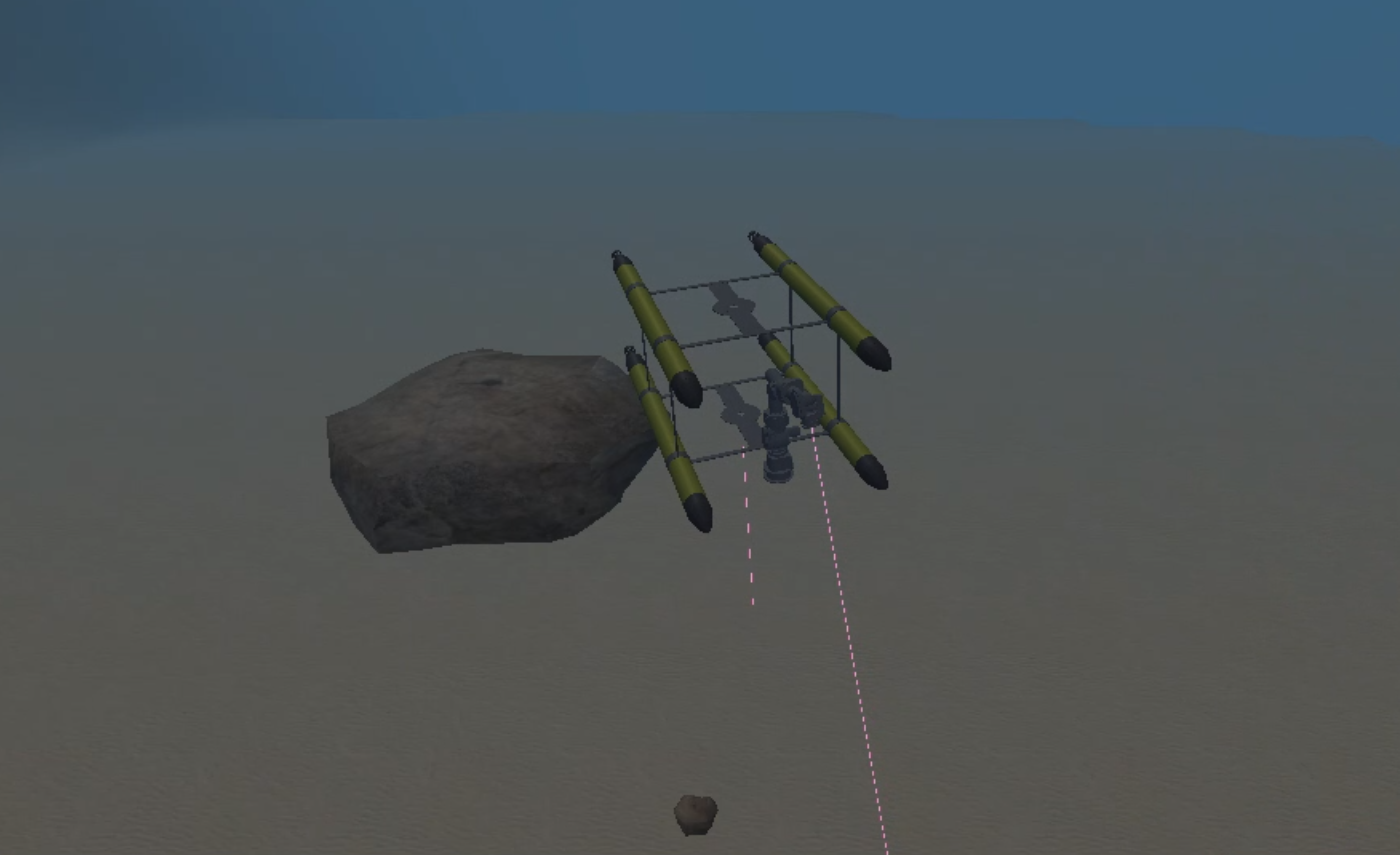
\includegraphics[width=0.6\textwidth]{312_Alr.png}\caption{Action B: Alignment with the rock center}\label{311b}
\vspace{5px}
\centering
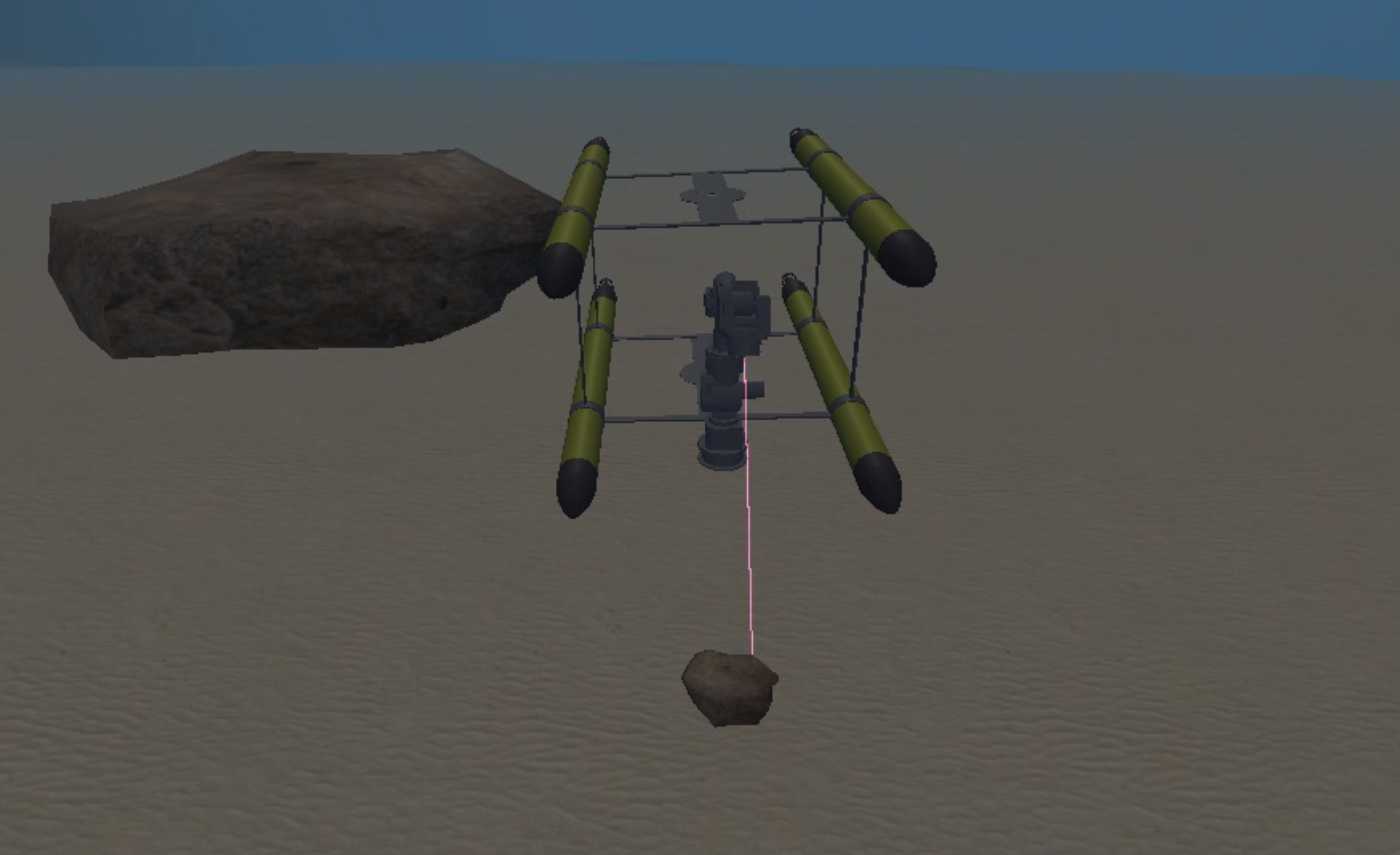
\includegraphics[width=.6\textwidth]{312_Land.png}\caption{Action C: Landing, final action}\label{311c}
\label{fig:missionphase3}
\vspace{5px}
\end{figure}
%%%%%%% %%%%%%%%%% %%%%%%% 
\clearpage

\subsubsection{Q2: What is the Jacobian relationship for the Alignment to Target control task? How was the task reference computed?} \

The Jacobian relationshio for the Alignment starts from here:

\begin{equation}
\large
D_{w}(\boldsymbol \rho)=\boldsymbol J_{alr} \boldsymbol \dot{q}
\end{equation}

Where defining $\boldsymbol J_{alr} $ is our goal.

We know that:
\begin{equation}
\large
D_{w}(\boldsymbol \rho)={^w}\boldsymbol n_{\rho} \dot\theta+\underbrace{\theta D_{w} {^w}{\boldsymbol n_{\rho}}}_{orthogonal}
\end{equation}

We are not interested on the orthogonal components so we can ignore them.

Regarding the first part of the equation,
\begin{equation}
\large
\dot{\theta}={^w}\boldsymbol{\omega}_{v} - {^w}{\boldsymbol\omega_{{rock}}}
\end{equation}

\begin{equation}
\large
D_w(\boldsymbol \rho)={^w}\boldsymbol n_\rho\left({^w}{\boldsymbol \omega}_{v}-{^w}{\boldsymbol \omega_{rock}}\right)
\end{equation}

We need to describe ${^w}{\boldsymbol{\omega}}_{v} \text{ and } \boldsymbol{\omega}_{rock} \text{ in term of } \boldsymbol{\dot{q}} $

\begin{equation}
\large
{^w}\boldsymbol \omega_{v} = 
\underbrace{
    \begin{bmatrix}
     \underset{3\times 3}{\boldsymbol{0}} & \underset{ 3\times 3}{^{w}\boldsymbol{R}_{v}}\\
    \end{bmatrix}
}_{\boldsymbol J_{vehicle}}
\dot{\boldsymbol{q}}
\end{equation}

\begin{equation}
\large
{^w}{\boldsymbol v}_{v}={^w}\boldsymbol \omega_{rock} \wedge {^w} \boldsymbol d
\end{equation}

\begin{equation}
\large
{^w}\boldsymbol w_{rock}=\frac{1}{\left\|{^w} \boldsymbol d^{2}\right\|}\left[{^w}{\boldsymbol d} \wedge\right] {{^w}{\boldsymbol v_{v}}}
\end{equation}

\noindent
We are interested only on the $x$ and $y$ component of ${^w}{\boldsymbol v_{v}}$, to do this we premultiply, like this:

\begin{equation}
\large
{^w}\boldsymbol w_{rock}=\frac{1}{\left\|{^w} \boldsymbol d^{2}\right\|}\left[{^w}{\boldsymbol d} \wedge\right]\left[\begin{array}{lll}
1 & 0 & 0 \\
0 & 1 & 0 \\
0 & 0 & 0
\end{array}\right] {^w}{\boldsymbol v_{v}}
\end{equation}

\begin{equation}
\large
{^w}\boldsymbol v_{v} = 
    \begin{bmatrix}
     \underset{3\times 3}{\boldsymbol{0}} & \underset{ 3\times 3}{^{w}\boldsymbol{R}_{v}} & \underset{3\times 3}{\boldsymbol{0}} \\
    \end{bmatrix}  
\end{equation}

\begin{equation}
\large
{^w}\boldsymbol w_{rock}=
\underbrace{
\frac{1}{\left\|{^w} \boldsymbol d^{2}\right\|}\left[{^w}{\boldsymbol d} \wedge\right]\left[\begin{array}{lll}
1 & 0 & 0 \\
0 & 1 & 0 \\
0 & 0 & 0
\end{array}\right]
    \begin{bmatrix}
     \underset{3\times 3}{\boldsymbol{0}} & \underset{ 3\times 3}{^{w}\boldsymbol{R}_{v}} & \underset{3\times 3}{\boldsymbol{0}} \\
    \end{bmatrix}
}_{\boldsymbol J_{rock}}
    \dot{\boldsymbol{q}}
\end{equation}


\begin{equation}
\large
\boldsymbol J_{\text {alr }}={^w}{\boldsymbol n_{\rho}}[{ \boldsymbol J_{vehicle} - \boldsymbol J_{rock}}]
\end{equation}

\subsubsection{Q3: Try changing the gain of the alignment task. Try at least three different values, where one is very small. What is the observed behaviour?} 
We performed tests with different gain values for the task reference:
\begin{itemize}
	\item Very Small = $0.1$
	\item Medium = $0.6$
	\item Big = $1.2$
\end{itemize}
First, looking at positions and velocities graphs, it is clear that between the medium (Figure \ref{ppdot_w_m}) and the big gain (Figure \ref{ppdot_w_b}) there are no such important differences, with the big gain that transition between the two phases are not so smooth as for the medium one. Of course, the saturation helps the case with the big gain to not perform a too high velocity. 
For the very small gain, the resulted graph is very different (Figure \ref{ppdot_w_s}), becausethe very low velocity performed during the alignment doesn't help to reach the desired position. In our 30 seconds simulation is impossible for the UVMS to align correctly. However, also improving the simulation time, it is normal that it is too slow to accomplish our goal.

From the point of view of the activations and the errors, there are not different results than before. Medium and big gain graphs are very similar (almost identical) and the very small gain graph confirm the previous sentences.
%%%%%%%% MINI PAGE IMAGES %%%%%%%%
\begin{figure}[htpb] 
\begin{minipage}{0.40\textwidth}  
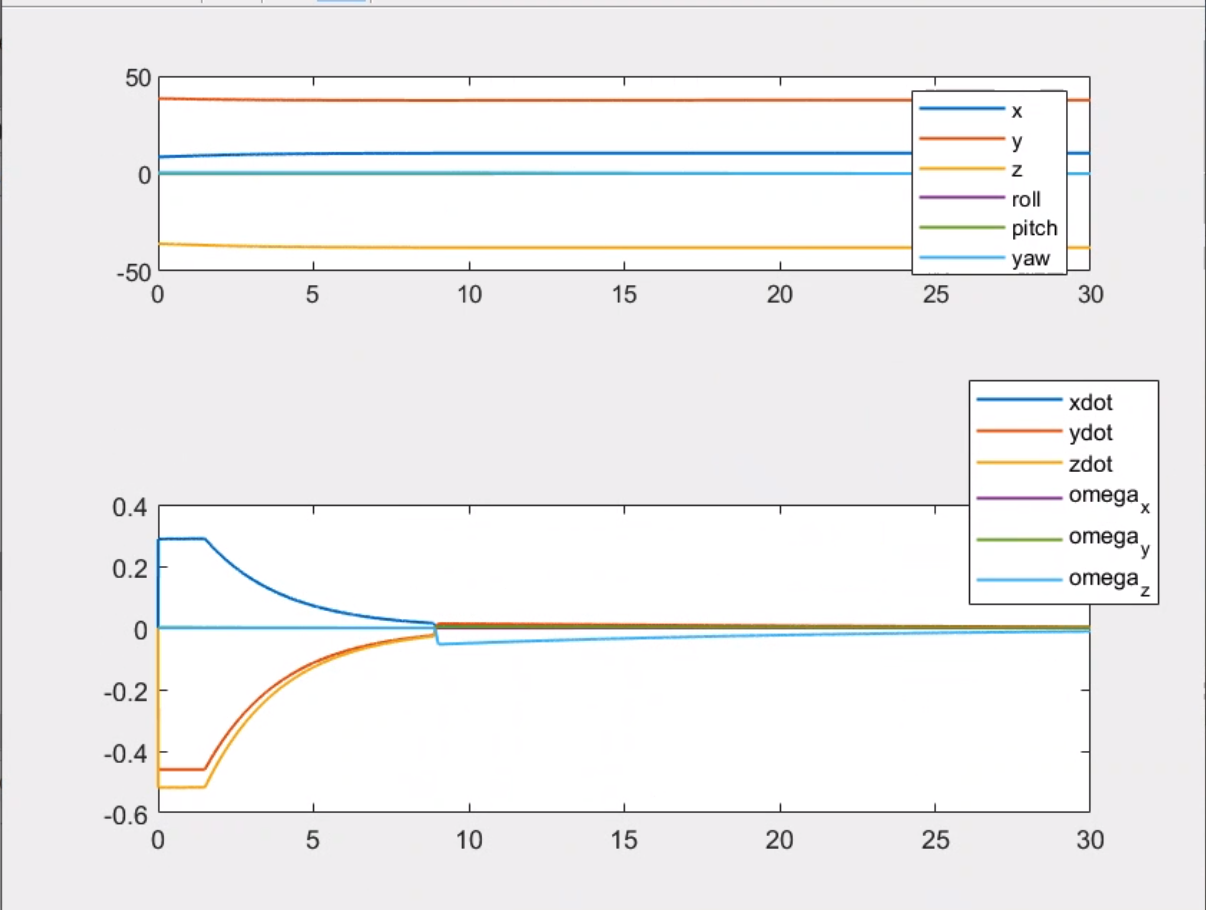
\includegraphics[width=\textwidth]{313_s_ppdot.png}
\caption{Positions and Velocity with small gain}\label{ppdot_w_s} 
\end{minipage}  
\hspace{0.2\textwidth} 
\begin{minipage}{0.40\textwidth}  
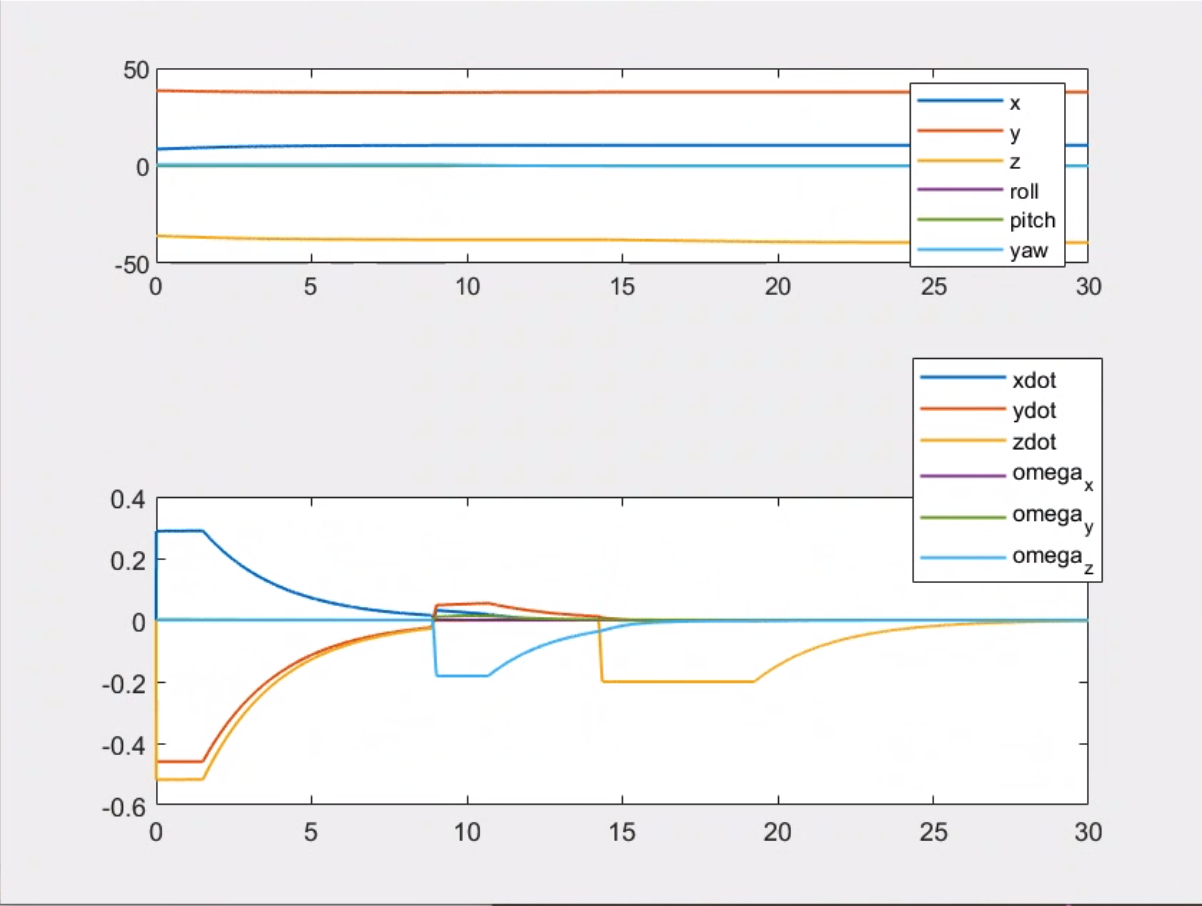
\includegraphics[width=\textwidth]{313_m_ppdot.png}
\caption{Positions and Velocity with medium gain}\label{ppdot_w_m} 
\end{minipage} 
\hspace{0.2\textwidth} 
\begin{minipage}{0.40\textwidth}  
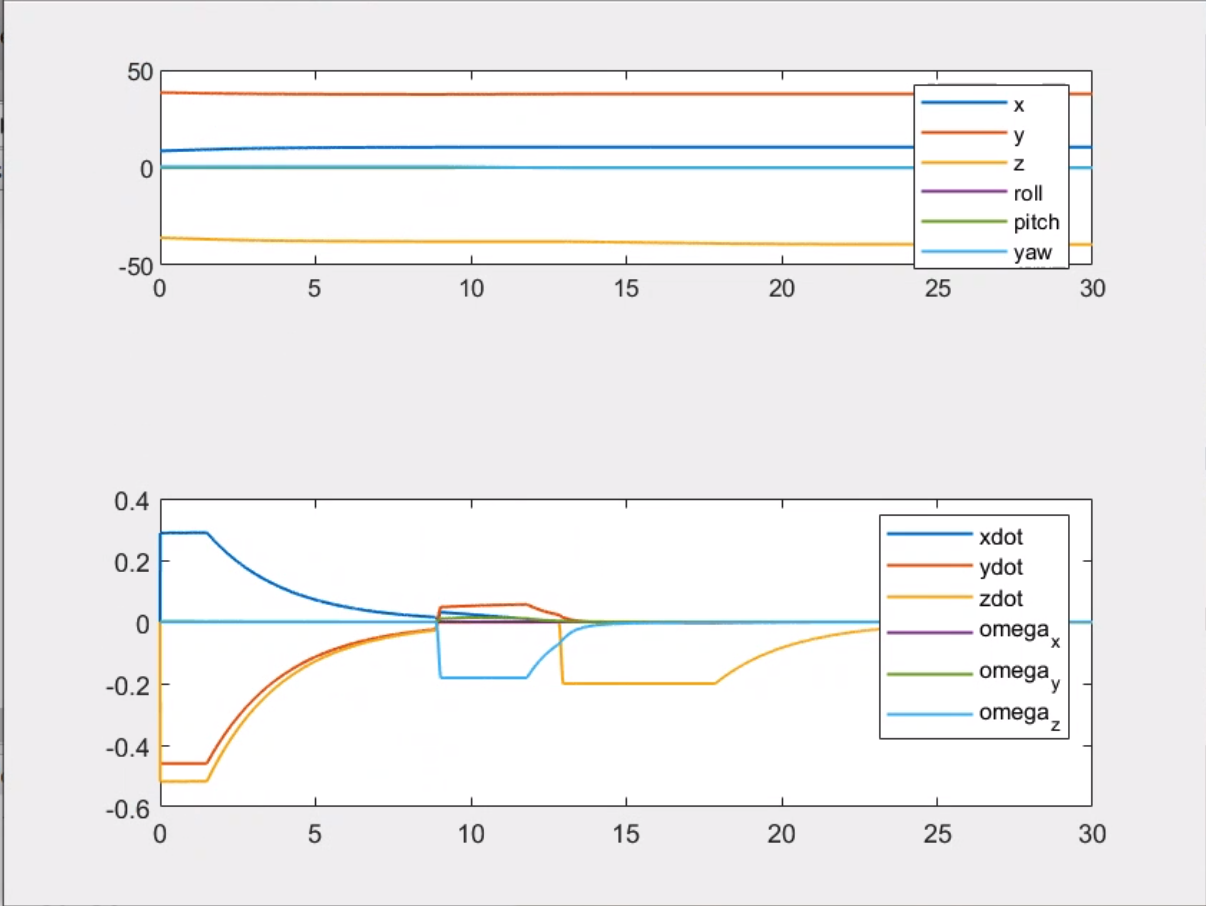
\includegraphics[width=\textwidth]{313_b_ppdot.png}
\caption{Positions and Velocity with big gain}\label{ppdot_w_b} 
\end{minipage}
\end{figure}
%%%%%%%% MINI PAGE IMAGES %%%%%%%%
\begin{figure}[htpb] 
\begin{minipage}{0.40\textwidth}  
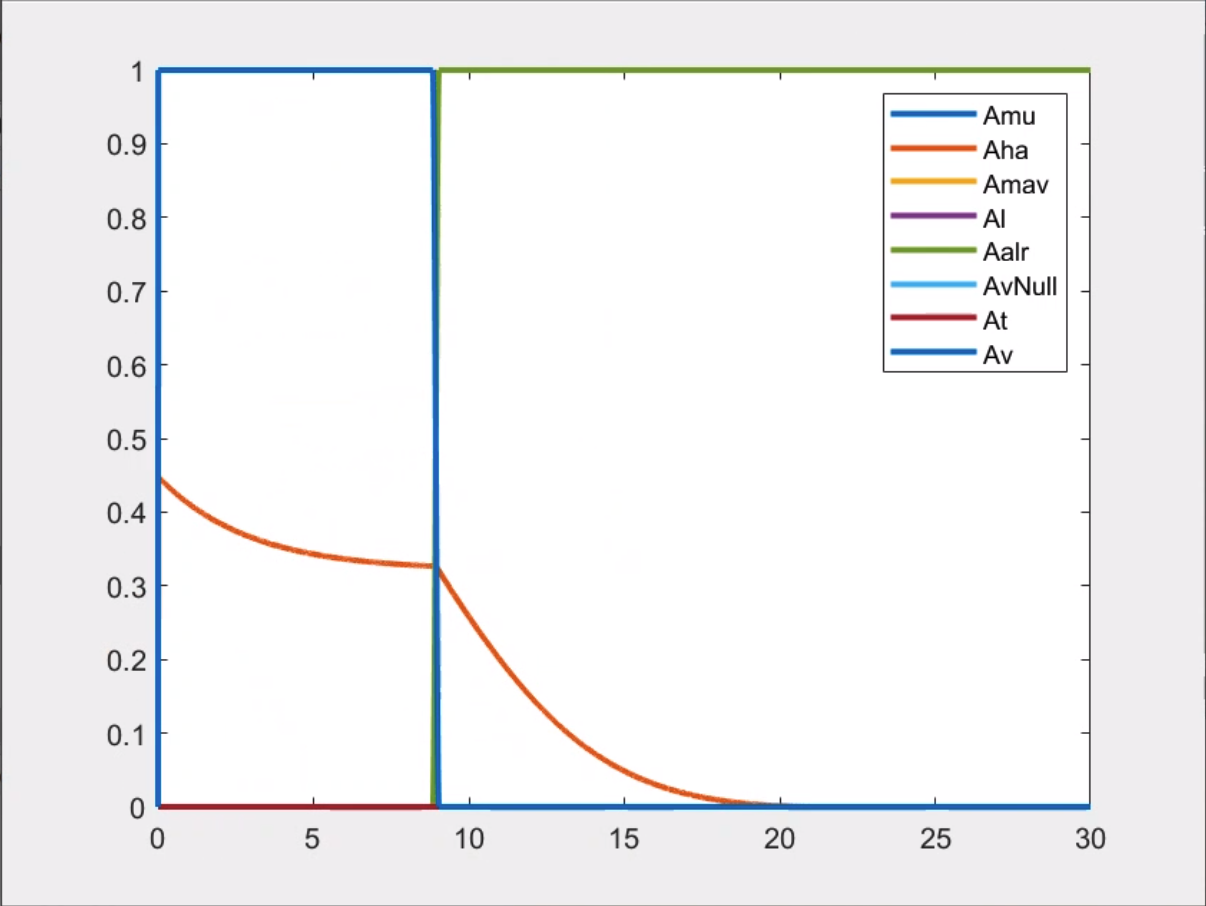
\includegraphics[width=\textwidth]{313_s_Activation.png}
\caption{Activations with very small gain}\label{act_w_s} 
\end{minipage}  
\hspace{0.2\textwidth} 
\begin{minipage}{0.40\textwidth}  
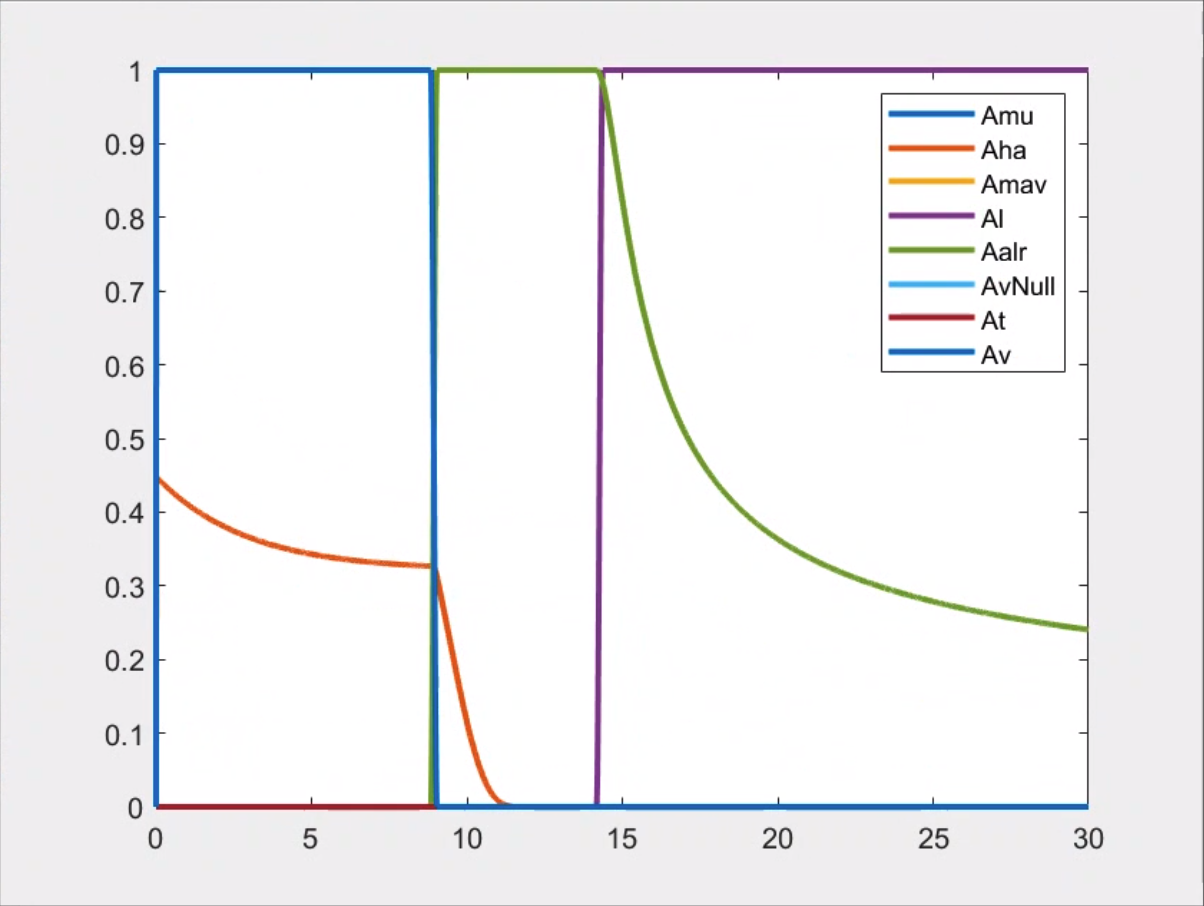
\includegraphics[width=\textwidth]{313_m_Activation.png}
\caption{Activations with medium gain}\label{act_w_m} 
\end{minipage} 
\hspace{0.2\textwidth} 
\begin{minipage}{0.40\textwidth}  
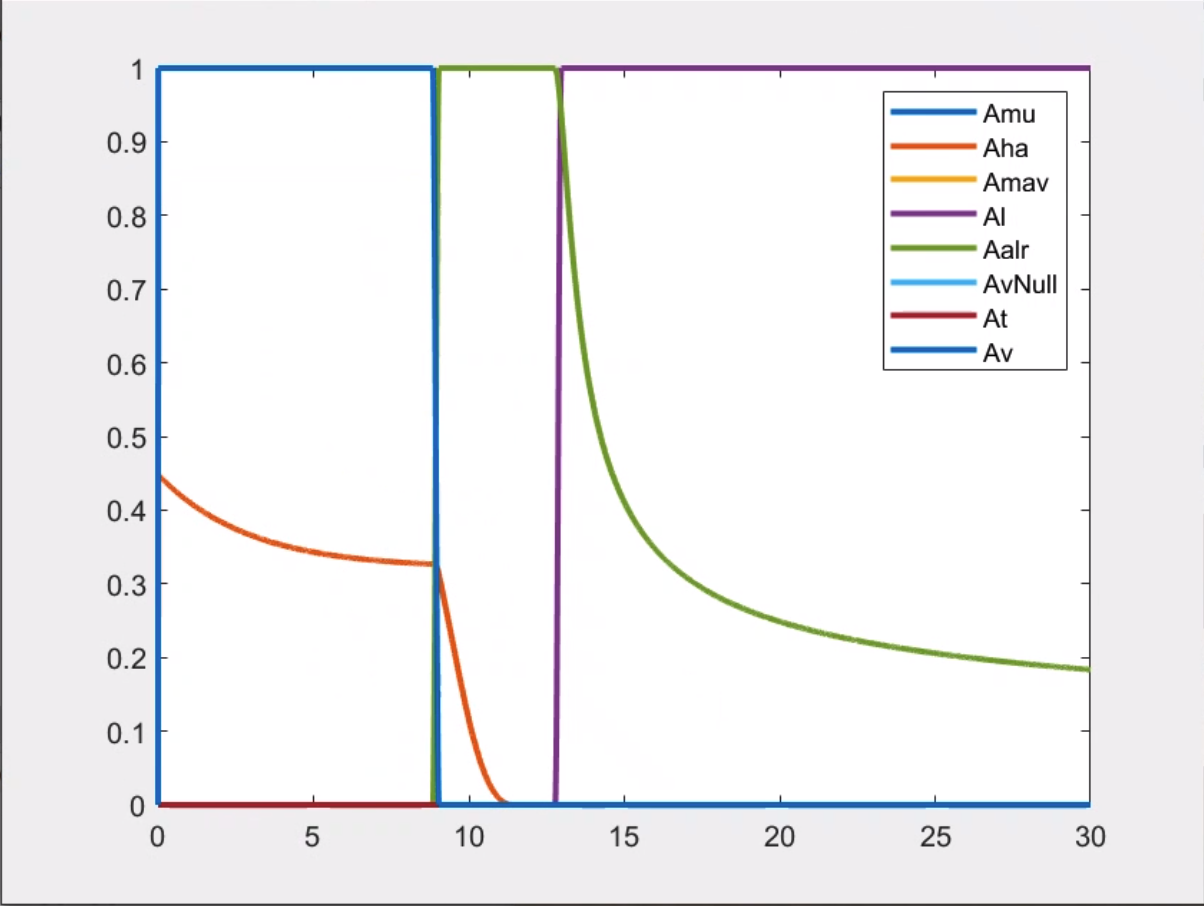
\includegraphics[width=\textwidth]{313_b_Activation.png}
\caption{Activations with big gain}\label{act_w_b} 
\end{minipage}
\end{figure}
%%%%%%%% MINI PAGE IMAGES %%%%%%%%
\begin{figure}[htpb] 
\begin{minipage}{0.40\textwidth}  
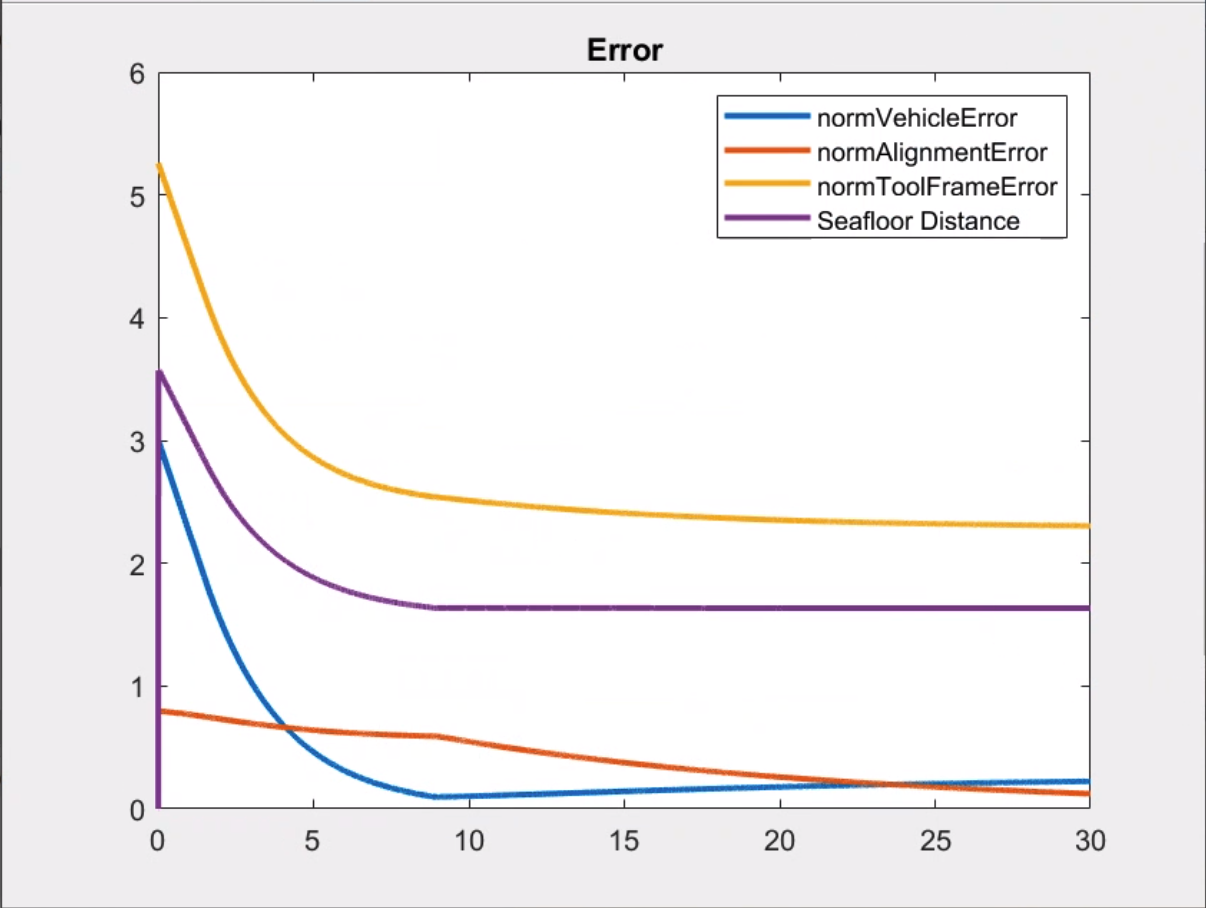
\includegraphics[width=\textwidth]{313_s_Errors.png}
\caption{Errors with small}\label{err_w_s} 
\end{minipage}  
\hspace{0.2\textwidth} 
\begin{minipage}{0.40\textwidth}  
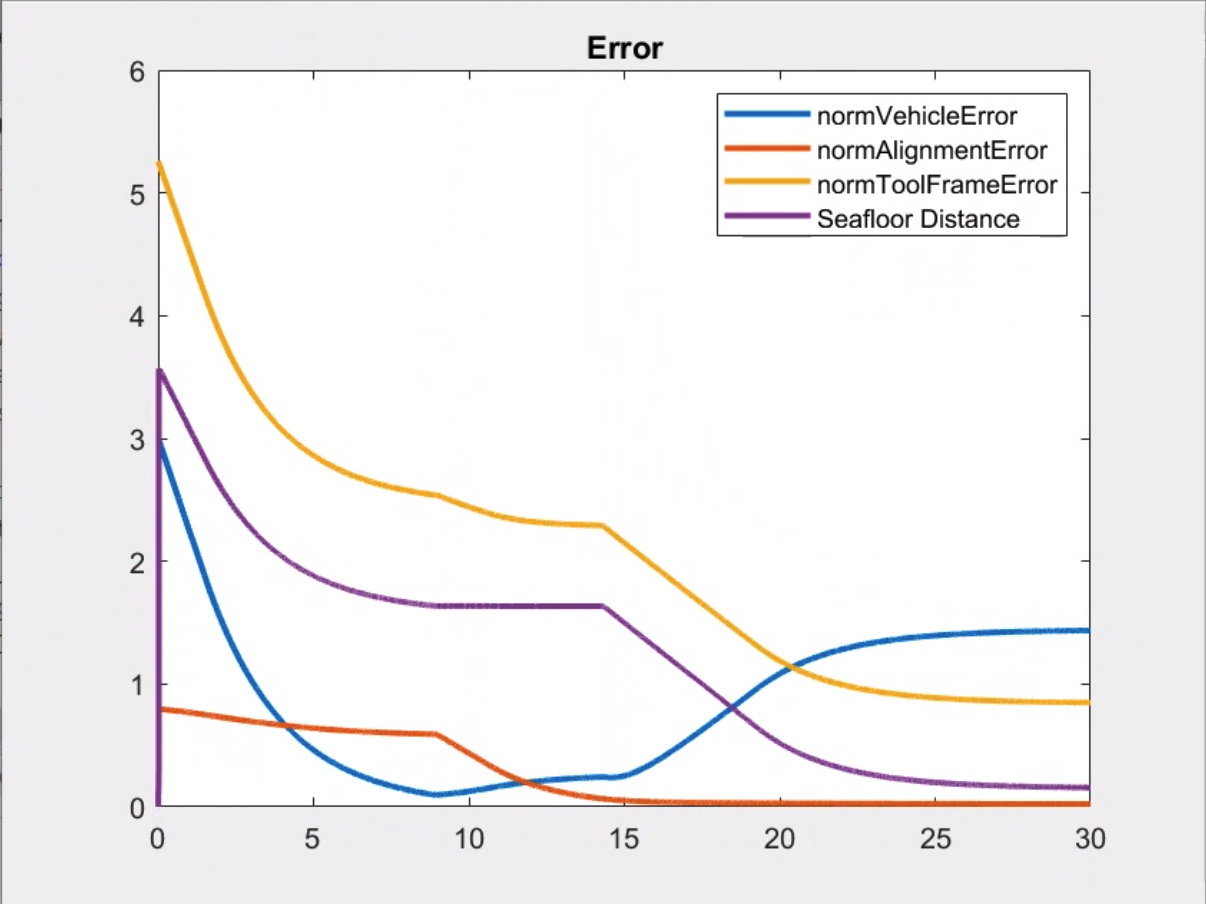
\includegraphics[width=\textwidth]{313_m_Errors.png}
\caption{Errors with medium}\label{err_w_m} 
\end{minipage} 
\hspace{0.2\textwidth} 
\begin{minipage}{0.40\textwidth}  
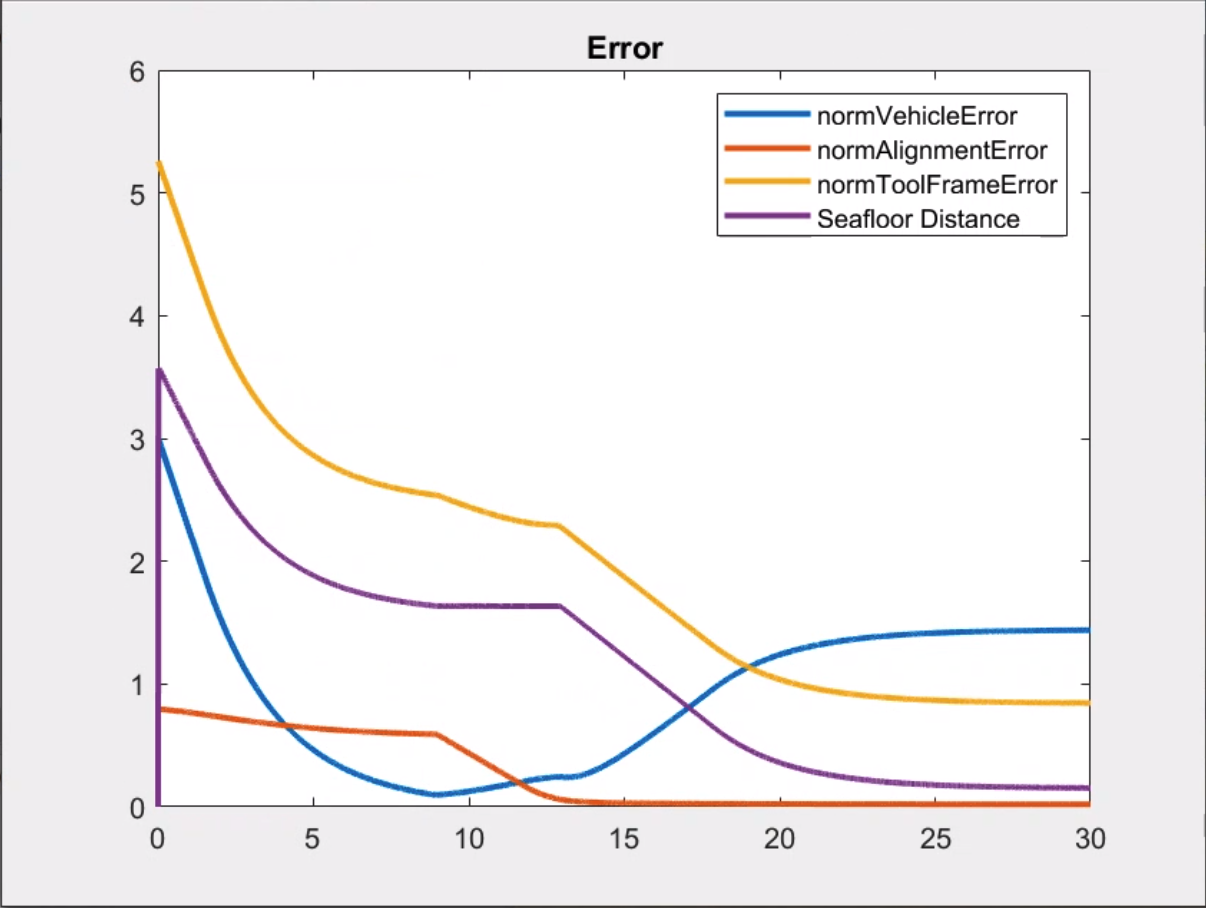
\includegraphics[width=\textwidth]{313_b_Errors.png}
\caption{Errors with big}\label{err_w_b} 
\end{minipage}
\end{figure}
%%%%%%%% MINI PAGE IMAGES %%%%%%%%

\clearpage 
\subsubsection{Q4: After the landing is accomplished, what happens if you try to move the end-effector? Is the distance to the nodule sufficient to reach it with the end-effector? Comment the observed behavior.}\label{ex3}
The tool could reach the center of the nodule, however, we notice that the vehicle moves to ``help'' the arm to achieve the desired position. It is clear that, to avoid this problem, we need to perform a non-reactive task to constraint the vehicle not move, as we will do in the next exercise \ref{subsec:non-react}. 

\begin{figure}[h]
    \centering
    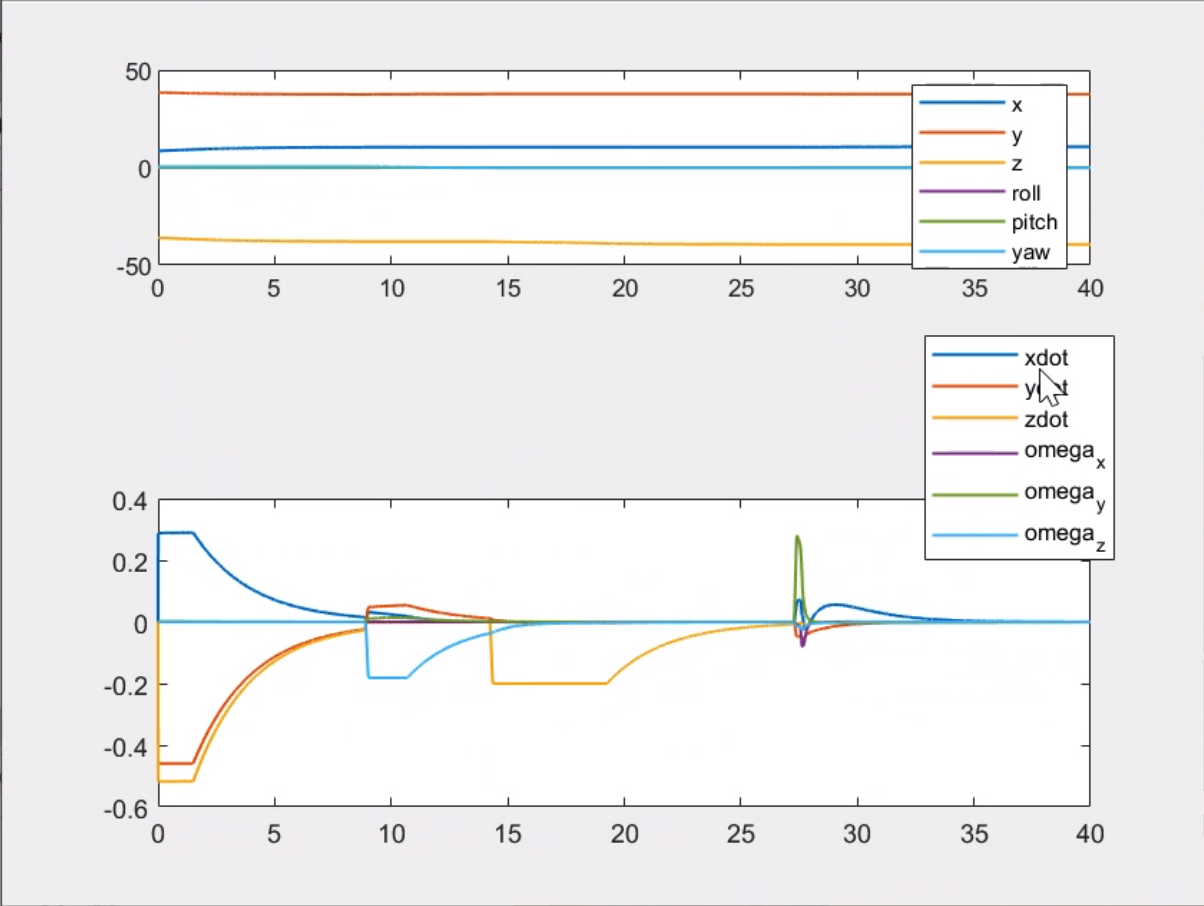
\includegraphics[scale=0.4]{314_ppdot.png}
    \caption{Visible that when tool starts move, vehicle helps it}
    \label{graphes3}
\end{figure}

\clearpage
\section{Exercise 4: Implementing a Fixed-base Manipulation Action}
\subsection{Adding non-reactive tasks} \label{subsec:non-react}
To manipulate as a fixed based manipulator, we need to constraint the vehicle to not move, otherwise the tool frame position task will make the vehicle move.

Goal: Add a constraint task that fixes the vehicle velocity to zero. Land on the seafloor. Try reaching the rock position with the end-effector, and observe that the vehicle does not move.

\subsubsection{Q1: Report the unified hierarchy of tasks used and their priorities. At which priority level did you add the constraint task?}
We have four different actions, with this hierarchy and activations:
%%%%%% TABLE %%%%%%%%%
\begin{center}
\begin{tabular}{ | c | c | c | c | c | c |}
\hline
 Control Task & \texttt{Code name} & Action A & Action B & Action C & Action D\\
 \hline
 Vehicle Null Velocity & \texttt{vNull} & Inactive & Inactive & Inactive & Active\\
 Minimum Altitude Vehicle &  \texttt{mav} & Active & Active & Inactive & Inactive \\  
 Manipulabity &  \texttt{mu} & Active & Active & Active & Active  \\
 Horizontal Attitude &  \texttt{ha} & Active & Active & Active & Active\\
 Alignment to the rock & \texttt{alr} & Inactive & Active & Active & Inactive \\
 Landing & \texttt{l} &Inactive & Inactive & Active & Inactive\\
 Tool  &  \texttt{t} & Inactive & Inactive & Inactive & Active\\
 Vehicle Position &  \texttt{v} &Active & Inactive & Inactive & Inactive\\
 \hline
\end{tabular}
\end{center}
%%%%%% TABLE %%%%%%%%%
\begin{description}
\item \textbf{Vehicle Null Velocity} [NR, E, C], it is a constraint task, so it has higher priority than all the other tasks. The goal of the task is to block the motors.
\item \textbf{Tool Position} [R, E, AD], it is an Action Definition task, that enable the arm to reach the tool target position. 
\end{description}

\begin{description}
	\item Action A, safe waypoint navigation with all the safety task activated
	\item Action B, alignment to the nodule with all the safety task activated
	\item Action C, landing and final rotation to be aligned with the rock
	\item Action D, the new one. Here it is enable the new \textit{Vehicle Null Velocity} task, that disable the UVMS' motors, to prevent movement. The only movement will be the extension of the arm to reach the desired target tool position.
\end{description}

%%%%%%% near images %%%%%%% 
\begin{figure}[htp]
\centering
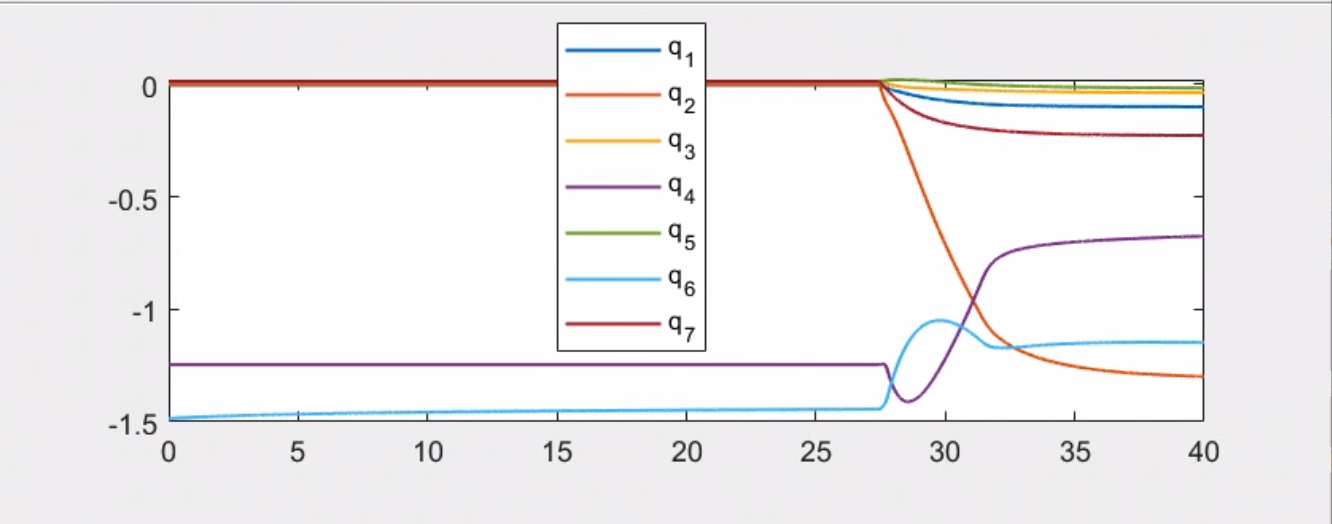
\includegraphics[width=.6\textwidth]{411_q.png}\caption{Arm joints start moving when reached task 4}
\centering
\label{fig:411_arm}
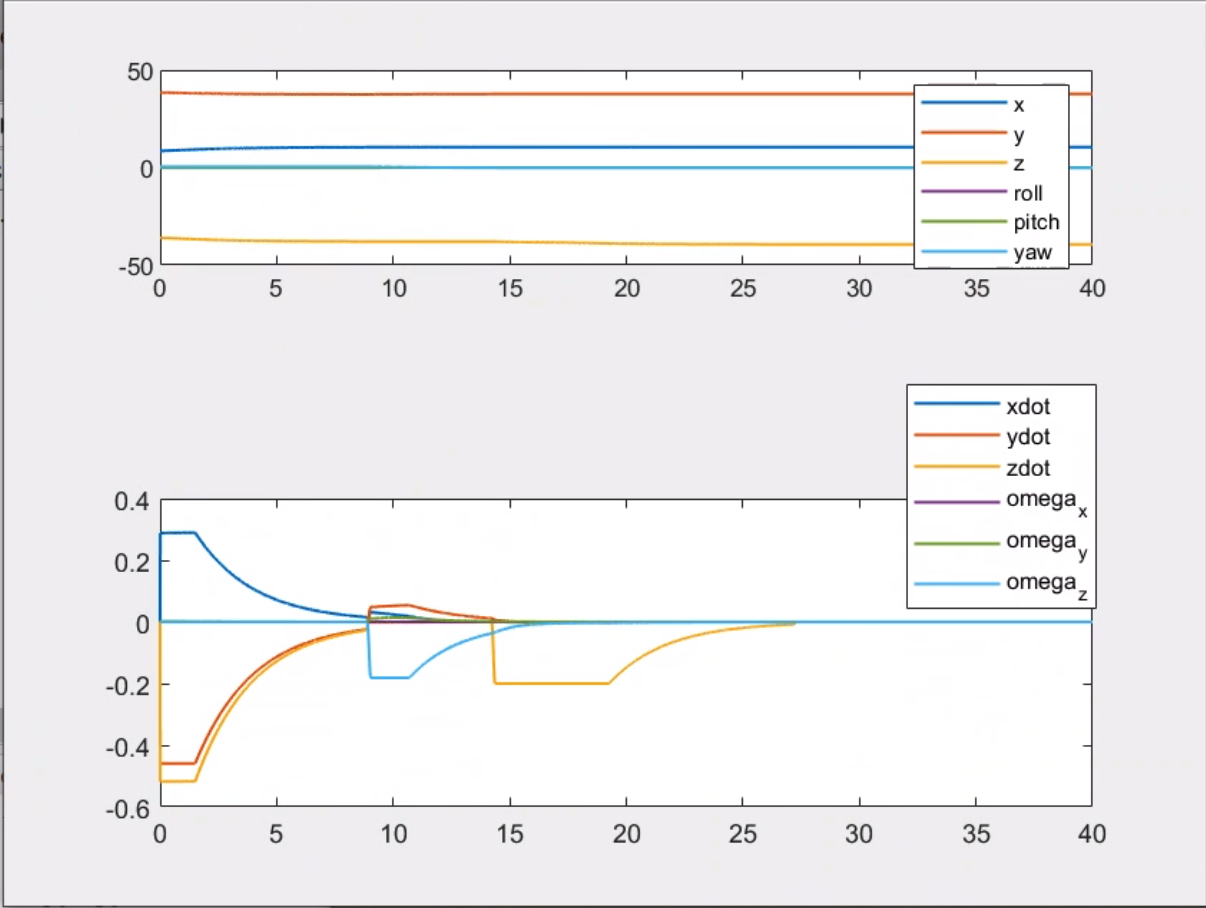
\includegraphics[width=.6\textwidth]{411_ppdot.png}\caption{Vehicle has zero velocities when task 3 is finished}
\label{fig:411_vehicle}
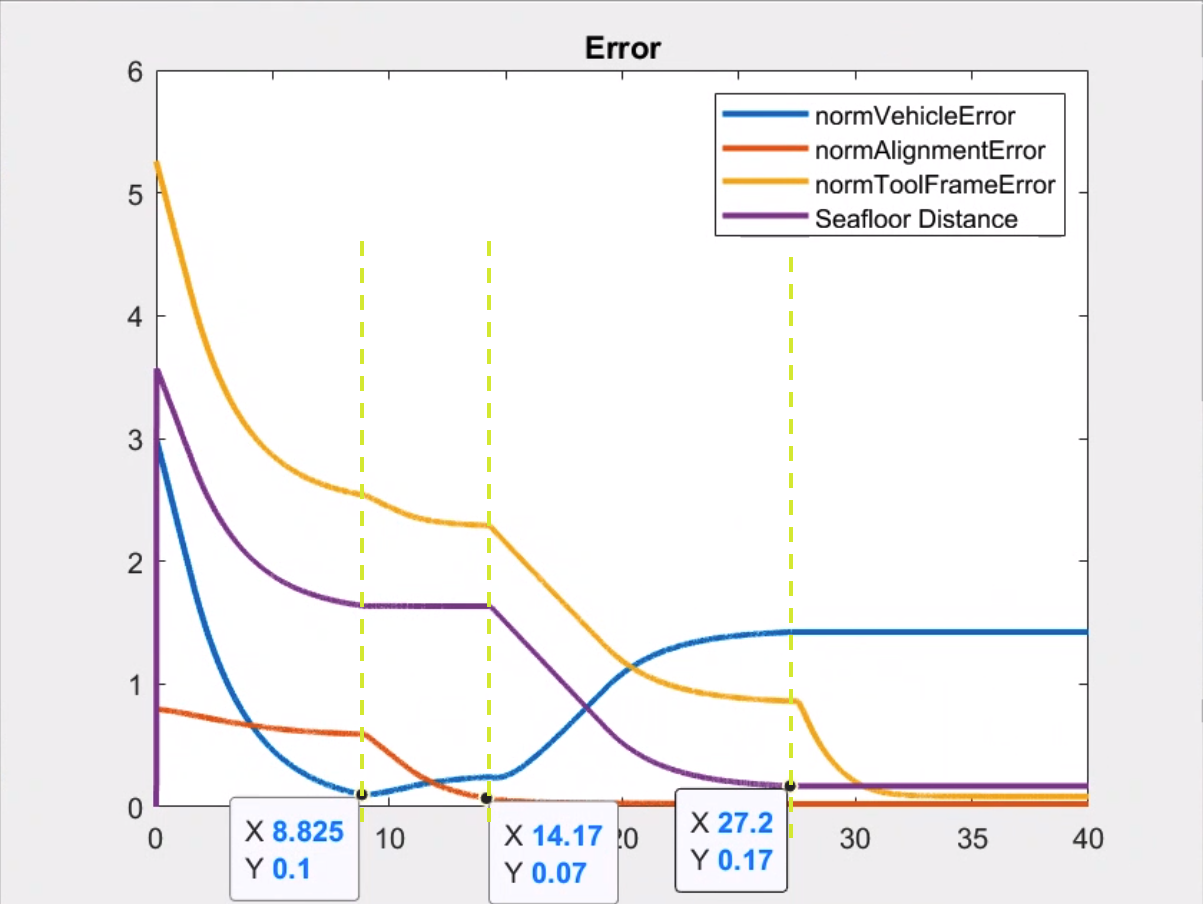
\includegraphics[width=.6\textwidth]{411_Errors.png}\caption{Vehicle has zero velocities when task 3 is finished}
\label{fig:411_errors}
\end{figure}
%%%%%%% %%%%%%%%%% %%%%%%%
\subsubsection{Q2: What is the Jacobian relationship for the Vehicle Null Velocity task? How was the task reference computed?}
The Jacobian for the Vehicle Null Velocity task is the same of the Vehicle Position, but this time we need to fix the velocity of the UVMS to zero, so we premultiply it for the zeros vector. % CI VA IL TRASPOSTO? BE SURE DI OGNI MATRIX COME é FATTA

%%%%%%% Jacobian Matrix %%%%%%% 
\begin{equation}
\large
\boldsymbol{J}_{vehNull}=\begin{bmatrix} 0 & 0 & 0 & 0 & 0 & 0
\end{bmatrix}
    \begin{bmatrix}
     & \underset{3\times 3}{\boldsymbol{0}} & \underset{ 3\times 3}{^{w}\boldsymbol{R}_{v}} \\
     \underset{6\times 7}{\boldsymbol{0}} \\
     & \underset{ 3\times 3}{^{w}\boldsymbol{R}_{v}} & \underset{3\times 3}{\boldsymbol{0}} \\
    \end{bmatrix}
\end{equation}
%%%%%%% %%%%%%% %%%%%%% %%%%%%% 

The velocity will not change during the activation of this task because it is a Non-Reactive.

\subsubsection{Q3: Suppose the vehicle floating, i.e. not landed on the seafloor. What would happen, if due to currents, the vehicle moves?}
The Vehicle Null task cannot take in position the UVMS, it doesn't take into account disturbances, it only put velocities to zero, so it is not able to contrast currents. In this scenario, the robot will start follow the current and it will go to a wrong position. The arm will continue to try to reach the desired position, and because it is not landed, the \textit{Vehicle Null Velocity} is not active, so the Tool Position try to achieve its goal and bring back all the vehicle. If the currents are not too strong it could reach again the position. Different from the previous exercise \ref{ex3}, in which the vehicle could not help the arm to be able to arrive to the target, now it could ``help''. \ocio
\clearpage

\subsection{Adding a joint limit task}
Let us now constrain the arm with the actual joint limits. The vector variables \texttt{uvms.jlmin} and \texttt{uvms.jlmax} contain the maximum and minimum values respectively.

Goal: Add a joint limits avoidance task. Land on the seafloor. Try reaching the rock position with the end-effector, and observe that the vehicle does not move and that all the joints are within their limits.

\subsubsection{Q1: Report the unified hierarchy of tasks used and their priorities. At which priority level did you add the constraint task?}
We have four different actions, with this hierarchy and activations:
%%%%%% TABLE %%%%%%%%%
\begin{center}
\begin{tabular}{ | c | c | c | c | c | c |}
\hline
 Control Task & \texttt{Code name} & Action A & Action B & Action C & Action D\\
 \hline
 Vehicle Null Velocity & \texttt{vNull} & Inactive & Inactive & Inactive & Active\\
 Joint Limit & \texttt{jl} & Active & Active & Active & Active \\
 Minimum Altitude Vehicle &  \texttt{mav} & Active & Active & Inactive & Inactive \\  
 Manipulabity &  \texttt{mu} & Active & Active & Active & Active  \\
 Horizontal Attitude &  \texttt{ha} & Active & Active & Active & Active\\
 Alignment to the rock & \texttt{alr} & Inactive & Active & Active & Inactive \\
 Landing & \texttt{l} &Inactive & Inactive & Active & Inactive\\
 Tool  &  \texttt{t} & Inactive & Inactive & Inactive & Active\\
 Vehicle Position &  \texttt{v} &Active & Inactive & Inactive & Inactive\\
 \hline
\end{tabular}
\end{center}
%%%%%% TABLE %%%%%%%%%

\begin{description}
\item \textbf{Joint Limit} [R, I, S], it is a safety task, so it has higher priority than the other action-defining tasks. It is able to control that the joints don't operate over their prefixed threshold. \ocio
\end{description}

The actions are the same as before, the only difference is that Joint Limit is always active because it is a safety task. However, it is important when the robot perform the final action. 

\subsubsection{Q2: What is the Jacobian relationship for the Joint Limits task? How was the task reference computed?}
The Jacobian for the Joint Limit task is:
%%%%%%% Jacobian Matrix %%%%%%% 
\begin{equation}
\large
\boldsymbol{J}_{jointLimit}=
    \begin{bmatrix}
     \underset{7\times 7}{\boldsymbol{I}} & \underset{7\times6}{\boldsymbol{0}} \\
    \end{bmatrix}
\end{equation}
%%%%%%% %%%%%%% %%%%%%% %%%%%%% 
With this Jacobian we are sure that each joint apply the limit constraints only itself and not on the other ones.
\\
We compute the \textbf{task reference} as:
Seen that each joint influences obviously only itself for the joint limit task.\\
%%%%%%%%%%%%	
\begin{equation}
\large
\dot{\overline{x}}_{jointLimit,i} =k \left\{\begin{array}{ll}
x_{activationMin,i}-x_{q, i} & \text { if } x_{q, i} \leq mid_{i} \\
x_{activationMax,i}-x_{q, i} & \text { if } x_{q, i}>mid_{i}
\end{array}\right.
\end{equation}
%%%%%%%%%%%%%
	where:
	\begin{description}
		\item $i = 1,\dots,7$ is the $i$-th joint.
		\item $x_{q,i}$ is the $i$ joint position ($q$)
		\item $ActivationMin$ and $ActivationMax$ are the $10\%$ of the limit imposed for each joint.
		\item $mid_i = \dfrac{x_{ActivationMin,i} + x_{ActivationMax,i}}{2}\; $ is the middle point between the Minimum Activation and the Maximum.
		\item $k$ is the gain
\end{description}
We use the Min and Max in order to be able to activate the joint limit when the joint arrives near the minimum guard ($ActivationMin$) or near the maximum ones ($ActivationMax$).
%%%%%%%%
\clearpage

\section{Exercise 5: Floating Manipulation}
\subsection{Adding an optimization control objective}
Use the DexROV simulation for this exercise .

The goal is to try to optimize the joint positions, if possible, to keep the first four joints in a "preferred shape", represented by the following vector
\begin{displaymath}
\begin{bmatrix}-0.0031 & 1.2586 & 0.0128 & -1.2460 \end{bmatrix}^\top
\end{displaymath}

Goal: Add an optimization objective to keep the first four joints of the manipulator in the preferred shape. Observe the behaviour with and without the task

\subsubsection{Q1: Report the unified hierarchy of tasks used and their priorities. At which priority level did you add the optimization task?}

The new hierarchy of tasks is:
\begin{itemize} 
	\item Manipulability
	\item Horizontal attitude
        \item Tool
        \item Preferred Shape 
\end{itemize}

\textbf{Preferred Shape [NR, I, O]} is an optimization task. For this reason, it is placed at the end of the hierarchy which means that it has the lowest priority and it is accomplished only if all the other tasks has been already satisfied. 

\subsubsection{Q2: What is the Jacobian relationship for the Joint Preferred Shape task? How was the task reference computed?}

We decided to implement this task as a vector one, thus the Jacobian is a 4-by-13 matrix:
%%%%%%% Jacobian Matrix %%%%%%% 
\begin{equation}
\large
\boldsymbol{J}_{vehNull}=
\begin{bmatrix}-0.0031 & 1.2586 & 0.0128 & -1.2460 \end{bmatrix}^\top
    \begin{bmatrix}
     \underset{4\times4}{\boldsymbol{I}} & \underset{4\times9}{\boldsymbol{0}} \\
    \end{bmatrix}
\end{equation}
%%%%%%%%%%%%%%%%%%%%%%%
The Jacobian has four rows since it is required to control just the first fuor joints. Since each joint affects only itself (similarly to the joint limits task), the non-zero part of the Jacobian is a 4-by-4 identity matrix. 

We compute the \textbf{task reference} as the difference between the desired joint configuration and the actual one :

\begin{equation}
\large
   \dot{\overline{\boldsymbol{x}}}_{prefShape} = k(x_{prefShape} - x_{q}) %delta
\end{equation}
\begin{itemize}
    \item $k$ is the control gain.
    \item $x_{prefShape}$ is the desired configuration of the first four joints.
    \item $x_{q}$ is the actual configuration of the first four joints.
\end{itemize} 

\subsubsection{Q3: What is the difference between having or not having this objective?} %FICCARE COLLEGAMENTO IMMAGINI
In this specific case the UVMS goal is to align the end-effector frame to the goal frame which is located slightly above the pipe. Since no explicit goal for the vehicle was given, we have used just the tool task (which is able to move the vehicle as well) in order reach the goal directly. Nevertheless, since we have just one mission phase the manipulator moves in order to achieve the goal as soon as possible, leading to a "stretched" shape (Figure \ref{513_nh1}). If we add the preferred shape constraint as defined in the above mentioned task, we can maintain the desired end-effector configuration, even with just one mission phase (Figure \ref{513_h1}). As we can see in the figures below (Figure \ref{513_nh2} and Figure \ref{513_h2}), when the preferred shape task is active the joints are in a more natural shape, which is also further from the joint limits.
%%%%%%%%% MINI PAGE IMAGES %%%%%%%%
%\begin{figure}[htp]
%    \centering
%    \begin{minipage}{0.50\textwidth}
%    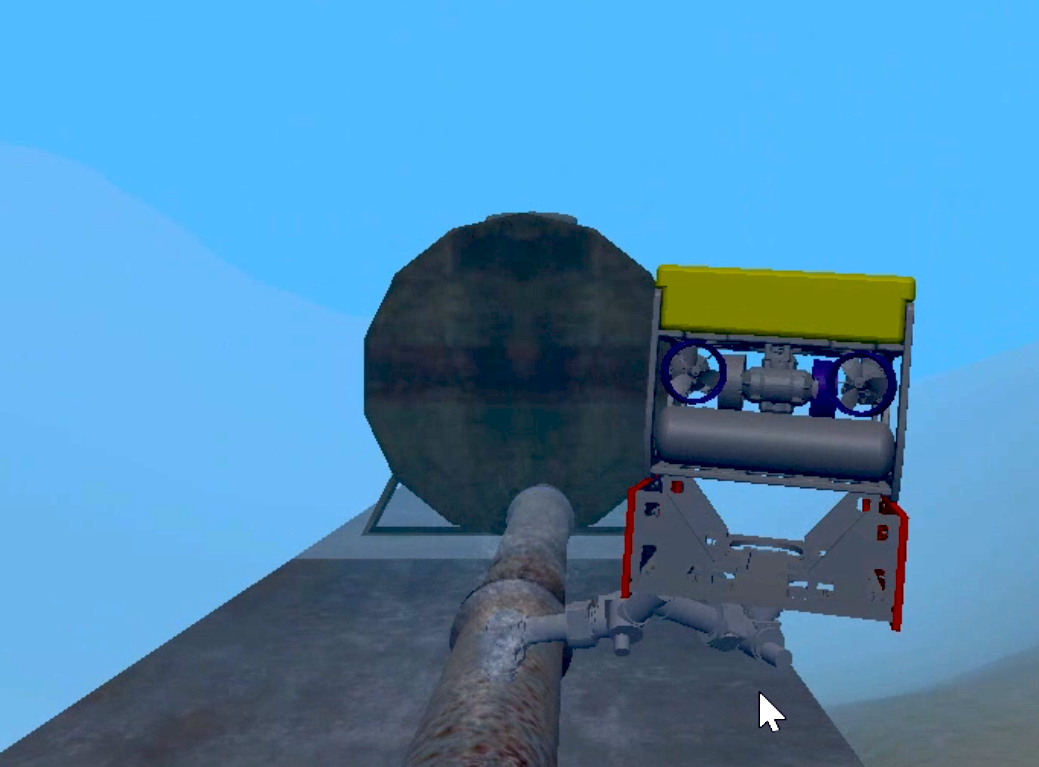
\includegraphics[scale=0.37]{513_comment.png}
%    \caption{Not having}
%    \end{minipage}
%\hfill
%    \centering
%    \begin{minipage}{0.50\textwidth}
%    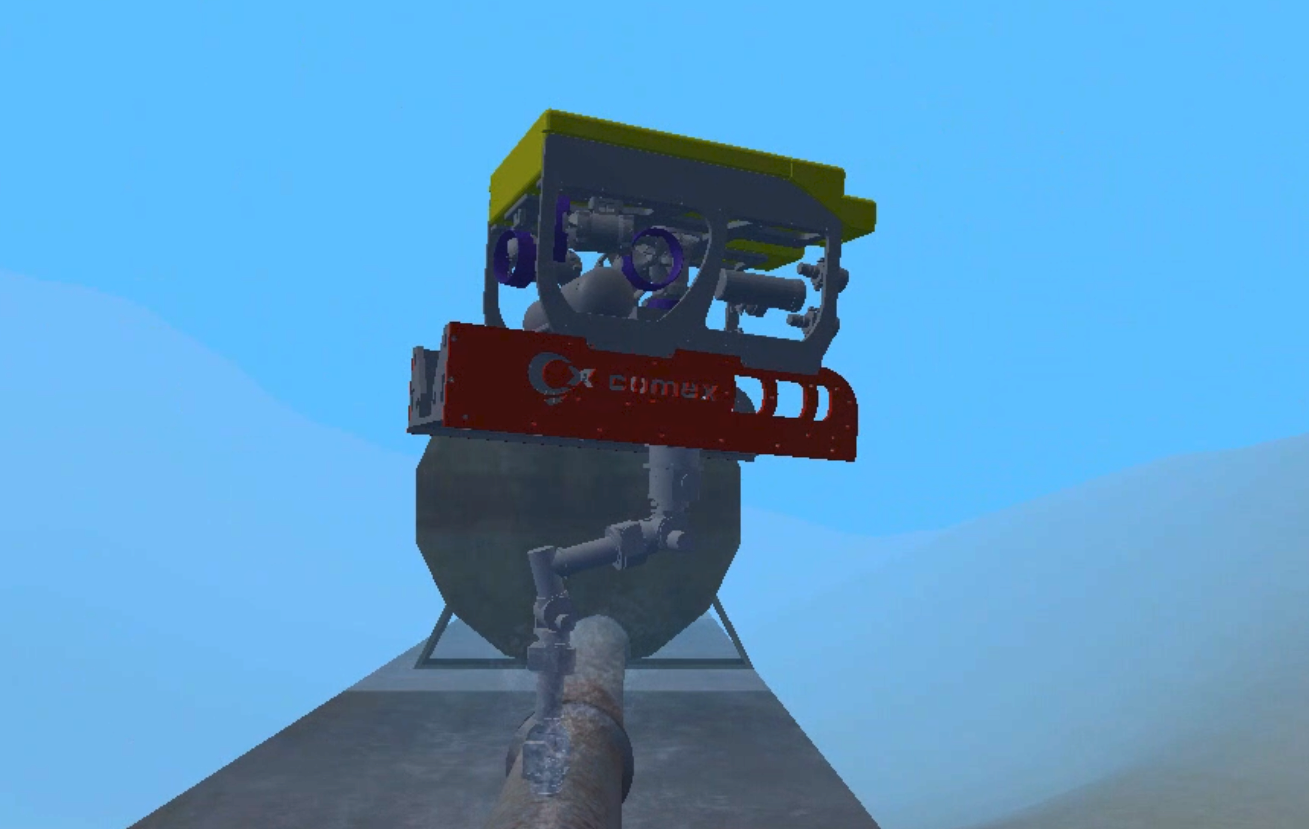
\includegraphics[scale=0.3]{513_uncomment.png}
%    \caption{Having}
%    \end{minipage}
%\end{figure}
%%%%%%%%%%%%%%%%%%%%%%%%%%%%
%\begin{figure}[htp]
%    \centering
%    \begin{minipage}{0.50\textwidth}
%    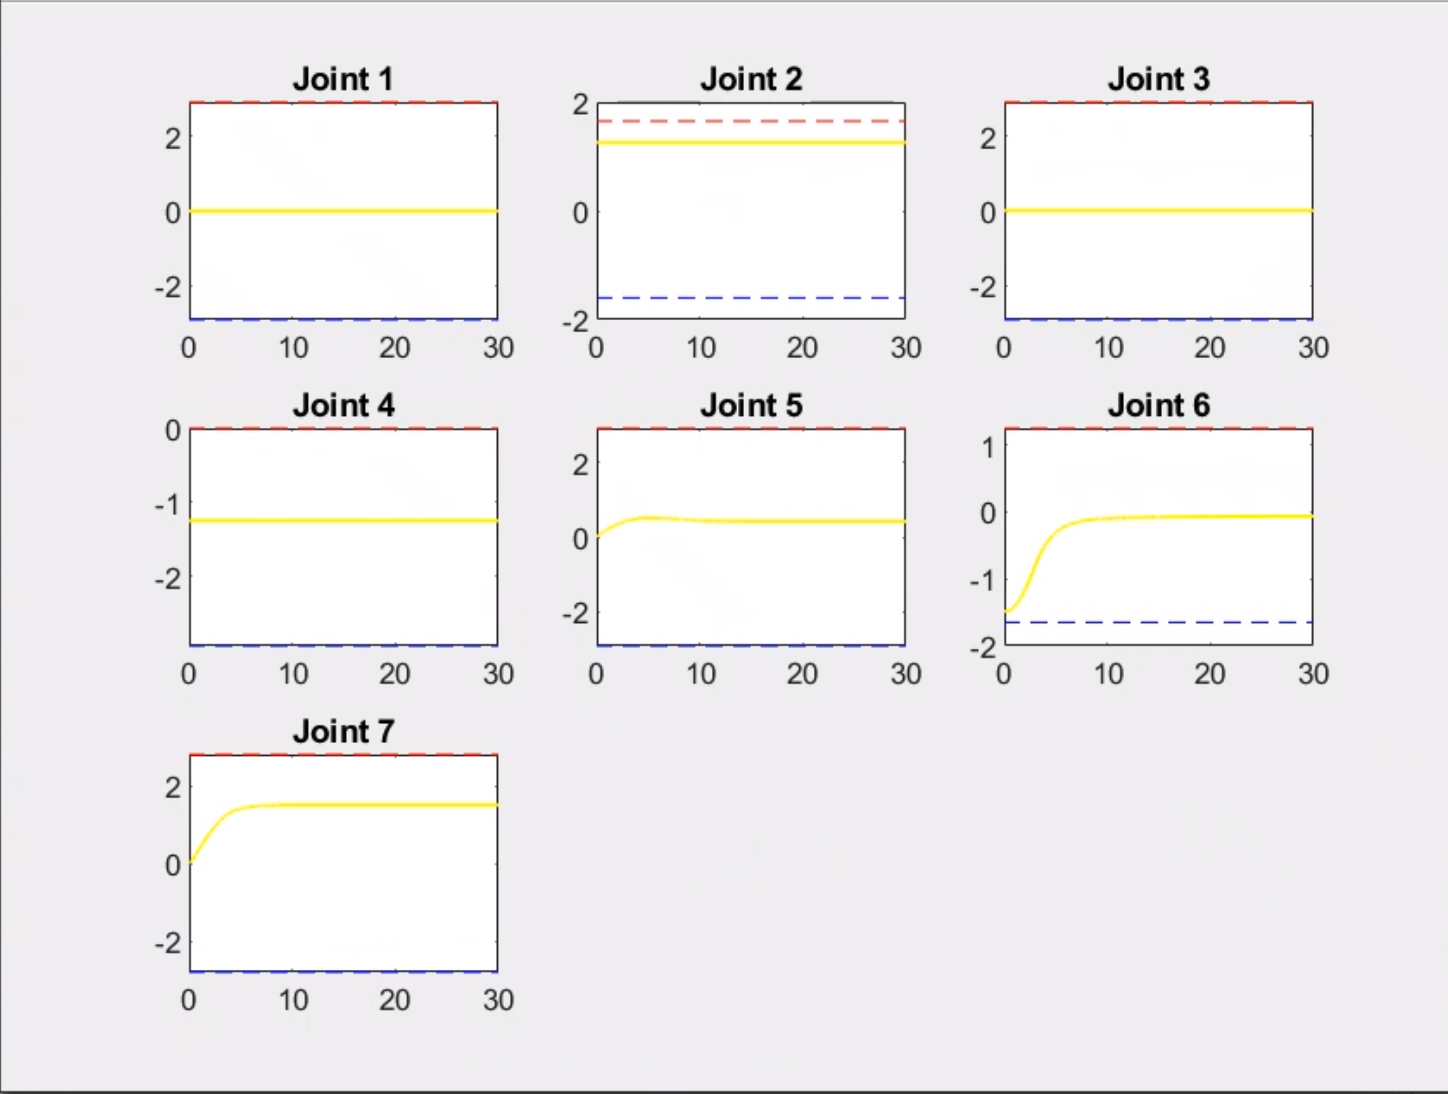
\includegraphics[scale=0.4]{513_jointlimits.png}
%    \caption{Not having}
%    \end{minipage}
%\hfill
%    \centering
%    \begin{minipage}{0.50\textwidth}
%    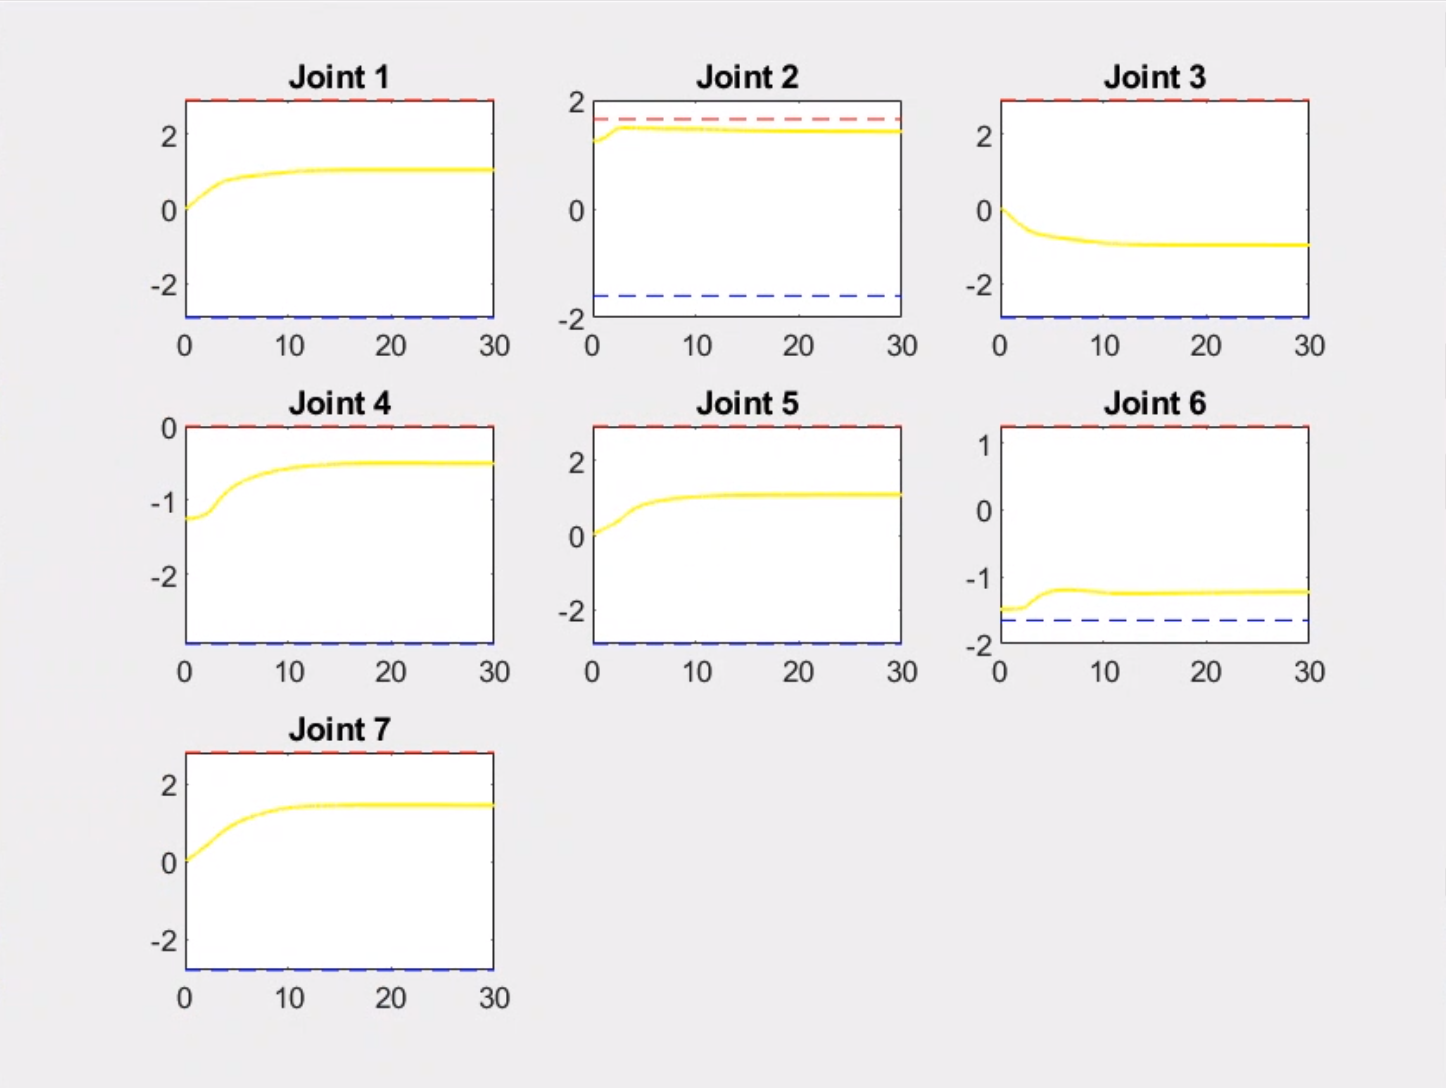
\includegraphics[scale=0.4]{513_woutPS_jointLimits.png}
%    \caption{Having}
%    \end{minipage}
%\end{figure}
%%%%%%%%% MINI PAGE IMAGES %%%%%%%%

\begin{figure}[htpb] 
\begin{minipage}{0.40\textwidth}  
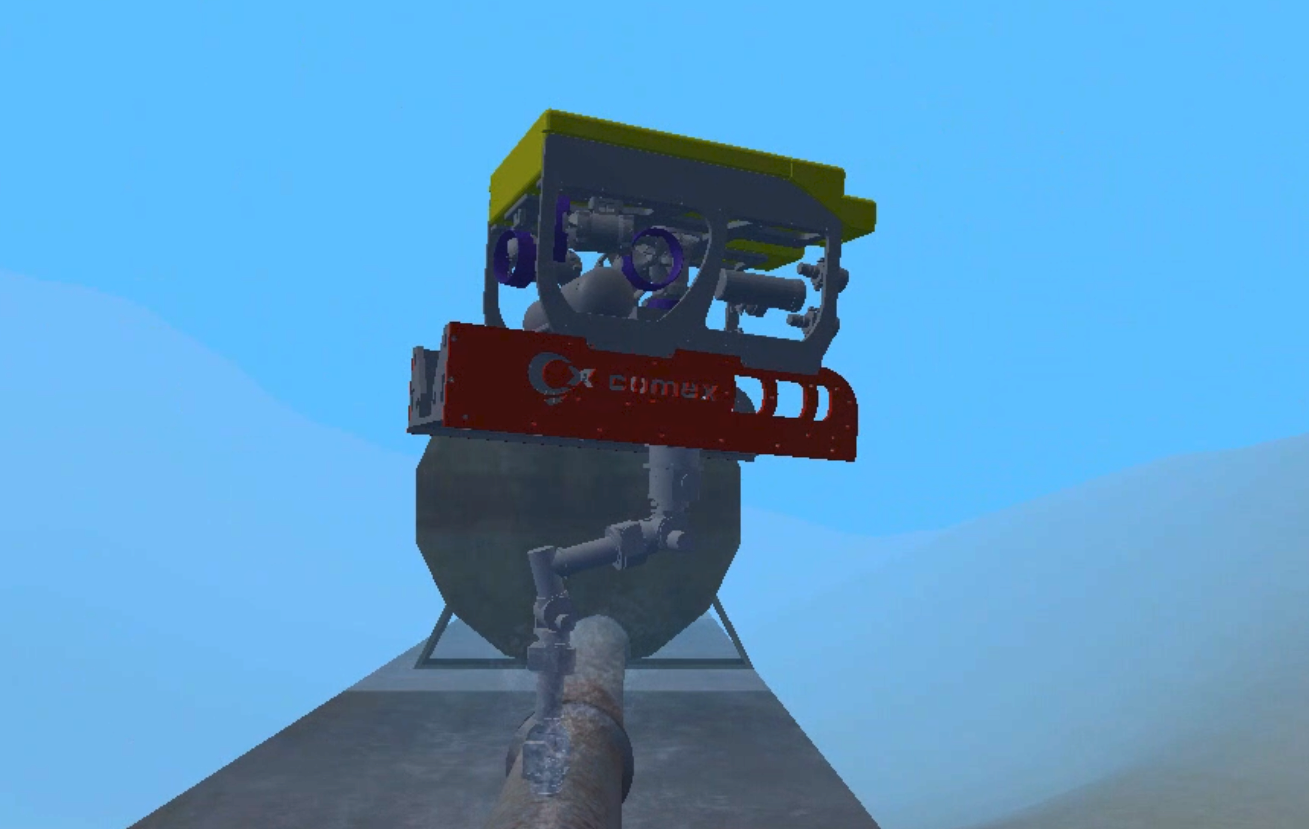
\includegraphics[width=\textwidth]{513_uncomment.png}
\caption{Simulation with Mission Phase}\label{513_nh1} 
\end{minipage}  
\hspace{0.2\textwidth} 
\begin{minipage}{0.40\textwidth}  
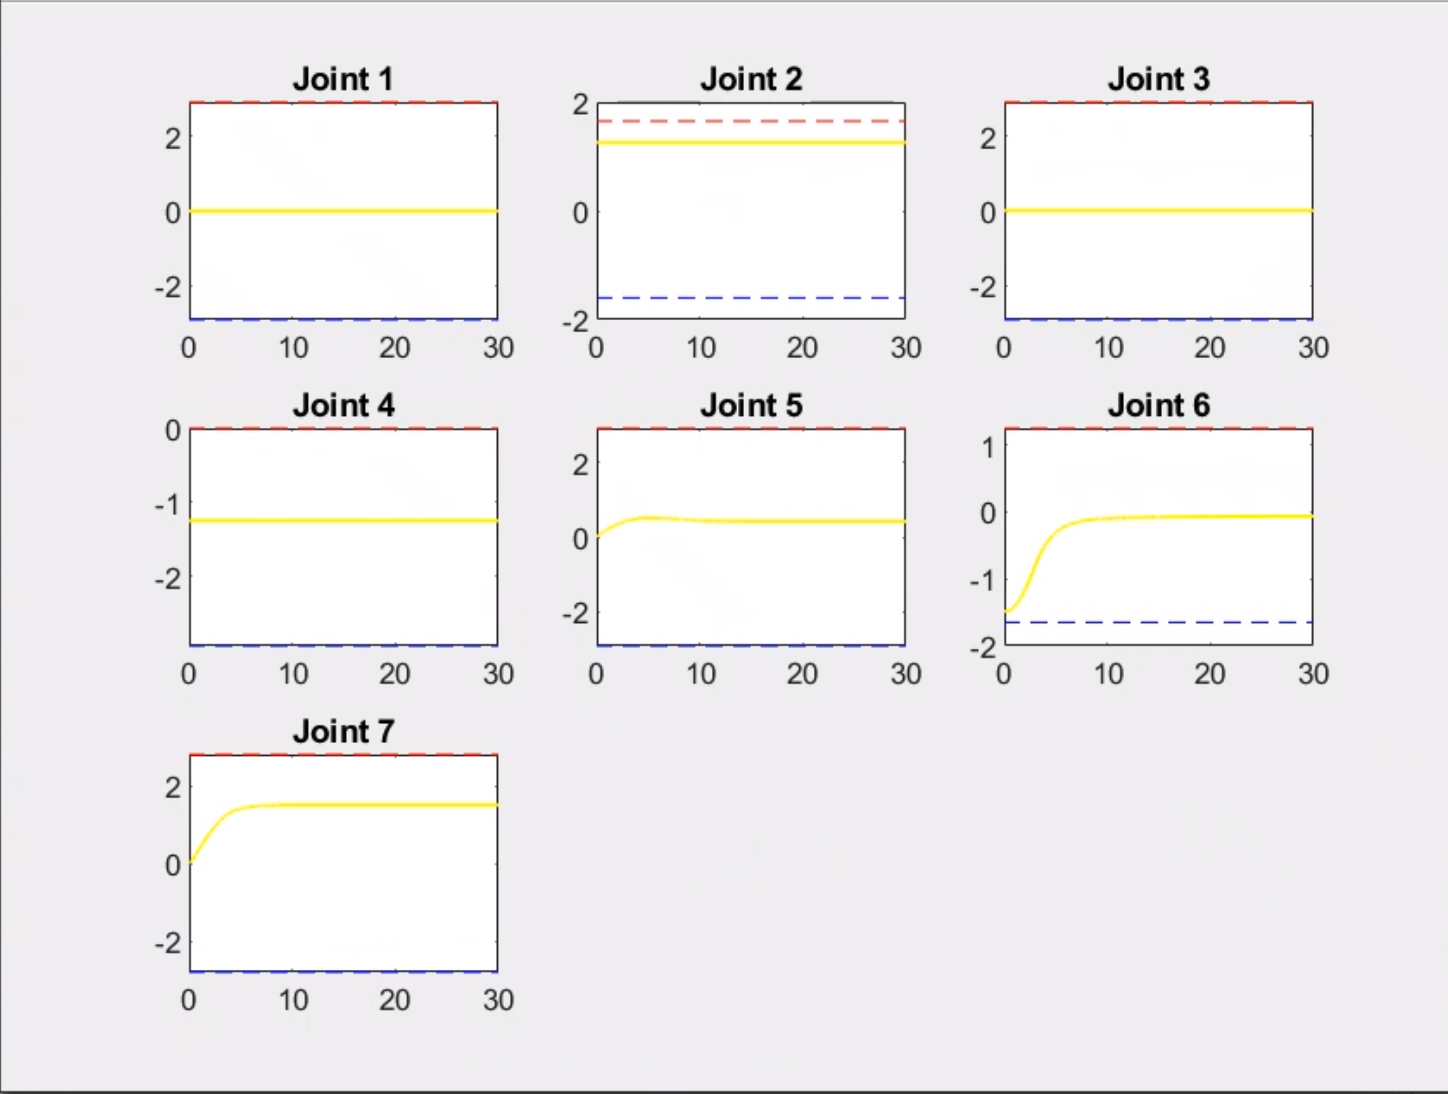
\includegraphics[width=\textwidth]{513_jointlimits.png}
\caption{Joints Limits with Mission Phase}\label{513_h1} 
\end{minipage} 
\hspace{0.2\textwidth} 
\begin{minipage}{0.40\textwidth}  
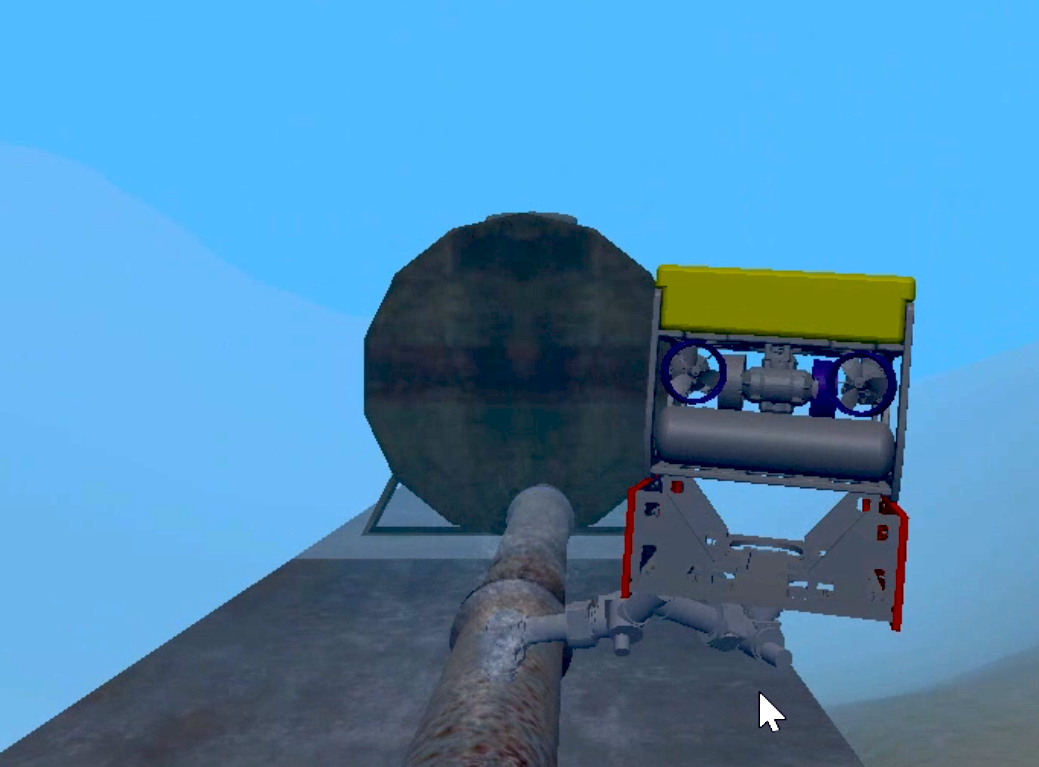
\includegraphics[width=\textwidth]{513_comment.png}
\caption{Simulation without Mission Phase}\label{513_nh2} 
\end{minipage}
\hspace{0.2\textwidth} 
\begin{minipage}{0.40\textwidth}  
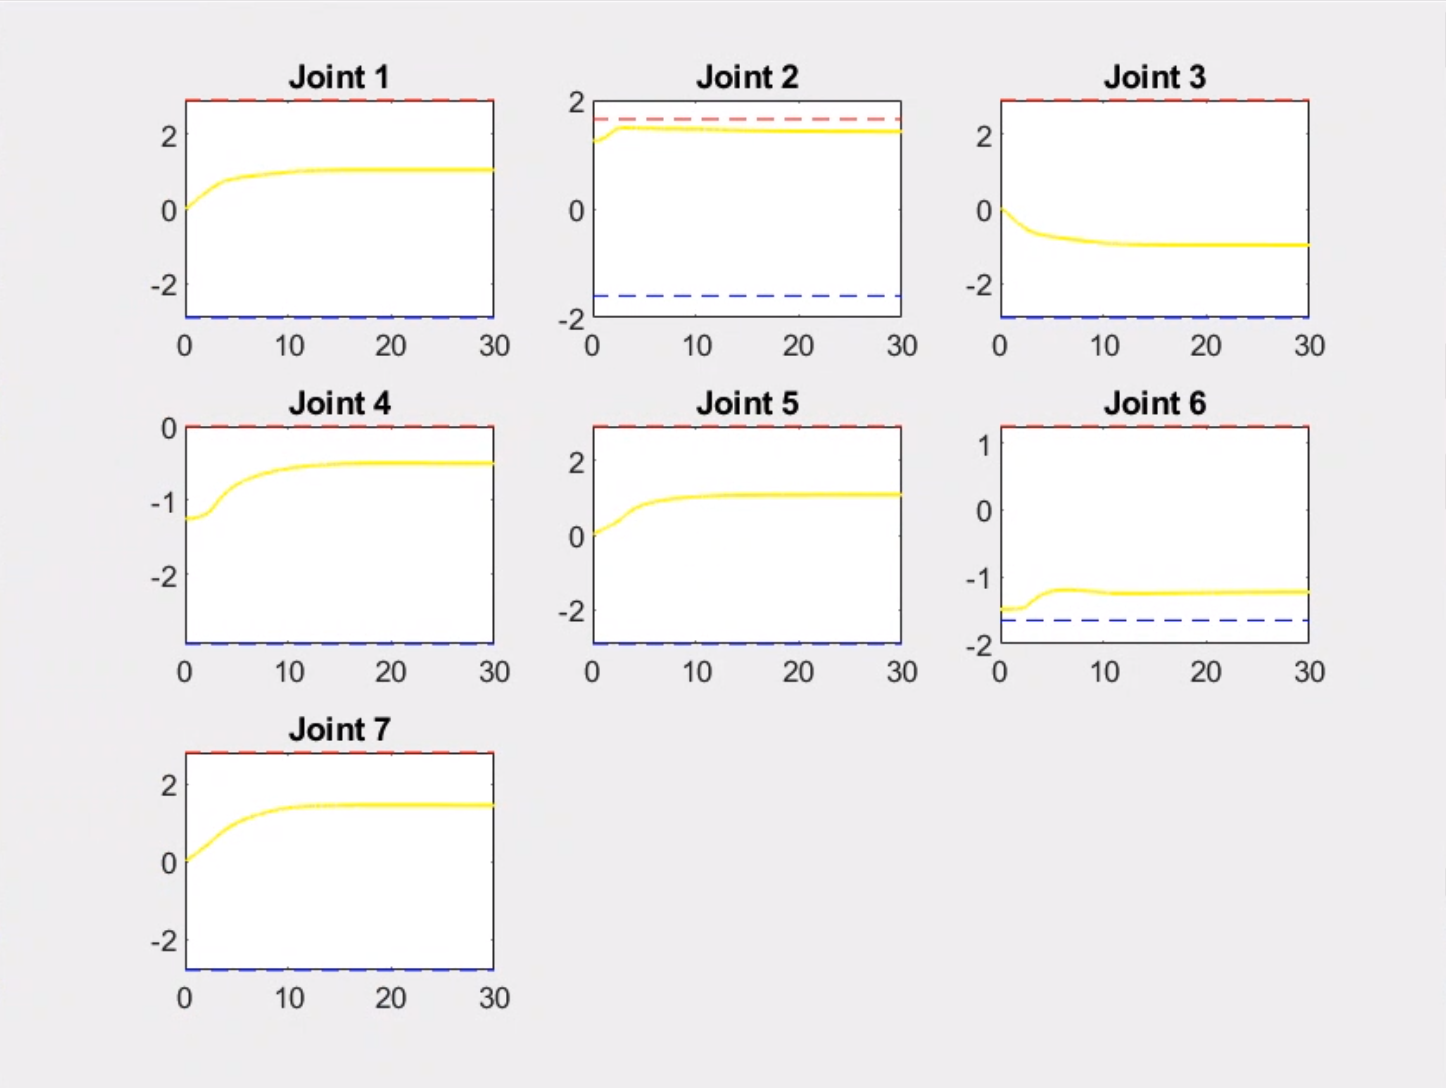
\includegraphics[width=\textwidth]{513_woutPS_jointLimits.png}
\caption{Joints Limits without Mission Phase}\label{513_h2} 
\end{minipage}
\end{figure}


\clearpage

\subsection{Adding mission phases}
Let us now structure the mission in more than one phase. In the first phase, exploit the previous exercises, and implement a safe waypoint navigation. Move the vehicle to a location close to the current defined end-effector goal position, just slightly above it. Then, trigger a change of action and perform floating manipulation.

Goal: introduce mission phases in the floating manipulation scenario. Observe the difference.

\subsubsection{Q1: Report the unified hierarchy of tasks used and their priorities. Which task is active in which phase/action?}

%%%%%% TABLE %%%%%%%%%
\begin{center}
\begin{tabular}{ | c | c | c | c |}
\hline
 Control Task & \texttt{Code name} & Action A & Action B \\
 \hline
 Vehicle Null Velocity & \texttt{vNull} & Inactive & Active \\
 Joint Limit & \texttt{jl} & Active & Active \\
 Manipulabity &  \texttt{mu} & Active & Active\\
 Horizontal Attitude &  \texttt{ha} & Active & Active \\
 Tool  &  \texttt{t} & Inactive & Active\\
 Vehicle Position &  \texttt{v} &Active & Inactive\\
 Preferred Shape & \texttt{ps} & Active & Active\\
 \hline
\end{tabular}
\end{center}
%%%%%% TABLE %%%%%%%%%

% FICCARE IMMAGINI
\subsubsection{Q2: What is the difference with the previous simulation (still in exercise 5), where only one action was used?}
In the previous simulation it was not possible to constrain the vehicle velocities to zero, in order to allow a safe manipulation. By adding a safe navigation phase it is possible to use the vehicle position task to move the UVMS to a position slightly above the pipe, then constrain vehicle velocities in order to allow the manipulator to reach the goal frame by activating the tool task. Moreover, this results in a smoother behavior as it shown in the figures below (Figure \ref{522_n1} and \ref{522_n2}).

%%%%%%%% MINI PAGE IMAGES %%%%%%%%

%\begin{figure}[htp]
%    \centering
%    \begin{minipage}{0.50\textwidth}
%    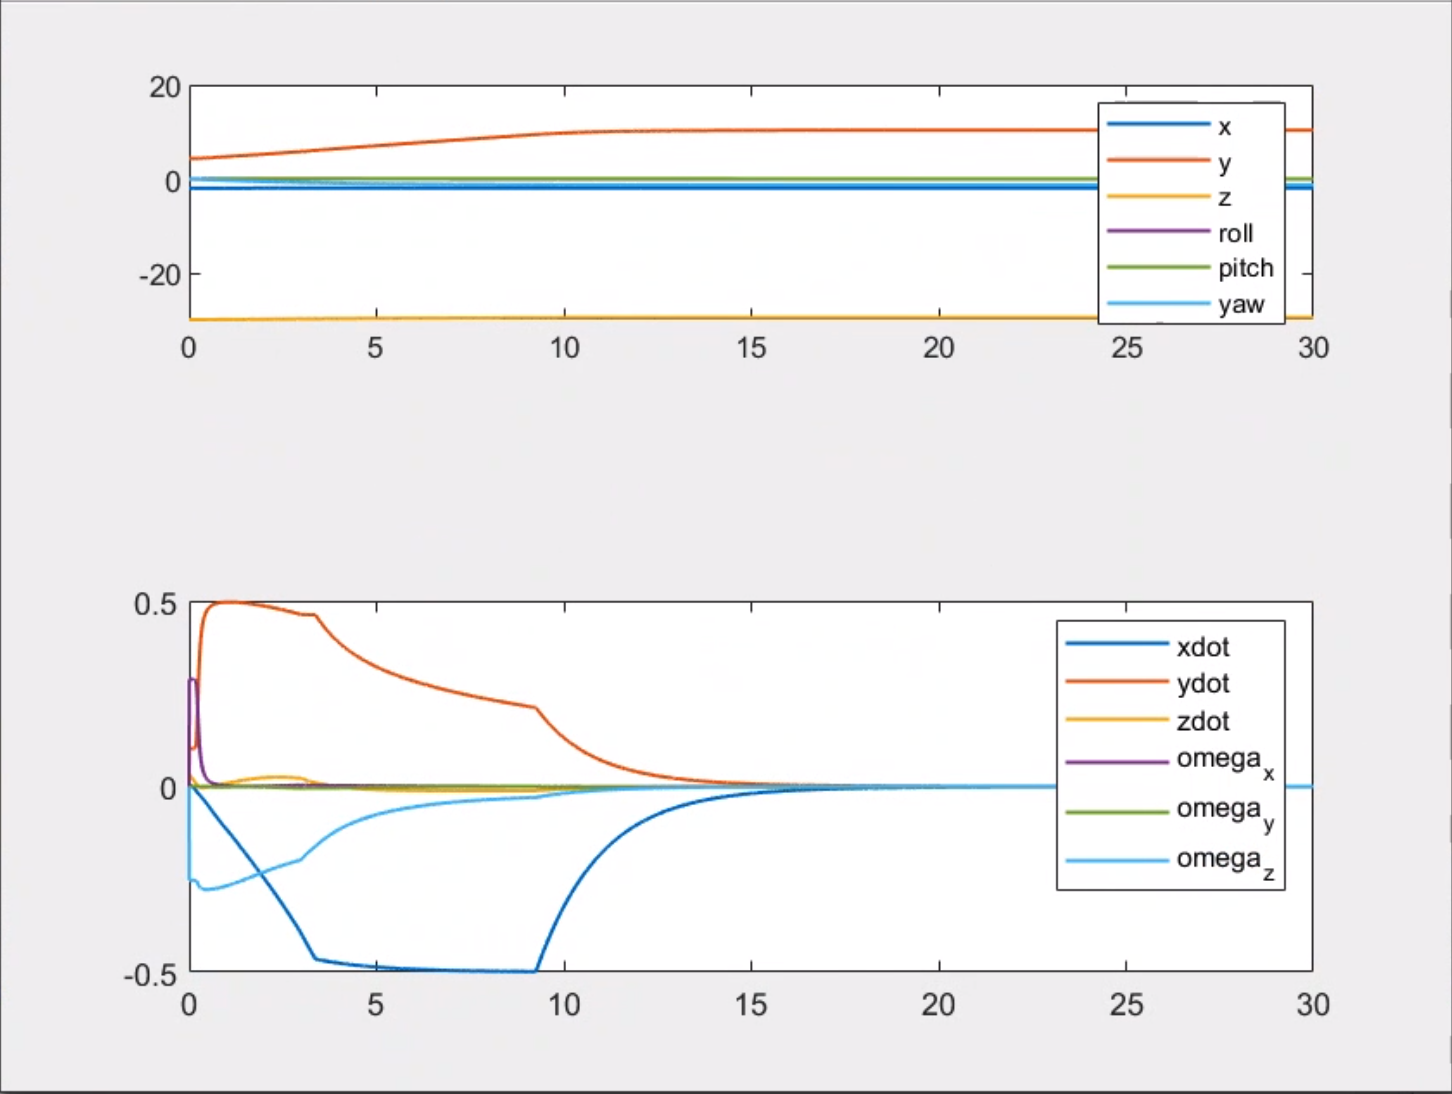
\includegraphics[scale=0.4]{522_wout_MP.png}
%    \caption{Not having}
%    \end{minipage}
%\hfill
%    \centering
%    \begin{minipage}{0.50\textwidth}
%    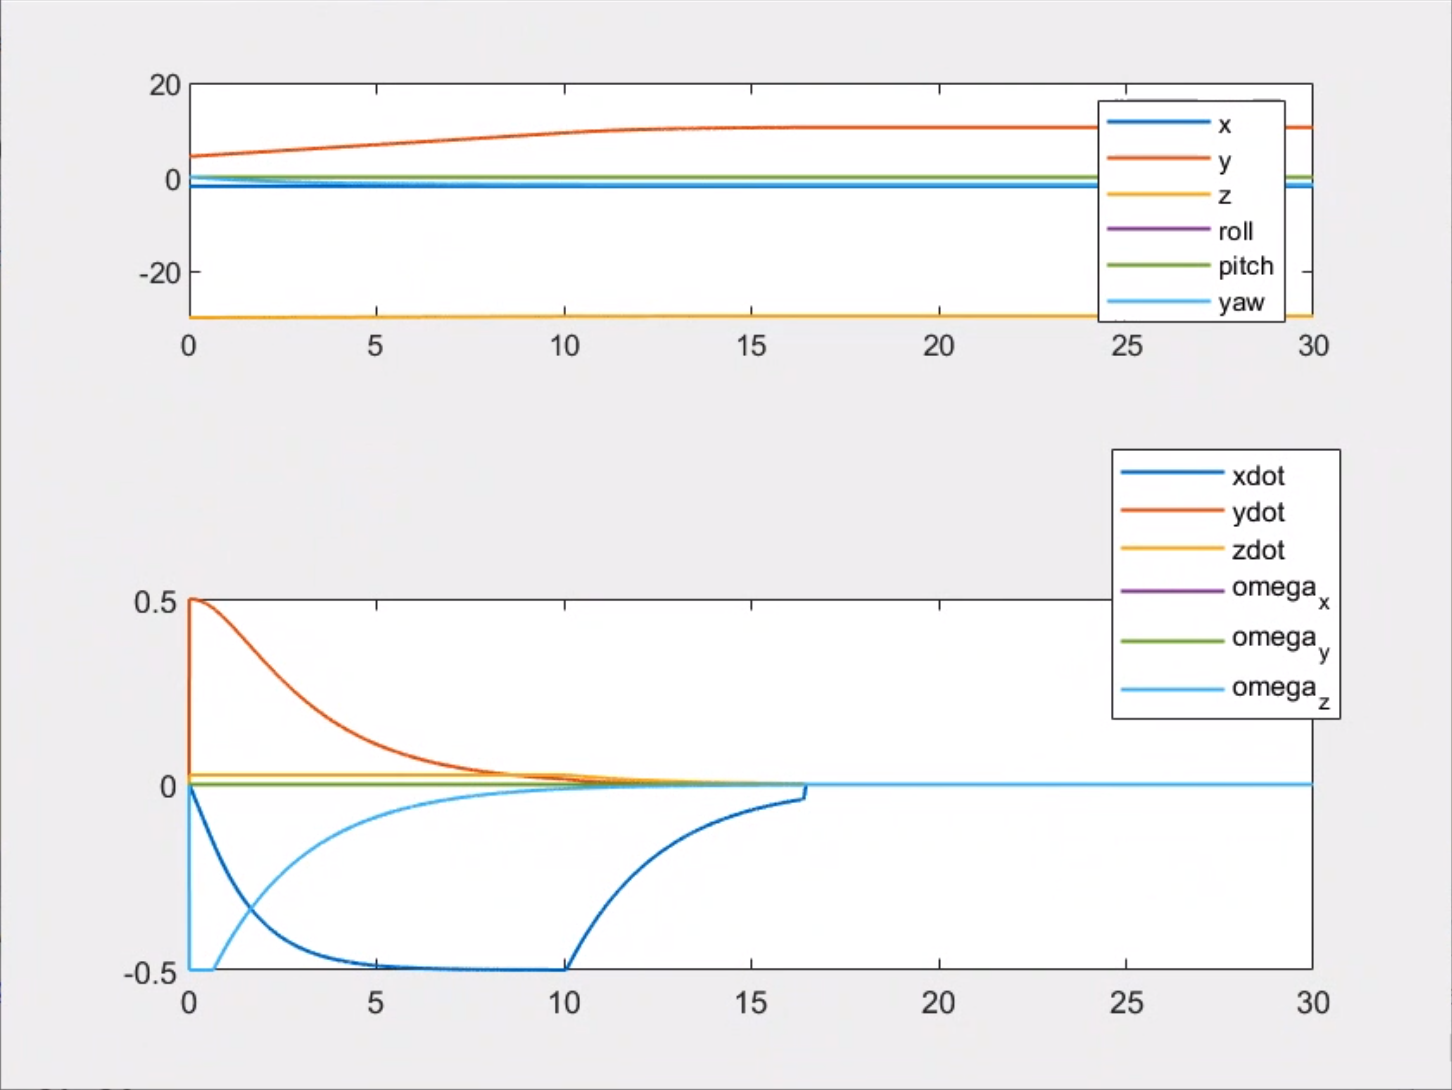
\includegraphics[scale=0.4]{522_w_MP.png}
%    \caption{Having}
%    \end{minipage}
%\end{figure}

%%%%%%%% MINI PAGE IMAGES %%%%%%%%

\begin{figure}[htpb] 
\begin{minipage}{0.40\textwidth}  
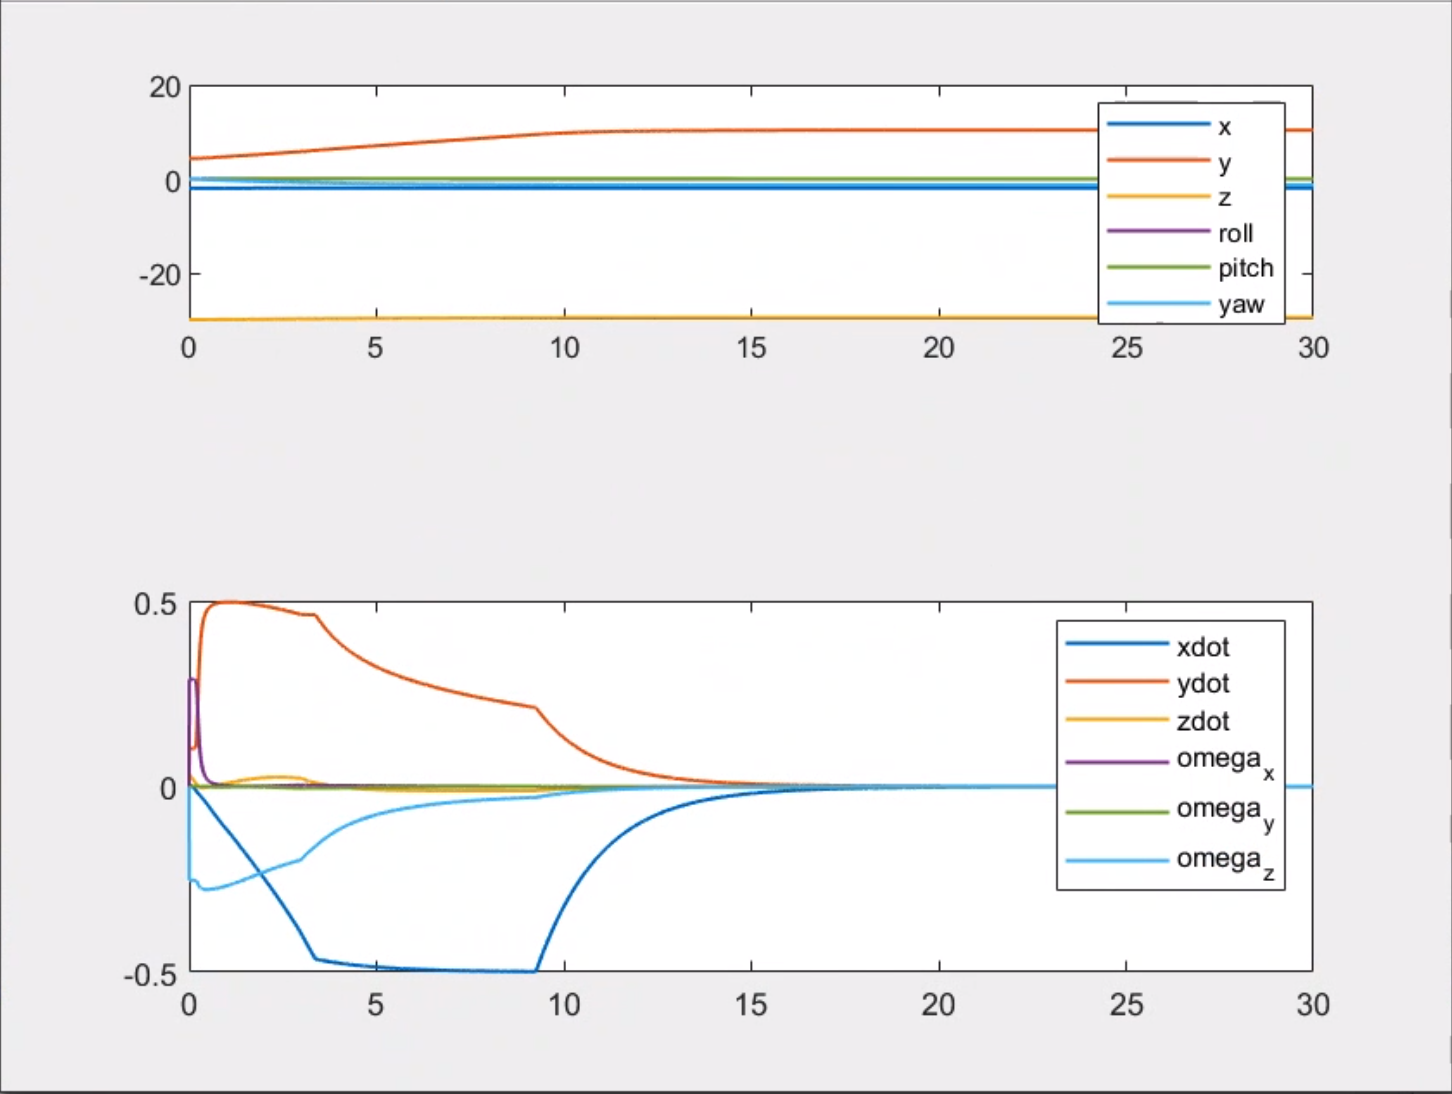
\includegraphics[width=\textwidth]{522_wout_MP.png}
\caption{Simulation with Mission Phase}\label{522_n1} 
\end{minipage}  
\hspace{0.2\textwidth} 
\begin{minipage}{0.40\textwidth}  
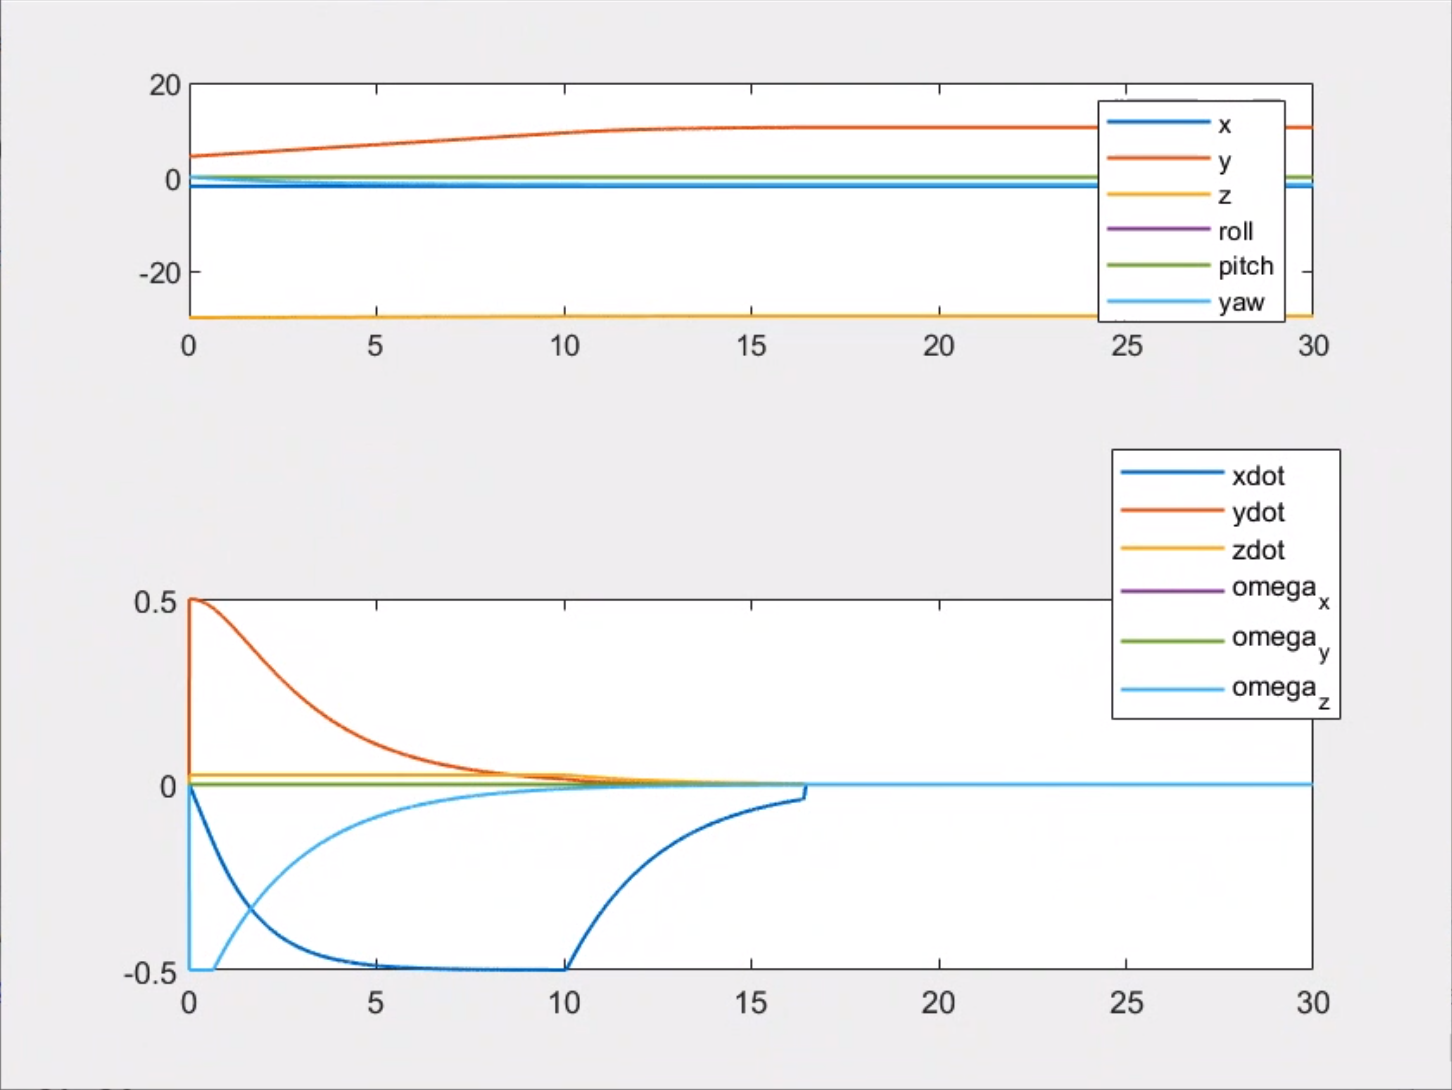
\includegraphics[width=\textwidth]{522_w_MP.png}
\caption{Joints Limits with Mission Phase}\label{522_n2} 
\end{minipage} 
\end{figure}
\clearpage
\section{Exercise 6: Floating Manipulation with Arm-Vehicle Coordination Scheme}
\subsection{Adding the parallel arm-vehicle coordination scheme}
Let us now see how the two different subsystems (arm and vehicle) can be properly coordinate. Introduce in the simulation a sinusoidal velocity disturbance acting on the vehicle, and assume the actual vehicle velocity measurable. To do so, add a constant (in the inertial frame) velocity vector to the reference vehicle velocity before integrating it in the simulator. 

Goal: modify the control part to implement the parallel arm-vehicle coordination scheme. Observe that, even with a disturbance acting on the vehicle, the end-effector can stay in the required constant position.

\subsubsection{Q1: Which tasks did you introduce to implement the parallel coordination scheme?}
In order to implement an arm-vehicle coordination scheme, we implemented two optimizations (TPIK1 and TPIK2) running in parallel. Given an action $A$ the scheme works as follow:

\begin{enumerate}
\item TPIK1 is the same of the previous exercises. It considers the vehicle and the manipulator as a fully controllable system. Therefore, when the hierarchy of task corresponding to the action $A$ is solved, we take the reference for the vehicle velocities while we discard the joints velocities one.
\item TPIK2 is equal to TPIK1 plus an additional task at the top of the hierarchy. This task is a non-reactive one and it is used to constrain the vehicle velocities. The Jacobian for this task is:
\begin{equation}
\large
\boldsymbol{J}_{vConstr}=
    \begin{bmatrix}
     \underset{6\times7}{\boldsymbol{0}} & \underset{6\times6}{\boldsymbol{I}} \\
    \end{bmatrix}
\end{equation}
Its reference is the vector of the vehicle velocities computed by TPIK1 at the previous step. In a real world case, the reference would be the vector of the measured vehicle velocities, but, since we are working in a simulation environment, we are allowed to use the ones computed by the algorithm in the previous loop iteration.
Therefore, TPIK2 provides the optimal joints velocities by taking into account the "real" movement of the vehicle, which is different from the one computed by the algorithm because of the sinusoidal disturbance.
\end{enumerate}

\subsubsection{Q2: What happens if the sinusoidal disturbance becomes too big?}
The vehicle and the manipulator try to compensate the disturbances. This means that if the gain is high enough and the amplitude of the disturbance is not too big, they are fast enough to reduce the error at the price of a smooth behaviour. Nevertheless when the amplitude of the sinusoidal disturbance becomes too big, they are not able to follow and to minimize the error, resulting in a sinusoidal behavior visible on the related plot (AGGIUNGERE IMMAGINI)??.
%%%%%%%% MINI PAGE IMAGES %%%%%%%%
\begin{figure}[htpb] 
\begin{minipage}{0.40\textwidth} 
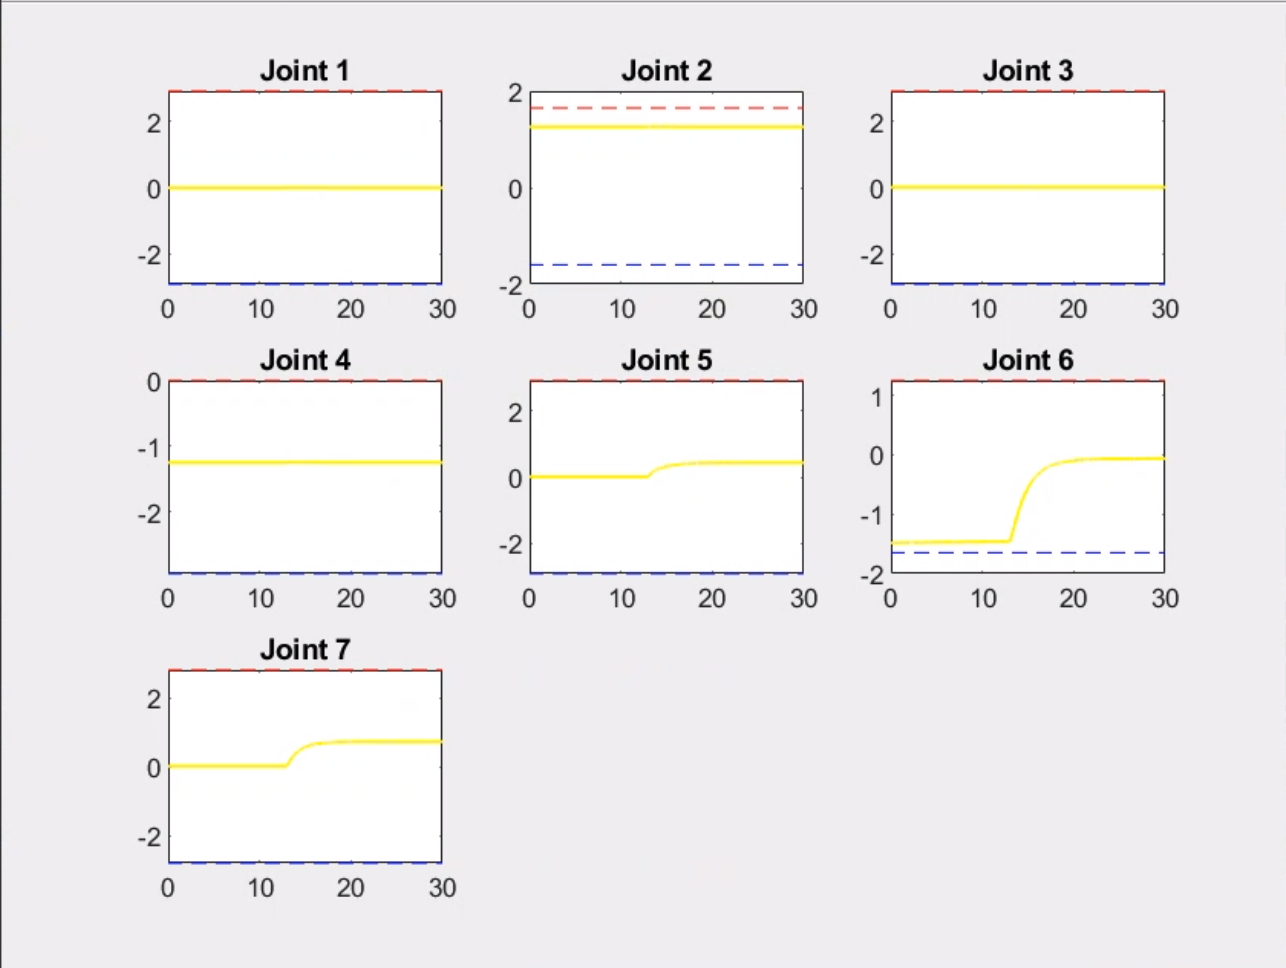
\includegraphics[width=\textwidth]{522_1_wout_TPIK2.png} 
\caption[Joint limits: without TPIK2]{Joint limits: without TPIK2}\label{JL_wout_TPIK2} 
\end{minipage} 
\hspace{0.2\textwidth} 
\begin{minipage}{0.40\textwidth}  
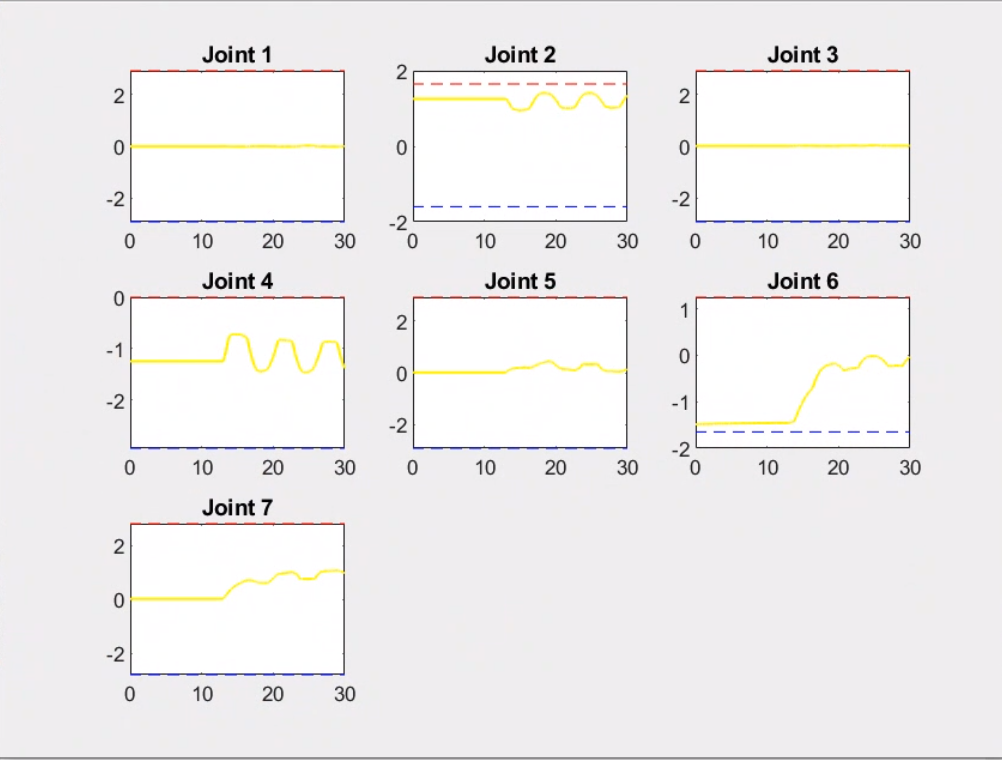
\includegraphics[width=\textwidth]{522_1_w_TPIK2.png}
\caption[Joint limits: with TPIK2]{Joint limits: with TPIK2}\label{JL_w_TPIK2} 
\end{minipage}  
\end{figure}
%%%%%%%% MINI PAGE IMAGES %%%%%%%%
\begin{figure}[htpb] 
\begin{minipage}{0.40\textwidth} 
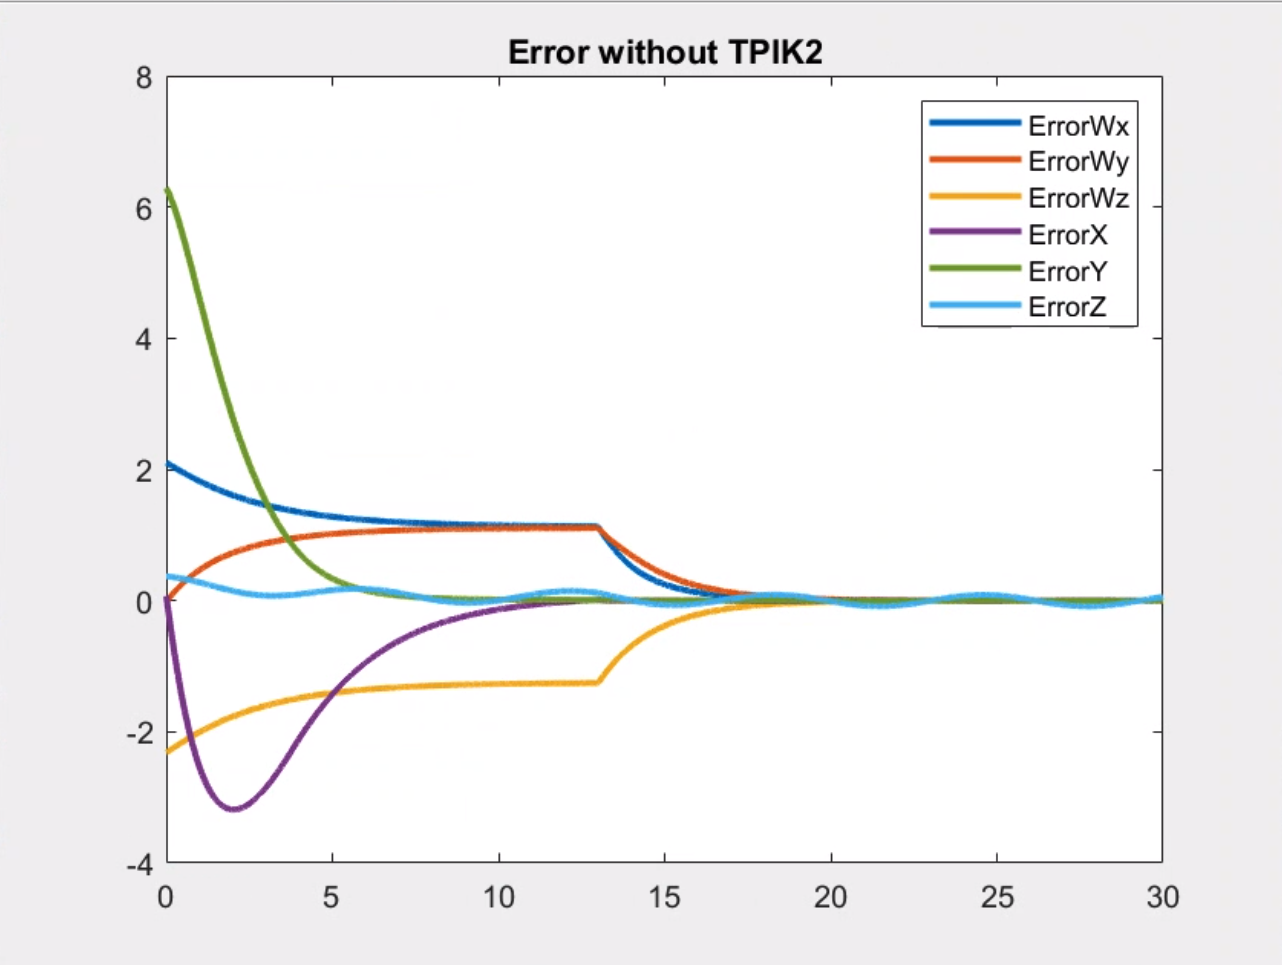
\includegraphics[width=\textwidth]{522_2_wout_TPIK2.png} 
\caption[Errors: without TPIK2]{Errors: without TPIK2}\label{Error_wout_TPIK2} 
\end{minipage} 
\hspace{0.2\textwidth} 
\begin{minipage}{0.40\textwidth}  
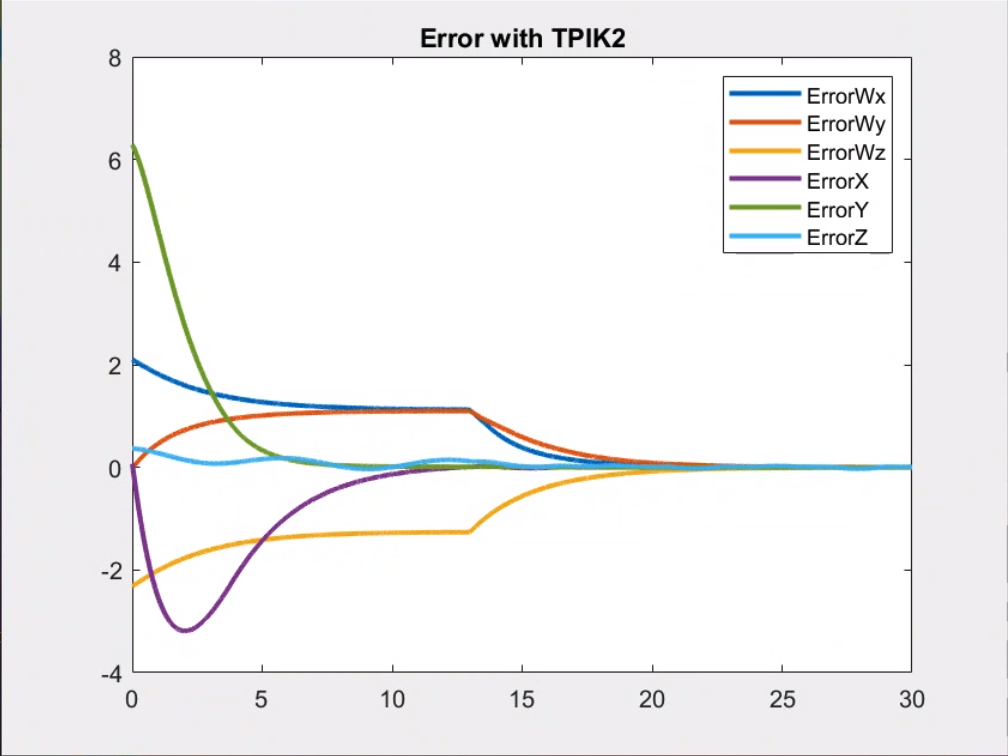
\includegraphics[width=\textwidth]{522_2_w_TPIK2.png}
\caption[Errors: with TPIK2]{Errors: with TPIK2}\label{Error_w_TPIK2} 
\end{minipage}  
\end{figure}
%%%%%%%% MINI PAGE IMAGES %%%%%%%%
\begin{figure}[htpb] 
\begin{minipage}{0.40\textwidth} 
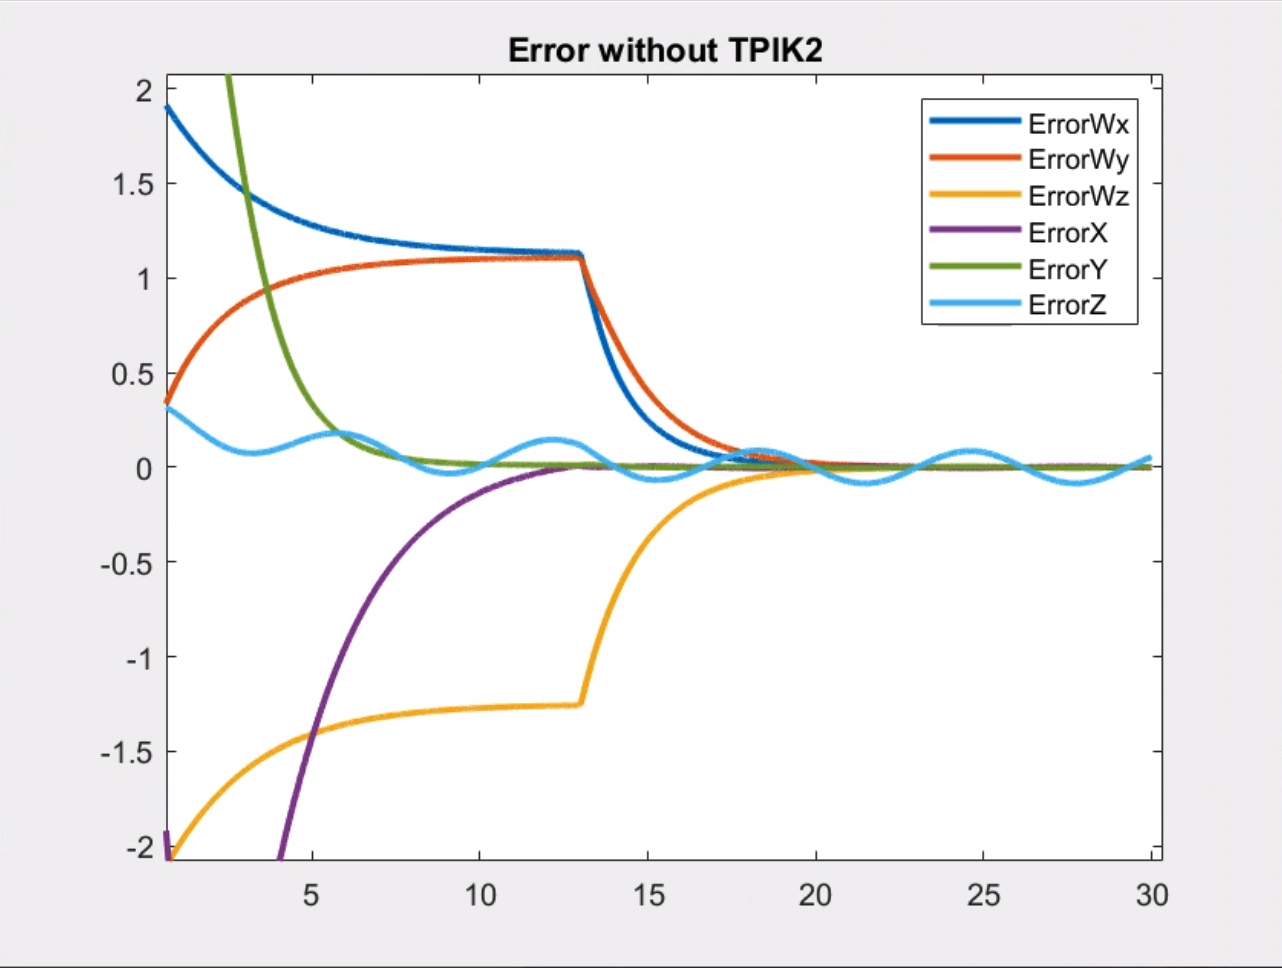
\includegraphics[width=\textwidth]{522_3_wout_TPIK2.png} 
\caption[Zoomed Error: without TPIK2]{Zoomed Error: without TPIK2}\label{zoomed_error_wout_TPIK2} 
\end{minipage} 
\hspace{0.2\textwidth} 
\begin{minipage}{0.40\textwidth}  
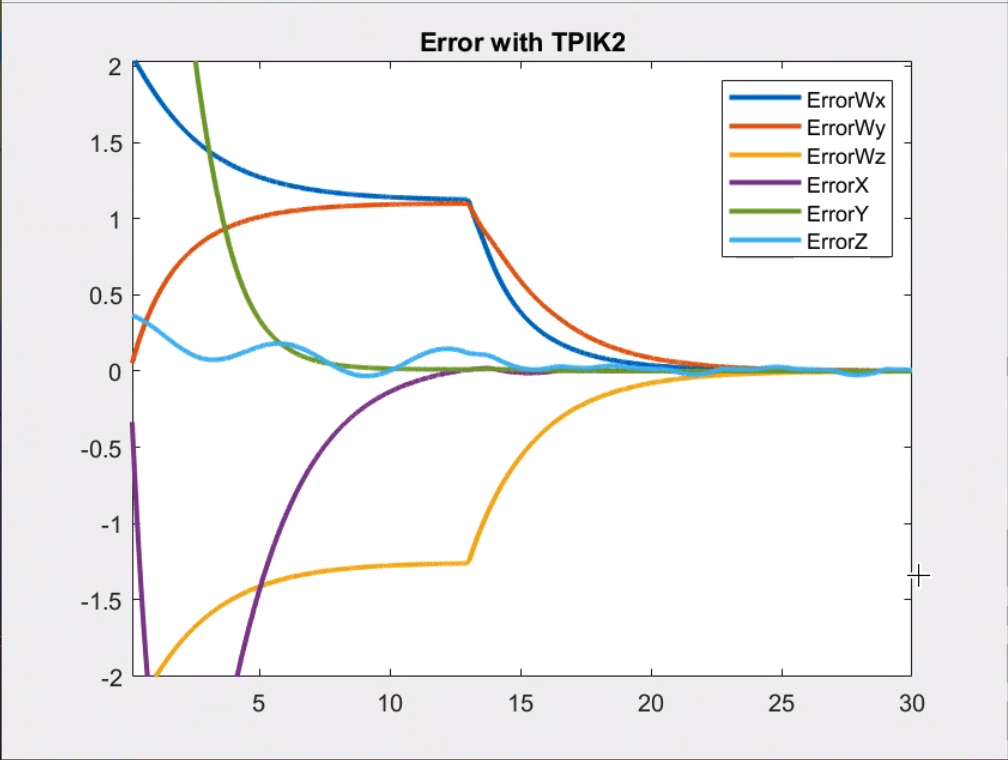
\includegraphics[width=\textwidth]{522_3_w_TPIK2.png}
\caption[Zoomed Error: with TPIK2]{Zoomed Error: with TPIK2}\label{zoomed_error_w_TPIK2} 
\end{minipage}  
\end{figure}
%%%%%%%% MINI PAGE IMAGES %%%%%%%%
\begin{figure}[htpb] 
\begin{minipage}{0.40\textwidth} 
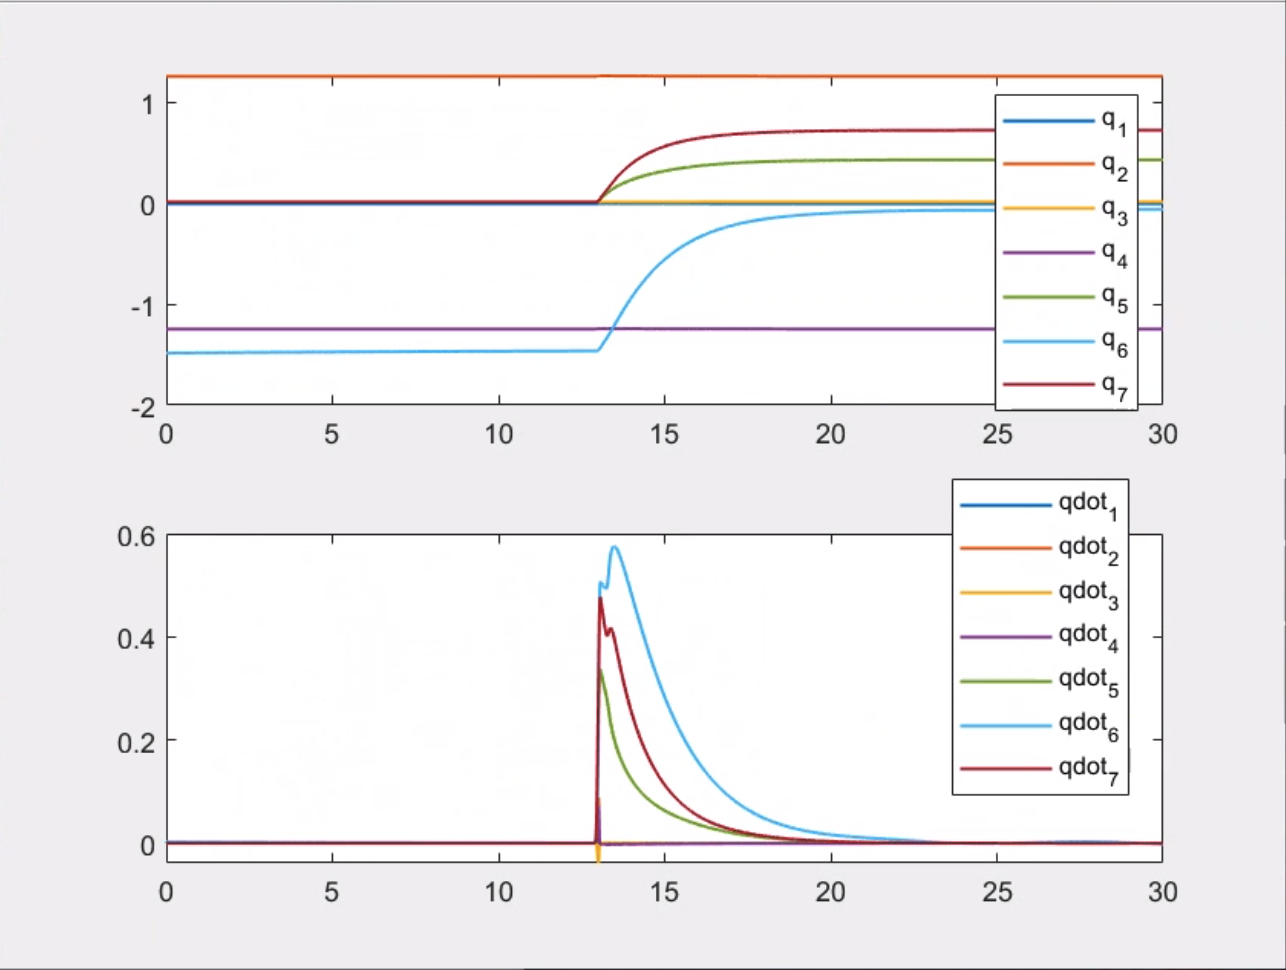
\includegraphics[width=\textwidth]{522_4_wout_TPIK2.png} 
\caption[Joints configurations and velocities: without TPIK2]{Joints configurations and velocities: without TPIK2}\label{Jqandqdot_wout_TPIK2} 
\end{minipage} 
\hspace{0.2\textwidth} 
\begin{minipage}{0.40\textwidth}  
\includegraphics[width=\textwidth]{522_4_w_TPIK2.png}
\caption[Joints configurations and velocities: with TPIK2]{Joints configurations and velocities: with TPIK2}\label{Jqandqdot_w_TPIK2} 
\end{minipage}  
\end{figure}

\end{document}

